\chapter{整除, 同余和不定方程}
\section{整除}
任意两个整数的和, 差或积都是整数, 但是两个整数做除法时所得的结果不一定是整数, 因此, 数论中的许多问题都是在研究整数之间的除法.

\subsection{整除的概念与基本性质}
\begin{definition}
对任给的两个整数 $a ,  b(a \neq 0)$, 如果存在整数 $q$, 使得 $b=a q$,那么称 $b$ 能被 $a$ 整除(或称 $a$ 能整除 $b$ ), 记作 $a \mid b$. 否则, 称 $b$ 不能被 $a$ 整除, 记作 $a \nmid b$ . 

如果 $a \mid b$, 那么称 $a$ 为 $b$ 的因数, $b$ 为 $a$ 的倍数.
\end{definition}

利用整除的定义,可以非常容易地推导出下面一些经常被用到的性质. 

\begin{property}
如果 $a \mid b$, 那么 $a \mid(-b)$ ,反过来也成立; 进一步,如果 $a \mid b$, 那么 $(-a) \mid b$ ,反过来也成立.
\end{property}

因此,我们经常只讨论正整数之间的整除关系.

\begin{property}
如果 $a|b, b| c$, 那么 $a \mid c$ . 这表明整除具有传递性.
\end{property}

\begin{property}
若 $a|b, a| c$, 则对任意整数 $x ,  y$, 都有 $a \mid b x+c y$ . (即 $a$ 能整除 $b ,  c$ 的任意一个“线性组合”)
\end{property}

% 例 1
\begin{example}
若 $a|n, b| n$, 且存在整数 $x ,  y$, 使得 $a x+b y=1$, 证明: $a b \mid n$.
\end{example}
\begin{proof}
由条件, 可设 $n=a u, n=b v, u ,  v$ 为整数. 于是\\
\begin{align*}
n & =n(a x+b y) \\
& =n a x+n b y \\
& =a b v x+a b u y \\
& =a b(v x+u y)
\end{align*}

因此
\begin{equation*}
a b \mid n
\end{equation*}
\end{proof}
\begin{note}
一般地, 由 $a|n, b| n$, 并不能推出 $a b \mid n$, 例如 $2|6,6| 6$, 但 $12 \nmid 6$. 题中给出的条件实质上表明 $a ,  b$ 的最大公因数 (见 1.3 节) 为 1 , 即 $a$与 $b$ 互素,在此条件下可推出 $a b \mid n$ . 
\end{note}

% 例 2
\begin{example}
证明:无论在数 12008 的两个 0 之间添加多少个 3 ,所得的数都是 19 的倍数. 
\end{example}
\begin{proof}
记 $a_{0}=12008, a_{n}=120 \underbrace{3 \cdots 308}_{n \uparrow 3}, n=1,2, \cdots$.

首先,因为
\begin{align*}
a_{0}=19 \times 632
\end{align*}

故
\begin{align*}
19 \mid a_{0}
\end{align*}

其次,设 $19 \mid a_{n}$ ,则由
\begin{align*}
a_{n+1}-10 a_{n}=228=19 \times 12
\end{align*}

可知
\begin{align*}
19 \mid a_{n+1} \cdot
\end{align*}

所以,对一切整数 $n$ ,数 $a_{n}$ 都是 19 的倍数.
\end{proof}
\begin{note}
此题的处理过程中运用了递推的思想,其基本思路是将 $a_{n+1}$ 表示为 $a_{n}$ 与 19 的一个线性组合. 
\end{note}

% 例 3
\begin{example}
已知一个 1000 位正整数的任意连续 10 个数码形成的 10 位数是 $2^{10}$ 的倍数. 证明:该正整数为 $2^{1000}$ 的倍数. 
\end{example}
\begin{proof}
设该正整数 $x=\overline{a_{1} a_{2} \cdots a_{1000}}$, 其中 $a_{i}$ 是十进位数码. 由条件, 可知
\begin{align}
2^{10} \mid & \overline{a_{991} \cdots a_{1000}}, 2^{10} \mid \overline{a_{990} \cdots a_{999}},
\end{align}
因此
\begin{align}\label{eq:2024_10_09_1}
2^{10} \mid \overline{a_{990} \cdots a_{999}} & \times 10.
\end{align}

记 $y=\overline{a_{991} \cdots a_{999}}$ ,则\autoref{eq:2024_10_09_1}又可写作
\begin{align*}
2^{10} \mid a_{990} \times 10^{10}+10 y,
\end{align*}

故
\begin{align*}
2^{10} \mid 10 y.
\end{align*}

结合 $2^{10} \mid \overline{a_{991} \cdots a_{1000}}$ ,可知
\begin{align*}
2^{10} \mid 10 y+a_{1000},
\end{align*}

于是
\begin{align*}
2^{10} \mid a_{1000},
\end{align*}

这要求
\begin{align*}
a_{1000}=0.
\end{align*}

类似地,朝前倒推,可得
\begin{align*}
a_{11}=\cdots=a_{1000}=0,
\end{align*}

即
\begin{align*}
x=\overline{a_{1} \cdots a_{10}} \times 10^{990}.
\end{align*}

再结合条件 $2^{10} \mid \overline{a_{1} \cdots a_{10}}$ ,即可得
\begin{align*}
2^{1000} \mid x.
\end{align*}
\end{proof}
\begin{note}
这里先证明 $a_{11}=\cdots=a_{1000}=0$ 是非常关键的,在证明中利用 $\overline{a_{991} \cdots a_{999}}$ 来过渡也是比较巧妙的. 
\end{note}

例 4 设 $m$ 是一个大于 2 的正整数,证明:对任意正整数 $n$ ,都有 $2^{m}-1 \nmid$ $2^{n}+1$.

证明 如果存在正整数 $n$, 使得 $2^{m}-1 \mid 2^{n}+1$ ,那么取其中最小的那个 $n$ . 

由于 $m>2$, 知 $n>1$, 进一步, 应有 $2^{n}+1 \geqslant 2^{m}-1$, 知 $n \geqslant m$ ,而 $n=m$时,将导致 $2^{m}-1 \mid 2$ (因为 $2=\left(2^{n}+1\right)-\left(2^{n}-1\right)$ ,右边每一项都是 $2^{n}-1$ 的倍数),矛盾,故 $n>m$ . 

现在,设 $2^{n}+1=\left(2^{m}-1\right) q$ ,这里 $q$ 为正整数,则
\begin{align*}
2^{n}+2^{m}=\left(2^{n}+1\right)+\left(2^{m}-1\right)=\left(2^{m}-1\right)(q+1)
\end{align*}

即
\begin{align*}
2^{m}\left(2^{n \sqcap m}+1\right)=\left(2^{m}-1\right)(q+1)
\end{align*}

于是,
\begin{align*}
\left(2^{n-m}+1\right)+\left(2^{m}-1\right)\left(2^{n-m}+1\right)=\left(2^{m}-1\right)(q+1)
\end{align*}

得 $2^{n-m}+1=\left(2^{m}-1\right)\left(q-2^{n-m}\right)$ ,因此, $2^{m}-1 \mid 2^{n-m}+1$ ,与 $n$ 的最小性矛盾. 

所以,命题成立.

说明 这里用到了两个结论:一个是 "若 $a \mid b, b \neq 0$ ,则 $|a| \leqslant|b| "$ ,它由整除的定义可直接证出. 另一个是"任意多个正整数中必有最小元",这是著名的"最小数原理". 

\subsection{素数与合数}
对任意正整数 $n>1$, 如果除 1 与 $n$ 以外, $n$ 没有其他的因数,那么称 $n$ 为素数. 否则称 $n$ 为合数. 这样,我们将正整数分为了三类: 1 ,素数,合数. 

素数从小到大依次为 $2,3,5,7,11, \cdots$ . 我们可以非常轻松地写出 100以内的所有素数,共 25 个. 但是并不是对每个素数 $p$ ,都能轻易地指出 $p$ 后面的一个素数是多少. 事实上,当 $p$ 比较大时,求出它后面的那个素数是十分困难的. 正是素数的这种无规律性,初等数论才显得魅力无穷, 具有很强的挑战

性和极大的吸引力. \\
素数与合数具有如下的一些性质. \\
性质1 设 $n$ 为大于 1 的正整数, $p$ 是 $n$ 的大于 1 的因数中最小的正整数, 则 $p$ 为素数.

性质2 如果对任意 1 到 $\sqrt{n}$ 之间的素数 $p$, 都有 $p \nmid n$, 那么 $n$ 为素数. 这里 $n(>1)$ 为正整数.

证明 事实上, 若 $n$ 为合数, 则可写 $n=p q, 2 \leqslant p \leqslant q$. 因此 $p^{2} \leqslant n$, 即 $p \leqslant \sqrt{n}$ . 

这表明 $p$ 的素因子 $\leqslant \sqrt{n}$ ,且它是 $n$ 的因数,与条件矛盾. 因此 $n$ 为素数.\\
说明 这里素因子是指正整数的因数中为素数的那些数, 此性质是我们检验一个数是否为素数的最常用的方法. 

性质3 素数有无穷多个.\\
证明 若只有有限个素数, 设它们是 $p_{1}<p_{2}<\cdots<p_{n}$. 考虑数\\
\begin{align*}
x=p_{1} p_{2} \cdots p_{n}+1
\end{align*}

其最小的大于 1 的因数 $p$, 它是一个素数, 因此, $p$ 应为 $p_{1}, p_{2}, \cdots, p_{n}$ 中的某个数. 设 $p=p_{i}, 1 \leqslant i \leqslant n$, 并且 $x=p_{i} y$, 则 $p_{1} p_{2} \cdots p_{n}+1=p_{i} y$, 即 $p_{i}(y-$ $\left.p_{1} p_{2} \cdots p_{i-1} p_{i+1} \cdots p_{n}\right)=1$. 这导致 $p_{i} \mid 1$. 矛盾.

所以, 素数有无穷多个.\\
说明 如果将所有的素数从小到大依次写出为 $2=p_{1}<p_{2}<\cdots$, 并写 $q_{n}=p_{1} p_{2} \cdots p_{n}+1$, 那么\\
\begin{align*}
q_{1}=3, q_{2}=7, q_{3}=31, q_{4}=211, q_{5}=2311
\end{align*}

它们都是素数. 是否每一个 $n$ 都有 $q_{n}$ 为素数呢? 我们不能被表面现象所迷惑, 再朝下算, 可知 $q_{6}=59 \times 509$ 就是一个合数. 事实上, 后面的 $q_{7}, q_{8}, q_{9}$, $q_{10}$ 都是合数. 到目前为止, 人们还不知道数列 $q_{1}, q_{2}, \cdots$ 中是否有无穷多个素数, 也不知道其中是否有无穷多个合数.

性质4 素数中只有一个数是偶数,它是 2 . \\
例1 设 $n$ 为大于 1 的正整数. 证明: 数 $n^{5}+n^{4}+1$ 不是素数.\\
证明 注意到\\
\begin{align}
& n^{5}+n^{4}+1 \\
= & n^{5}+n^{4}+n^{3}-\left(n^{3}-1\right) \\
= & n^{3}\left(n^{2}+n+1\right)-(n-1)\left(n^{2}+n+1\right) \\
= & \left(n^{3}-n+1\right)\left(n^{2}+n+1\right)
\end{align}

因此, 若 $n^{5}+n^{4}+1$ 为素数, 则 $n^{3}-n+1=1$, 这要求 $n=0$ 或 $\pm 1$ . \\
故当 $n>1$ 时, $n^{5}+n^{4}+1$ 不是素数. \\
说明 利用因式分解来判断一个数是否为素数是数论中的常见方法,后面也将不断用到. 

例 2 考察下面的数列:\\
\begin{align*}
101,10101,1010101, \cdots
\end{align*}

问:该数列中有多少个素数?\\
解 易知 101 是素数. 下证这是该数列中仅有的一个素数. \\
\begin{align}
& \text { 记 } a_{n}=\underbrace{10101 \cdots 01}_{n \text { 个 } 01} \text {, 则当 } n \geqslant 2 \text { 时,有 } \\
& a_{n}=10^{2 n}+10^{2(n-1)}+\cdots+1 \\
& =\frac{10^{2(n+1)}-1}{10^{2}-1} \\
& =\frac{\left(10^{n+1}-1\right)\left(10^{n+1}+1\right)}{99} .
\end{align}

注意到, $99<10^{n+1}-1,99<10^{n+1}+1$ ,而 $a_{n}$ 为正整数,故 $a_{n}$ 是一个合数(因为分子中的项 $10^{n+1}-1$ 与 $10^{n+1}+1$ 都不能被 99 约为 1 ). 

说明 这里需要将因式分解式 $x^{n}-1=(x-1)\left(x^{n-1}+x^{n-2}+\cdots+1\right)$ 反用,高中阶段它被作为等比数列求和的公式. 

例 3 求所有的正整数 $n$, 使得 $\frac{n(n+1)}{2}-1$ 是一个素数.\\
解 记 $a_{n}=\frac{n(n+1)}{2}-1$ ,则 $a_{1}=0$ 不是素数,因此只需讨论 $n>1$ 的情形. 我们利用 $n$ 只能是形如 $4 k ,  4 k+1 ,  4 k+2 ,  4 k+3$ 的数分别讨论.

当 $n$ 是形如 $4 k+2$ 或 $4 k+1$ 的数时, $a_{n}$ 都是偶数, 要 $a_{n}$ 为素数, 只能是\\
\begin{align*}
\begin{gathered}
\frac{n(n+1)}{2}-1=2 \\
n=2
\end{gathered}
\end{align*}

解得\\
当 $n=4 k$ 时,可得\\
\begin{align}
a_{n} & =2 k(4 k+1)-1 \\
& =8 k^{2}+2 k-1 \\
& =(4 k-1)(2 k+1),
\end{align}

这是一个合数.\\
当 $n=4 k+3$ 时, 可得\\
\begin{align}
a_{n} & =2(k+1)(4 k+3)-1 \\
& =8 k^{2}+14 k+5 \\
& =(4 k+5)(2 k+1),
\end{align}

仅当 $k=0$ ,即 $n=3$ 时, $a_{n}$ 为素数. \\
所以,满足条件的 $n=2$ 或 3.\\
说明 对 $n$ 分类处理一方面是去分母的需要,另一方面是为进行因式分解做准备. 

例 4 对任意正整数 $n$ ,证明:存在连续 $n$ 个正整数,它们都是合数. \\
证明 设 $n$ 为正整数,则\\
\begin{align*}
(n+1)!+2,(n+1)!+3, \cdots,(n+1)!+(n+1)
\end{align*}

是 $n$ 个连续正整数, 并且第 $k$ 个数是 $k+1$ 的倍数(且大于 $k+1$ ),故它们是连续的 $n$ 个合数. 

说明 这个结论表明:对任意正整数 $n$ ,都存在两个素数,它们之间至少有 $n$ 个数,且这些数都是合数. 但是,让我们来看一些素数对(3,5),(5,7),\\
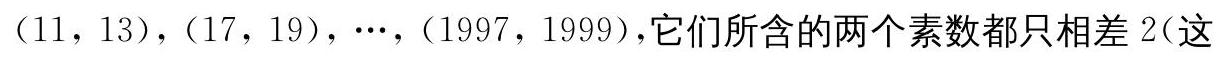
\includegraphics[width=.5\textwidth]{2024_10_09_7e48ff928cc374c97394g-016}是两个奇素数的最小差距),这样的素数对称为孪生素数. 是否存在无穷多对素数,它们是孪生素数?这是数论中一个未解决的著名问题. 

例5 设 $n$ 为大于 2 的正整数. 证明:存在一个素数 $p$ ,满足 $n<p<n!$ . \\
证明 设 $p_{1}<p_{2}<\cdots<p_{k} ,$ 且 $p_{1}, p_{2}, \cdots, p_{k}$ 是所有不超过 $n$ 的素数,考虑数\\
\begin{align*}
q=p_{1} p_{2} \cdots p_{k}-1
\end{align*}

在 $n>2$ 时, 2,3 都在 $p_{1}, \cdots, p_{k}$ 中出现,故 $5 \leqslant q \leqslant n!-1<n!$ ,利用性质 3 证明中的方法,可知 $q$ 的素因子 $p$ 不等于 $p_{1}, p_{2}, \cdots, p_{k}$ 中的任何一个. 而 $p_{1}, p_{2}, \cdots, p_{k}$ 是所有不超过 $n$ 的素数,因此 $p>n$ ,所以 $n<p \leqslant q<n$ !.

从而,命题成立. \\
说明 利用本题的结论亦可证出:素数有无穷多个. 贝特朗曾猜测在 $m>1$ 时,正整数 $m$ 与 $2 m$ 之间(不包括 $m$ 与 $2 m$ )有一个素数. 如果将素数从小到大排列为 $p_{1}<p_{2}<\cdots$ ,该猜测亦即 $p_{n+1}<2 p_{n}$ . 这个猜测被契比雪夫证明了. 因此它被称为贝特朗猜想或契比雪夫定理. 

例6 设 $a ,  b ,  c ,  d ,  e ,  f$ 都是正整数, $S=a+b+c+d+e+f$ 是 $a b c+$ $d e f$ 和 $a b+b c+c a-d e-e f-e d$ 的因数. 证明: $S$ 为合数. 

证明 考虑多项式\\
\begin{align*}
f(x)=(x+a)(x+b)(x+c)-(x-d)(x-e)(x-f)
\end{align*}

展开后, 可知\\
\begin{align*}
f(x)=S x^{2}+(a b+b c+c a-d e-e f-f d) x+(a b c+d e f)
\end{align*}

由条件可知,对任意 $x \in \mathbf{Z}$ ,都有 $S \mid f(x)$ . 特别地,取 $x=d$ ,就有 $S \mid f(d)$ ,即 $S \mid(d+a)(d+b)(d+c)$ . 由于 $a ,  b ,  c ,  d ,  e ,  f$ 都为正整数,故 $d+a ,  d+b$ ,  $d+c$ 都小于 $S$, 所以, $S$ 为合数. 

说明 对比例2,两个例子中分别用到下面的结论:若 $x ,  y ,  z$ 为正整数,且 $\frac{x y}{z}$ 亦为整数,则如果 $x ,  y>z$, 那么 $\frac{x y}{z}$ 为合数;如果 $x ,  y<z$, 那么 $z$ 为合数.

\subsection{最大公因数与最小公倍数}
设 $a ,  b$ 是不全为零的两个整数, $d$ 是一个非零整数,如果 $d \mid a$ 且 $d \mid b$ ,那么称 $d$ 为 $a ,  b$ 的公因数. 

注意到,当 $d \mid a$ 且 $d \mid b$ 时,则 $d \leqslant|a|$ 或 $d \leqslant|b|$ 中必有一个成立(对 $a ,  b$ 中不为零的数成立). 因此, $a ,  b$ 的公因数中有一个最大的, 这个数称为 $a ,  b$ 的最大公因数,记为 $(a, b)$ . 如果 $(a, b)=1$ ,那么我们称 $a ,  b$ 互素. 

在讨论最大公因数的性质之前,我们不加证明地引入一个在小学就接触到的, 数论中最基本, 最常用的结论. 

带余数除法 设 $a ,  b$ 是两个整数, $a \neq 0$, 则存在唯一的一对整数 $q$ 和 $r$,满足\\
\begin{align*}
b=a q+r, 0 \leqslant r<|b|
\end{align*}

其中 $q$ 称为 $b$ 除以 $a$ 所得的商, $r$ 称为 $b$ 除以 $a$ 所得的余数.\\
性质1 设 $d=(a, b)$ ,则存在整数 $x ,  y$ ,使得\\
\begin{align*}
a x+b y=d
\end{align*}

这个结论就是著名的贝祖(Bezout)定理. \\
证明 我们利用带余除法来处理,此结论的证明过程又是求 $a ,  b$ 的最大公因数的过程,它被称为"辗转相除". 

不妨设 $a ,  b$ 都不为零(当 $a ,  b$ 中有一个为零时,结论是显然的),且 $|a| \leqslant|b|$.

设 $b=a q_{1}+r_{1}$, 其中 $0 \leqslant r_{1}<|a|, q_{1} ,  r_{1}$ 为整数. 若 $r_{1}=0$ ,则辗转相

除到此为止; 否则用 $a$ 去除以 $r_{1}$, 得等式 $a=r_{1} q_{2}+r_{2}, 0 \leqslant r_{2}<r_{1}$; 依此讨论, 由于 $r_{1}>r_{2}>r_{3}>\cdots$, 因此辗转相除到某一步后, 所得的 $r_{k+1}=0$, 于是,我们得到了如下的一系列式子:\\
\begin{align}
b & =a q_{1}+r_{1}, 0<r_{1}<|a| \\
a & =r_{1} q_{2}+r_{2}, 0<r_{2}<r_{1} \\
r_{1} & =r_{2} q_{3}+r_{3}, 0<r_{3}<r_{2} \\
\cdots & \cdots \cdots \cdots \cdots \cdots \cdots \cdots \cdots \cdots \\
r_{k-2} & =r_{k-1} q_{k}+r_{k}, 0<r_{k}<r_{k-1} \\
r_{k-1} & =r_{k} q_{k+1}
\end{align}

注意到, 从第一个式子到第 $k$ 个式子,我们依次有\\
\begin{align*}
d\left|r_{1}, d\right| r_{2}, \cdots, d \mid r_{k},
\end{align*}

而从第 $k+1$ 个式子倒推, 又依次有\\
\begin{align*}
r_{k}\left|r_{k-1}, r_{k}\right| r_{k-2}, \cdots, r_{k}\left|r_{1}, r_{k}\right| a, r_{k} \mid b,
\end{align*}

所以, $r_{k}$ 又是 $a ,  b$ 的公因数, 结合 $d$ 为 $a ,  b$ 的最大公因数知 $r_{k} \leqslant d$, 又 $d \mid r_{k}$,故 $d \leqslant r_{k}$, 因此, $d=r_{k}$ . 也就是说, 我们求出了 $a ,  b$ 的最大公因数.

现在, 利用 $d=r_{k}$ 及第 $k$ 个式子, 可知\\
\begin{align*}
d=r_{k-2}-r_{k-1} q_{k}
\end{align*}

再由\\
\begin{align*}
r_{k-1}=r_{k-3}-r_{k-2} q_{k-1}(\text { 第 } k-1 \text { 个式子变形得 }),
\end{align*}

代入上式, 可知 $d$ 可以表示为 $r_{k-2}$ 与 $r_{k-3}$ 的"线性组合" (见 1.1 节性质2), 依此倒推, 可知 $d$ 可以表示为 $a, b$ 的"线性组合", 即存在整数 $x, y$ 使得\\
\begin{align*}
d=a x+b y .
\end{align*}

说明反过来, 设 $x ,  y$ 为整数, $d^{\prime}=a x+b y$, 并不能推出 $d^{\prime}$ 为 $a ,  b$ 的最大公因数. 事实上, 可以证明: $a ,  b$ 的最大公因数是形如 $a x+b y$ ( $x, y$ 为任意整数) 的正整数中最小的那个.

性质2 设 $d$ 为 $a ,  b$ 的公因数, 则 $d \mid(a, b)$ . \\
这个性质可由前面的贝祖定理证出. 事实上, 贝祖定理也是初等数论中的一个基本定理,应用非常广泛,下面的性质是它的一个直接推论.

性质3 设 $a ,  b$ 是不全为零的整数, 则 $a$ 与 $b$ 互素的充要条件是存在整数 $x ,  y$ 满足\\
\begin{align*}
a x+b y=1
\end{align*}

性质4 设 $a|c, b| c$ ,且 $(a, b)=1$ ,则 $a b \mid c$ . \\
这个性质的证明见 1.1 节的例 1.\\
性质5 设 $a \mid b c$ ,且 $(a, b)=1$ ,则 $a \mid c$ . \\
证明 由性质3,知存在整数 $x, y$ 使得\\
\begin{align*}
a x+b y=1
\end{align*}

故 $a c x+b c y=c$ ,由 $a \mid b c$ 及 $a \mid a c x$ ,可知 $a \mid c$ . \\
性质6 设 $p$ 为素数, $p \mid a b$ ,则 $p \mid a$ 或 $p \mid b$ . \\
证明 由于 $p$ 只有两个正约数,故 $(p, a)=1$ 或者 $(p, a)=p$ . 若 $(p, a)=$ 1 ,则由性质 5 知 $p \mid b$ ;若 $(p, a)=p$ ,则 $p \mid a$ . 

下面引入公倍数的一些概念和性质. \\
设 $a ,  b$ 都是不等于零的整数,如果整数 $c$ 满足 $a \mid c$ 且 $b \mid c$ ,那么称 $c$ 为 $a ,  b$ 的公倍数. 在 $a ,  b$ 的所有正的公倍数中,最小的那个称为 $a ,  b$ 的最小公倍数,记作 $[a, b]$ . 

性质7 设 $a ,  b$ 为非零整数, $d ,  c$ 分别是 $a ,  b$ 的一个公因数与公倍数,则 $d|(a, b),[a, b]| c$ . 

证明 这个性质在本质上反映了最大公因数与最小公倍数的属性. 前者是性质2的结论,这里再次列出是为了对比. 

对于后者,采用反证法予以证明. \\
若 $[a, b] \nmid c$ ,设 $c=[a, b] \cdot q+r, 0<r<[a, b]$ ,则由 $a \mid c$ 及 $a \mid[a, b]$ ,可知 $a \mid r$ ,同理 $b \mid r$ ,即 $r$ 为 $a ,  b$ 的公倍数,但 $r<[a, b]$ ,这与 $[a, b]$ 是 $a ,  b$ 的最小公倍数矛盾. 所以 $[a, b] \mid c$ . 

性质8 设 $a ,  b$ 都是正整数,则 $[a, b]=\frac{a b}{(a, b)}$.\\
证明 记 $c=\frac{a b}{(a, b)}$, 则由 $(a, b) \mid a$ 及 $(a, b) \mid b$ 知 $b|c, a| c$ . 即 $c$ 为 $a ,  b$ 的公倍数,故 $[a, b] \mid c$ . 

反过来,由贝祖定理,知存在整数 $x ,  y$ ,使得

即\\
\begin{align*}
a x+b y=(a, b)
\end{align*}\\
\begin{align*}
\frac{a}{(a, b)} x+\frac{b}{(a, b)} y=1
\end{align*}

于是\\
\begin{align*}
\frac{a[a, b]}{(a, b)} x+\frac{b[a, b]}{(a, b)} y=[a, b]
\end{align*}

由 $b \mid[a, b]$ 及 $a \mid[a, b]$, 可知\\
\begin{align*}
c\left|\frac{a[a, b]}{(a, b)}, c\right| \frac{b[a, b]}{(a, b)}
\end{align*}

所以\\
\begin{align*}
c \mid[a, b]
\end{align*}

综上, 可知\\
\begin{align*}
[a, b]=\frac{a b}{(a, b)}
\end{align*}

一般地,对 $n$ 个整数(非零) $a_{1}, a_{2}, \cdots, a_{n}$ ,可以类似地引入最大公因数与最小公倍数的概念,分别记为 $\left(a_{1}, a_{2}, \cdots, a_{n}\right)$ 和 $\left[a_{1}, a_{2}, \cdots, a_{n}\right]$ . 容易得到下面的一些结论:

性质9 $\left(a_{1}, a_{2}, a_{3}, \cdots, a_{n}\right)=\left(\left(a_{1}, a_{2}\right), a_{3}, \cdots, a_{n}\right)$ ;而 $\left[a_{1}, a_{2}\right.$, $\left.a_{3}, \cdots, a_{n}\right]=\left[\left[a_{1}, a_{2}\right], a_{3}, \cdots, a_{n}\right]$.

性质10 存在整数 $x_{1}, x_{2}, \cdots, x_{n}$ ,使得\\
\begin{align*}
a_{1} x_{1}+a_{2} x_{2}+\cdots+a_{n} x_{n}=\left(a_{1}, a_{2}, \cdots, a_{n}\right)
\end{align*}

特别地, $\left(a_{1}, a_{2}, \cdots, a_{n}\right)=1$ ,即 $a_{1}, a_{2}, \cdots, a_{n}$ 互素的充要条件是:存在整数 $x_{1}, x_{2}, \cdots, x_{n}$, 使得\\
\begin{align*}
a_{1} x_{1}+a_{2} x_{2}+\cdots+a_{n} x_{n}=1
\end{align*}

注意, $n$ 个数互素,并不能保证它们两两互素,例如( $2 \times 3,2 \times 5,3 \times$ $5 )=1$ ,但 6,  $10 ,  15$ 两两不互素. 反过来,若 $n$ 个数中有两个数互素,则这 $n$个数互素. 因此,在 $n$ 个数中,"两两互素"的条件比"它们互素"的条件要强得多. 

性质11 设 $m$ 为正整数, 则\\
\begin{align}
& \left(m a_{1}, m a_{2}, \cdots, m a_{n}\right)=m\left(a_{1}, a_{2}, \cdots, a_{n}\right) \\
& {\left[m a_{1}, m a_{2}, \cdots, m a_{n}\right]=m\left[a_{1}, a_{2}, \cdots, a_{n}\right]}
\end{align}

例1 设 $a ,  b$ 为正整数,且 $\frac{a b}{a+b}$ 也是正整数. 证明: $(a, b)>1$ . \\
证明 若 $(a, b)=1$ ,则 $(a, a+b)=1$ (这由性质 3 可推得),从而,由 $a+b \mid a b$ 及 $(a, a+b)=1$ ,得 $a+b \mid b$ ,但是 $a+b>b$ ,故 $a+b \mid b$ 不可能成立. 所以, $(a, b)>1$.

说明 在辗转相除求 $a ,  b$ 的公因数的讨论中,可知对任意整数 $x$ ,都有 $(a, b)=(a, b+a x)$, 这一点在利用最大公因数处理数论问题时经常被用到. 

例 2 设正整数 $a ,  b ,  c$ 满足 $b^{2}=a c$ . 证明: $(a, b)^{2}=a(a, c)$.\\
证明 如果我们能够证明: $(a, b)^{2}=\left(a^{2}, b^{2}\right)$ ,那么结合性质11,可知\\
\begin{align*}
(a, b)^{2}=\left(a^{2}, b^{2}\right)=\left(a^{2}, a c\right)=a(a, c)
\end{align*}

命题获证.\\
为此,记 $d=(a, b)$ ,设 $a=d u, b=d v$ ,则由性质11可知 $u ,  v$ 是两个互素的正整数,为证 $\left(a^{2}, b^{2}\right)=d^{2}$ ,只需证明: $\left(u^{2}, v^{2}\right)=1$ . 

利用贝祖定理,知存在整数 $x ,  y$ ,使得 $u x+v y=1$ ,故 $u^{2} x^{2}=(1-v y)^{2}=$ $1+v\left(v y^{2}-2 y\right)$ ,结合性质 3 可知 $\left(u^{2}, v\right)=1$ ,交换 $u^{2}$ 与 $v$ 的位置,同上再做一次,即有 $\left(v^{2}, u^{2}\right)=1$ . 

所以,命题成立. \\
说明 利用下一节的算术基本定理可以非常方便地证出: $\left(a^{2}, b^{2}\right)=$ $(a, b)^{2}$ ,但遗憾的是我们还没给出该定理的证明,通常都是先建立最大公因数理论再去证算术基本定理,这里不用该定理是不希望掉入"循环论证"的旋涡,读者在学习中应认真掌握其中的逻辑结构. 

例 3 求所有的正整数 $a ,  b(a \leqslant b)$ ,使得\\
\begin{align*}
a b=300+7[a, b]+5(a, b)
\end{align*}

解 设 $[a, b]=x,(a, b)=y$ ,由性质 8 可知 $a b=x y$ ,于是,(1)变为\\
\begin{align*}
x y=300+7 x+5 y
\end{align*}

即 $(x-5)(y-7)=5 \times 67$ . \\
由于 $[a, b] \geqslant(a, b)$, 故 $x \geqslant y$, 进而 $x-5>y-7$, 只有如下的两种情形. 

情形一 $x-5=67$ 且 $y-7=5$ ;此时, $x=72, y=12$ ,于是,可设 $a=12 n , b=12 m ,(m, n)=1$ ,并有 $(12 n)(12 m)=a b=x y=12 \times 72$ ,结合 $a \leqslant b$ ,只能是 $(m, n)=(1,6)$ 或 $(2,3)$ ,对应的 $(a, b)=(12,72)$ 或 $(24$ , 36).

情形二 $\quad x-5=335$ 且 $y-7=1$ ;对应地, $x=340, y=8$ ,但 $y=(a ,$ $b )$ 是 $x=[a, b]$ 的因数, 而 8 ł 340 ,所以,此时无解. 

综上,符合条件的 $(a, b)=(12,72)$ 或 $(24,36)$ . \\
例 4 求所有的正整数 $a ,  b$, 使得\\
\begin{align*}
(a, b)+9[a, b]+9(a+b)=7 a b
\end{align*}

解 记 $(a, b)=d$ ,设 $a=d x, b=d y$ ,则 $(x, y)=1$ (由性质11知), $[a, b]=d x y$ (由性质 8 知),于是代入(1)可得\\
\begin{align*}
1+9 x y+9(x+y)=7 d x y
\end{align*}\\
\begin{align*}
7 d=9+9\left(\frac{1}{x}+\frac{1}{y}\right)+\frac{1}{x y}
\end{align*}

所以\\
\begin{align*}
9<7 d \leqslant 9+9\left(\frac{1}{1}+\frac{1}{1}\right)+\frac{1}{1 \times 1}=28
\end{align*}

故\\
\begin{align*}
2 \leqslant d \leqslant 4
\end{align*}

当 $d=2$ 时, 由(2)得\\
\begin{align*}
5 x y-9(x+y)=1
\end{align*}

两边乘以 5 ,并将左边因式分解,得\\
\begin{align*}
(5 x-9)(5 y-9)=86=2 \times 43
\end{align*}

故 $(5 x-9,5 y-9)=(1,86) , (86,1),(2,43) , (43,2)$. 分别求解可知只能是 $(x, y)=(2,19),(19,2)$ ,对应的 $(a, b)=(4,38),(38,4)$ . 

分别就 $d=3,4$ 同上讨论,得 $(a, b)=(4,4)$ . \\
所以,满足条件的 $(a, b)=(4,38),(38,4),(4,4)$ . \\
例 5 Fibonacci 数列定义如下: $F_{1}=F_{2}=1, F_{n+2}=F_{n+1}+F_{n}, n=1$ , $2, \cdots$ . 证明:对任意正整数 $m ,  n$ ,都有 $\left(F_{m}, F_{n}\right)=F_{(m, n)}$ . 

证明 当 $m=n$ 时,命题显然成立. 现在不妨设 $m<n$ ,注意到\\
\begin{align}
F_{n} & =F_{2} F_{n-1}+F_{1} F_{n-2} \\
& =F_{2}\left(F_{n-2}+F_{n-3}\right)+F_{1} F_{n-2} \\
& =\left(F_{2}+F_{1}\right) F_{n-2}+F_{2} F_{n-3} \\
& =F_{3} F_{n-2}+F_{2} F_{n-3} \\
& =F_{3}\left(F_{n-3}+F_{n-4}\right)+F_{2} F_{n-3} \\
& =F_{4} F_{n-3}+F_{3} F_{n-4} \\
& =\cdots \\
& =F_{m} F_{n-m+1}+F_{m-1} F_{n-m},
\end{align}

因此, 设 $d \mid F_{m}$ 且 $d \mid F_{n}$, 则由上式可知 $d \mid F_{m-1} F_{n \rightarrow m}$. 又对任意正整数 $m$ ,有 $\left(F_{m}, F_{m-1}\right)=\left(F_{m-1}+F_{m-2}, F_{m-1}\right)=\left(F_{m-1}, F_{m-2}\right)=\cdots=\left(F_{2}, F_{1}\right)=1$,所以, $\left(d, F_{m-1}\right)=1$, 故 $d \mid F_{n-m}$; 反过来, 若 $d^{\prime} \mid F_{n-m}$ 且 $d^{\prime} \mid F_{m}$, 则由上式又可知 $d^{\prime} \mid F_{n}$ . 依此可知 $\left(F_{n}, F_{m}\right)=\left(F_{n-m}, F_{m}\right)$ . 

利用上述结论, 对下标进行辗转相除, 就可证得 $\left(F_{n}, F_{m}\right)=F_{(m, n)}$.\\
说明 由本题的结论还可以推出一个有趣的性质: 若 $F_{n}$ 为素数, 则 $n=4$或者 $n$ 为素数. 

事实上, 设 $F_{n}$ 为素数, 而 $n$ 为合数, 可设 $n=p \cdot q, 2 \leqslant p \leqslant q, p ,  q$ 为正

整数, 则由前面的结论, 可知 $\left(F_{n}, F_{p}\right)=F_{(n, p)}=F_{p},\left(F_{n}, F_{q}\right)=F_{(n, q)}=$ $F_{q}$ . 结合 Fibonacci 数列的定义,可知 $F_{n}>F_{p}, F_{n}>F_{q}$ ,而 $F_{n}$ 为素数,故 $\left(F_{n}, F_{p}\right)=\left(F_{n}, F_{q}\right)=1$ ,所以, $F_{p}=F_{q}=1$ ,再由 $2 \leqslant p \leqslant q$ ,可知只能是 $p=q=2$ ,即 $n=4$ . 所以,性质成立. 

例 6 设 $n$ 为大于 1 的正整数. 证明:存在从小到大排列后成等差数列 (即从第二项起, 每一项与它前面那项的差为常数的数列) 的 $n$ 个正整数,它们中任意两项互素. 

证明 考虑下面的 $n$ 个数:\\
\begin{align*}
n!+1,2 \times(n!)+1, \cdots, n \times(n!)+1
\end{align*}

这 $n$ 个正整数组成一个公差为 $n!$ 的等差数列.\\
我们证明其中任意两项是互素的. \\
事实上,若存在 $1 \leqslant i<j \leqslant n$ ,使得数 $i \times(n!)+1$ 与数 $j \times(n!)+1$ 不互素,设 $d=(i \times(n!)+1, j \times(n!)+1)>1$ . 考虑 $d$ 的素因子 $p$ ,可知\\
\begin{align*}
p \mid(j \times(n!)+1)-(i \times(n!)+1)
\end{align*}

即 $p \mid(j-i) \times n$ !. 由性质 6 知 $p \mid j-i$ 或 $p \mid n!$ ,结合 $1 \leqslant j-i<n$ ,可知 $(j-i) \mid n!$ ,所以,总有 $p \mid n!$ . 但是, $p|d, d| i \times(n!)+1$ ,故 $p \mid i \times(n!)+1$ ,结合 $p \mid n!$ ,导致 $p \mid 1$ ,矛盾. 

所以,命题成立. \\
说明 此题为导出与反设矛盾的结论,采用了素因子分析的方法. 该方法在数论中有广泛的应用. 

\subsection{算术基本定理}
在 1.2 节中我们引入了素数与合数的概念,对每个大于 1 的正整数 $n$ ,如果 $n$ 为合数,那么可写 $n=n_{1} n_{2}$ ,其中 $2 \leqslant n_{1} \leqslant n_{2}$ . 再分别对 $n_{1} ,  n_{2}$ 重复这样的讨论,即可将 $n$ 表示为一些素数的乘积. 对这个过程认真思考,就能得到下面的重要定理,在解数论的问题时经常会直接或间接地用到它. 

算术基本定理 设 $n$ 是大于 1 的正整数,则 $n$ 可以分解成若干个素数的乘积的形式,并且在不考虑这些素数相乘时的前后次序时,这种分解是唯一的. 即对任意大于 1 的正整数 $n$,都存在唯一的一种素因数分解形式:\\
\begin{align*}
n=p_{1}^{\alpha_{1}} p_{2}^{\alpha_{2}} \cdots p_{k}^{\alpha_{k}}
\end{align*}

这里 $p_{1}<p_{2}<\cdots<p_{k}$ 为素数, $\alpha_{1}, \alpha_{2}, \cdots, \alpha_{k}$ 为正整数. 

证明 利用前面的分析,可证得存在性,下面证明唯一性. \\
若 $n$ 有两种素因数分解形式:\\
\begin{align*}
n=p_{1}^{\alpha_{1}} p_{2}^{\alpha_{2}} \cdots p_{k}^{\alpha_{k}}=q_{1}^{\beta_{1}} q_{2}^{\beta_{2}} \cdots q_{l}^{\beta_{2}}
\end{align*}

其中 $p_{1}<p_{2}<\cdots<p_{k}, q_{1}<q_{2}<\cdots<q_{l}$ ,且都是素数, $\alpha_{i} ,  \beta_{j}$ 都为正整数, $1 \leqslant i \leqslant k, 1 \leqslant j \leqslant l$.

我们证明 $k=l$ 且 $p_{i}=q_{i}, \alpha_{i}=\beta_{i}$ . \\
事实上,由(1)知 $p_{i} \mid q_{1}^{\beta_{1}} q_{2}^{\beta_{2}} \cdots q_{l}^{\beta_{l}}$ ,利用前一节的性质6可知,存在某个 $j$ 使 $p_{i} \mid q_{j}^{\beta_{j}}$ ,再用一次性质6,知 $p_{i} \mid q_{j}$ ,这要求 $p_{i}=q_{j}$ . 即对 $1 \leqslant i \leqslant k$ 及每个 $p_{i}$ ,在 $q_{1}, q_{2}, \cdots, q_{l}$ 中总有一个 $q_{j}$ ,使得 $p_{i}=q_{j}$ . 反过来对 $q_{j}$ 分析,又有对 $1 \leqslant$ $j \leqslant l$ 及每个 $q_{j}$ ,在 $p_{1}, p_{2}, \cdots, p_{k}$ 中总有一个 $p_{i}$ ,使得 $q_{j}=p_{i}$ . 这表明 $k=l$ ,且 $q_{1}, q_{2}, \cdots, q_{l}$ 是 $p_{1}, p_{2}, \cdots, p_{k}$ 的一个排列,结合 $p_{1}<p_{2}<\cdots<p_{k}$ 及 $q_{1}<q_{2}<\cdots<q_{l}$ ,知 $p_{i}=q_{i}, 1 \leqslant i \leqslant k$ . 进一步证明 $\alpha_{i}=\beta_{i}$ 是容易的. 

利用正整数 $n$ 的素因数分解式,我们可以简单地得到下面的一些结论. \\
$1^{\circ}$ 设 $n$ 的所有正因数(包括 1 和 $n$ )的个数为 $d(n)$ ,那么\\
\begin{align*}
d(n)=\left(\alpha_{1}+1\right)\left(\alpha_{2}+1\right) \cdots\left(\alpha_{k}+1\right)
\end{align*}

由此公式易知: $n$ 是一个完全平方数的充要条件是 $d(n)$ 为奇数. \\
$2^{\circ}$ 设 $n$ 的所有正因数之和为 $\sigma(n)$ ,那么\\
\begin{align*}
\sigma(n)=\left(1+p_{1}+\cdots+p_{1}^{\alpha_{1}}\right)\left(1+p_{2}+\cdots+p_{2}^{\alpha_{2}}\right) \cdots\left(1+p_{k}+\cdots+p_{k}^{\alpha_{k}}\right)
\end{align*}

由此可知: $\sigma(n)$ 为奇数的充要条件是 $n$ 为完全平方数或者某个完全平方数的两倍. \\
$3^{\circ}$ 设 $n ,  m$ 的素因数分解分别为\\
\begin{align*}
n=p_{1}^{\alpha_{1}} p_{2}^{\alpha_{2}} \cdots p_{k}^{\alpha_{k}}, m=p_{1}^{\beta_{1}} p_{2}^{\beta_{2}} \cdots p_{k}^{\beta_{k}},
\end{align*}

这里 $p_{1}<p_{2}<\cdots<p_{k}$ ,都为素数, $\alpha_{i} ,  \beta_{i}$ 都是非负整数,并且对每个 $1 \leqslant i \leqslant$ $k, \alpha_{i}$ 与 $\beta_{i}$ 不全为零,那么,我们有 $(m, n)=p_{1}^{\gamma_{1}} p_{2}^{\gamma_{2}} \cdots p_{k}^{\gamma_{k}}$ ; $[m, n]=$ $p_{1}^{\delta_{1}} p_{2}^{\delta_{2}} \cdots p_{k}^{\delta_{k}}$ ,其中 $\gamma_{i}=\min \left\{\alpha_{i}, \beta_{i}\right\}, \delta_{i}=\max \left\{\alpha_{i}, \beta_{i}\right\}, 1 \leqslant i \leqslant k$ . 

例1 在一个走廊上依次排列着编号为 $1,2, \cdots, 2012$ 的灯共 2012 盏,最初每盏灯的状态都是开着的. 一个好动的学生做了下面的 2012 次操作:对 $1 \leqslant k \leqslant 2012$ ,该学生第 $k$ 次操作时,将所有编号是 $k$ 的倍数的灯的开关都拉了一下. 问:最后还有多少盏灯是开着的?

解 设 $1 \leqslant n \leqslant 2012$ ,我们来考察第 $n$ 盏灯的状态,依题意,该盏灯的开关被拉了 $d(n)$ 次. 而偶数次拉动开关不改变灯的初始状态,奇数次拉动开关,

灯的状态与初始状态不同.\\
利用 $d(n)$ 的性质及前面的讨论, 因为 $1,2, \cdots, 2012$ 中恰有 44 个数为完全平方数, 可知最后还有 $2012-44=1968$ 盛灯是开着的.

例 2 求所有的正整数 $n$, 使得 $n=d(n)^{2}$ . \\
解 当 $n=1$ 时, 符合条件, 下面考虑 $n>1$ 的情形.\\
由条件知 $n$ 为完全平方数, 因此 $d(n)$ 为奇数, 设 $d(n)=2 k+1$. 鉴于对任意正整数 $d$, 当 $d \mid n$ 时, 有 $\left.\frac{n}{d} \right\rvert\, n$, 因此, 我们将 $d$ 与 $\frac{n}{d}$ 配对后, 可知 $d(n)$ 等于数 $1,2, \cdots, 2 k-1$ 中为 $n$ 的因数的个数的两倍加上 1 . 又 $1,2, \cdots, 2 k-1$中的偶数都不是 $n\left(=(2 k+1)^{2}\right)$ 的因数, 因此结合 $d(n)=2 k+1$, 可知 1 , $2, \cdots, 2 k-1$ 中的每一个奇数都是 $n$ 的因数.

注意到, 当 $k>1$ 时, $(2 k-1,2 k+1)=(2 k-1,2)=1$, 故 $2 k-1 \nmid$ $(2 k+1)^{2}$. 所以 $k>1$ 时, $n=(2 k+1)^{2}$ 不符合要求,故 $k=1, n$ 只能等于 9 .

直接验证, 可知 1 和 9 满足条件, 所以 $n=1$ 或 9.\\
说明 此题考虑了 $n$ 的因数关于 $\sqrt{n}$ 的对称性, 分析出一个非常强的条件, 从而解决了问题.

它还有一个一般性的处理方法, 需要用到如下的估计: 设 $p$ 为不小于 5的素数, 则 $p^{\alpha}>(\alpha+1)^{2}$. 而 $\alpha \geqslant 2$ 时, $3^{\alpha} \geqslant(\alpha+1)^{2}$. 这两个不等式都可以用数学归纳法予以证明(对 $\alpha$ 归纳). 

现在设 $n(>1)$ 是一个满足条件的正整数, 则 $n$ 为一个奇数的平方, 于是, 可设 $n=3^{\alpha} \cdot p_{1}^{\beta_{1}} p_{2}^{\beta_{2}} \cdots p_{k}^{\beta_{k}}$, 其中 $3<p_{1}<p_{2}<\cdots<p_{k}$, 并且 $\alpha, \beta_{1}$, $\beta_{2}, \cdots, \beta_{k}$ 都是偶数. 如果 $k>0$, 那么由前面的分析, 知 $n>(\alpha+1)^{2}\left(\beta_{1}+1\right)^{2} \cdot$ $\left(\beta_{2}+1\right)^{2} \cdots\left(\beta_{k}+1\right)^{2}=d(n)^{2}$, 矛盾, 故 $n=3^{\alpha}$. 进一步分析, 可知 $\alpha>2$ 时, 有 $3^{\alpha}>(\alpha+1)^{2} ,$ 故 $\alpha=2$, 即 $n=9$.

例3 设 $n$ 为正整数. 证明:数 $2^{2^{n}}+2^{2^{n-1}}+1$ 至少有 $n$ 个不同的素因子.证明 我们作如下的分解:\\
\begin{align}
& 2^{2^{n}}+2^{2^{n-1}}+1 \\
= & \left(2^{2^{n-1}}+1\right)^{2}-2^{2^{n-1}} \\
= & \left(2^{2^{n-1}}+2^{2^{n-2}}+1\right)\left(2^{2^{n-1}}-2^{2^{n-2}}+1\right) \\
= & \left(2^{2^{n-2}}+2^{2^{n-3}}+1\right)\left(2^{2^{n-2}}-2^{2^{n-3}}+1\right)\left(2^{2^{n-1}}-2^{2^{n-2}}+1\right) \\
= & \cdots \\
= & \left(2^{2^{1}}+2^{2^{0}}+1\right)\left(2^{2^{1}}-2^{2^{0}}+1\right)\left(2^{2^{2}}-2^{2^{1}}+1\right) \cdots\left(2^{2^{n-1}}-2^{2^{n-2}}+1\right)
\end{align}

这样, 我们将 $2^{2^{n}}+2^{2^{n-1}}+1$ 表示为 $n$ 个大于 1 的正整数之积, 为证明它有 $n$ 个不同的素因子,只需证明这 $n$ 个大于 1 的正整数两两互素. 

注意到, 当 $m>l$ 时, $2^{2^{l}}+2^{2^{L-1}}+1$ 与 $2^{2^{l}}-2^{2^{L-1}}+1$ 都是 $2^{2^{m}}+2^{2^{m-1}}+1$的因数, 因此\\
\begin{align}
& \left(2^{2^{m}}-2^{2^{m-1}}+1,2^{2^{l}} \pm 2^{2^{L-1}}+1\right) \\
\leqslant & \left(2^{2^{m}}-2^{2^{m-1}}+1,2^{2^{m}}+2^{2^{m-1}}+1\right) \\
= & \left(2^{2^{m}}-2^{2^{m-1}}+1,2 \times 2^{2 m-1}\right)
\end{align}

由于, $2 \times 2^{2 m-1}$ 中只有一个素因子 2 , 而 $2^{2^{m}}-2^{2^{m-1}}+1$ 为奇数, 故

因此\\
\begin{align*}
\left(2^{2^{m}}-2^{2^{m-1}}+1,2 \times 2^{2^{m-1}}\right)=1,
\end{align*}\\
\begin{align*}
\left(2^{2^{m}}-2^{2 m-1}+1,2^{2^{l}} \pm 2^{2^{2-1}}+1\right)=1 .
\end{align*}

所以, $2^{2^{1}}+2^{2^{0}}+1,2^{2^{1}}-2^{2^{0}}+1,2^{2^{2}}-2^{2^{1}}+1, \cdots, 2^{2^{n-1}}-2^{2^{n-2}}+1$ 两两互素,进而 $2^{2^{n}}+2^{2^{n-1}}+1$ 至少有 $n$ 个不同的素因子. 

例 4 设 $m ,  n$ 是正整数, 且 $m$ 的所有正因数之积等于 $n$ 的所有正因数之积. 问: $m$ 与 $n$ 是否必须相等?

解 $m$ 与 $n$ 必须相等.\\
事实上, 将 $m$ 的正因数 $d$ 与 $\frac{m}{d}$ 配对, 可知 $m$ 的所有正因数之积为 $m \frac{d(m)}{2}$,因此, 条件等价于\\
\begin{align*}
m^{d(n)}=n^{d(n)},
\end{align*}

此式表明 $m ,  n$ 有相同的素因子, 可设\\
\begin{align*}
m=p_{1}^{a_{1}} p_{2}^{a_{2}} \cdots p_{k}^{\alpha_{k}}, n=p_{1}^{\beta_{1}} p_{2}^{\beta_{2}} \cdots p_{k}^{\beta_{k}},
\end{align*}

其中 $p_{1}<p_{2}<\cdots<p_{k}$ 为素数 $\alpha_{i}$ 与 $\beta_{i}$ 都是正整数, $1 \leqslant i \leqslant k$.\\
代入(1)式,利用算术基本定理, 可知\\
\begin{align*}
\alpha_{i} d(m)=\beta_{i} d(n), 1 \leqslant i \leqslant k,
\end{align*}

若 $d(m)>d(n)$, 则对 $1 \leqslant i \leqslant k$, 都有 $\alpha_{i}<\beta_{i}$, 于是, $\alpha_{i}+1<\beta_{i}+1$, 故 $\left(\alpha_{1}+1\right)\left(\alpha_{2}+1\right) \cdots\left(\alpha_{k}+1\right)<\left(\beta_{1}+1\right)\left(\beta_{2}+1\right) \cdots\left(\beta_{k}+1\right)$, 这导致 $d(m)<$ $d(n)$ ,矛盾. 同样,由 $d(m)<d(n)$ ,利用(2)式也可导出矛盾. 所以 $d(m)=$ $d(n)$ ,进而由(1)式得 $m=n$.

说明 一般地, 由 $\sigma(m)=\sigma(n)$ (即考虑 $m ,  n$ 所有正因数之和) 并不能导出 $m=n$ (例如 $\sigma(6)=\sigma(11)=12$ ), 此题是对两个正整数的所有正因数作乘积方面的思考得出的结论.

例 5 求所有的正整数 $x, y$, 使得\\
\begin{align*}
y^{x}=x^{50}
\end{align*}

解 设 $x ,  y$ 为满足条件的正整数,并且 $x=p_{1}^{\alpha_{1}} p_{2}^{\alpha_{2}} \cdots p_{k}^{\alpha_{k}}$ 为 $x$ 的素因数分解式,则

由 $y$ 为正整数,知对 $1 \leqslant i \leqslant k$ ,都有 $x \mid 50 \alpha_{i}$ . 现在先讨论 $x$ 的素因子. \\
如果 $x$ 有一个不同于 2 和 5 的素因子 $p$ ,并设 $p^{\alpha} \| x$ ,那么由前面的结果知 $x \mid 50 \alpha$ ,当然有 $p^{\alpha} \mid 50 \alpha$ ,又 $p \neq 2 ,  5$ ,故 $p^{\alpha} \mid \alpha$ . 但是,对任意素数 $p$ 及正整数 $\alpha$ ,有 $p^{\alpha}>\alpha$ ,所以, $p^{\alpha} \mid \alpha$ 不能成立,这表明 $x$ 的素因子只能为 2 或 5 . 

于是,我们可设 $x=2^{\alpha} \cdot 5^{\beta}$ (其中 $\alpha ,  \beta$ 为非负整数),这时 $x|50 \alpha, x| 50 \beta$ ,故 $2^{\alpha}\left|50 \alpha, 5^{\beta}\right| 50 \beta$ ,前者要求 $2^{\alpha-1} \mid \alpha$ ,后者要求 $5^{\beta-2} \mid \beta$ . 注意到,当 $\alpha \geqslant 3$ 时, $2^{\alpha-1}>\alpha$, 而 $\beta \geqslant 3$ 时, $5^{\beta-2}>\beta$ ,所以, $0 \leqslant \alpha \leqslant 2,0 \leqslant \beta \leqslant 2$ . 这表明 $x$ 只能取 $1,2,2^{2}, 5,5^{2}, 2 \times 5,2^{2} \times 5,2 \times 5^{2}, 2^{2} \times 5^{2}$ . 

将 $x$ 的上述取值逐个代入 (1)式,可得到全部解为 $(x, y)=(1,1)$ , $\left(2,2^{25}\right),\left(2^{2}, 2^{25}\right),\left(5,5^{10}\right),\left(5^{2}, 5^{4}\right),\left(10,10^{5}\right),(50,50),(100,10)$,共 8 组解.

说明 上面两例直接用到算术基本定理,所涉及的变量数看似增加或会变难,但这时不等式估计的手段可介入,问题求解反而有了着力点. 

例 6 给定正整数 $n>1$ ,设 $d_{1}, d_{2}, \cdots, d_{n}$ 都是正整数,满足: $\left(d_{1}, d_{2}, \cdots\right.$ , $\left.d_{n}\right)=1$ ,且对 $j=1,2, \cdots, n$ 都有 $d_{j} \mid \sum_{i=1}^{n} d_{i}\left(\right.$ 这里 $\sum_{i=1}^{n} d_{i}=d_{1}+d_{2}+\cdots+$ $\left.d_{n}\right)$.\\
(1)证明: $d_{1} d_{2} \cdots d_{n} \mid\left(\sum_{i=1}^{n} d_{i}\right)^{n-2}$ ;\\
(2)举例说明: $n>2$ 时,上式右边的幂次不能减小.\\
证明 (1)设 $p$ 为 $d_{1} d_{2} \cdots d_{n}$ 的素因数,且 $k$ 为各 $d_{i}$ 的素因数分解式中 $p$的幂次的最大值, 则由 $d_{j} \mid \sum_{i=1}^{n} d_{i}$ 可知, $p^{k} \mid \sum_{i=1}^{n} d_{i}$, 故 $p^{k(n-2)} \mid\left(\sum_{i=1}^{n} d_{i}\right)^{n-2}$.

而 $\left(d_{1}, d_{2}, \cdots, d_{n}\right)=1$ ,故存在 $d_{i}$ ,使得 $p \nmid d_{i}$ ,结合 $p \mid \sum_{i=1}^{n} d_{i}$ ,可知 $d_{1}$ , $d_{2}, \cdots, d_{n}$ 中至少有两个数不是 $p$ 的倍数. 所以, $p$ 在 $d_{1} d_{2} \cdots d_{n}$ 中的幂次不超过 $k(n-2)$ ,依此可知结论成立. \\
(2)设 $d_{1}=1, d_{2}=n-1, d_{i}=n, 3 \leqslant i \leqslant n$ ,则 $\sum_{i=1}^{n} d_{i}=n(n-1)$ 是每个 $d_{i}$ 的倍数,且 $\left(d_{i}, d_{2}, \cdots, d_{n}\right)=1$.

此时, $d_{1} d_{2} \cdots d_{n}=n^{n-2}(n-1)$ ,结合 $(n, n-1)=1$ ,可知满足 $n^{n-2}(n-$ 1) $\mid(n(n-1))^{m}$ 的最小正整数 $m=n-2$.

\subsection{习题 1}
1 设 $n$ 为大于 1 的正整数. 证明: $n^{4}+4^{n}$ 是一个合数. \\
2 求使得 $\left|4 x^{2}-12 x-27\right|$ 为素数的所有整数 $x$ . \\
3 设 $m$ 为大于 1 的正整数,且 $m \mid(m-1)!+1$ . 证明: $m$ 是一个素数. \\
4 是否存在 3 个不同的素数 $p ,  q ,  r$ ,使得下面的整除关系都成立?\\
\begin{align*}
q r\left|p^{2}+d, r p\right| q^{2}+d, p q \mid r^{2}+d
\end{align*}

其中(1) $d=10 ; ( 2 ) d=11$ . \\
5 设 $p$ 为正整数,且 $2^{p}-1$ 是素数. 求证: $p$ 为素数. \\
6 设 $n$ 为正整数,且 $2^{n}+1$ 是素数. 证明:存在非负整数 $k$ ,使得 $n=2^{k}$ . \\
7 求所有形如 $n^{n}+1$ 且不超过 $10^{19}$ 的素数,这里 $n$ 为正整数. \\
8 设 $a ,  b ,  c ,  d$ 都是整数,且 $a \neq c, a-c \mid a b+c d$ . 证明: $a-c \mid a d+b c$ . \\
9 设 $a ,  b ,  c ,  d$ 为整数,且 $a c ,  b c+a d ,  b d$ 都是某个整数 $u$ 的倍数. 证明:数 $b c$ 和 $a d$ 也是 $u$ 的倍数. \\
10 设 $a ,  b ,  n$ 为给定的正整数,且对任意正整数 $k(\neq b)$ ,都有 $b-k \mid a-k^{n}$ . 证明: $a=b^{n}$ . \\
11 已知正整数 $n$ 的正因数中,末尾数字为 $0,1,2, \cdots, 9$ 的正整数都至少有一个. 求满足条件的最小的 $n$ . \\
12 求一个 9 位数 $M$ ,使得 $M$ 的数码两两不同且都不为零,并对 $m=2,3, \cdots$ , 9 ,数 $M$ 的左边 $m$ 位数都是 $m$ 的倍数. \\
13 对于一个正整数 $n$ ,若存在正整数 $a ,  b$ ,使得 $n=a b+a+b$ ,则称 $n$ 是一个"好数",例如 $3=1 \times 1+1+1$ ,故 3 为一个"好数". 问:在 $1,2, \cdots, 100$中,有多少个"好数"?\\
14 设素数从小到大依次为 $p_{1}, p_{2}, p_{3}, \cdots$ . 证明:当 $n \geqslant 2$ 时,数 $p_{n}+p_{n+1}$ 可以表示为 3 个大于 1 的正整数(可以相同)的乘积的形式. \\
15 设 $n$ 为大于 1 的正整数. 证明: $n$ 为合数的充要条件是存在正整数 $a ,  b$ ,  $x ,  y$ ,使得 $n=a+b, \frac{x}{a}+\frac{y}{b}=1$ . \\
16 证明:数列 $10001,100010001,1000100010001, \cdots$ 中,每一个数都是合数.

17 设 $a ,  b ,  c ,  d$ 都是素数,且 $a>3 b>6 c>12 d, a^{2}-b^{2}+c^{2}-d^{2}=1749$.求 $a^{2}+b^{2}+c^{2}+d^{2}$ 的所有可能值. \\
18 数列 $\left\{a_{n}\right\}$ 的每一项都是正整数, $a_{1} \leqslant a_{2} \leqslant a_{3} \leqslant \cdots$ ,且对任意正整数 $k$ ,该数列中恰有 $k$ 项等于 $k$ . 求所有的正整数 $n$ ,使得 $a_{1}+a_{2}+\cdots+a_{n}$ 是素数. \\
19 由正整数组成的数列 $\left\{a_{n}\right\}$ 满足:对任意正整数 $m$ ,  $n$ ,若 $m \mid n , m<n$ ,则 $a_{m} \mid a_{n}$ ,且 $a_{m}<a_{n}$ . 求 $a_{2000}$ 的最小可能值. \\
20 设 $p$ 为奇素数,正整数 $m ,  n$ 满足 $\frac{m}{n}=1+\frac{1}{2}+\cdots+\frac{1}{p-1}$ . 证明: $p \mid m$ . \\
21 设 $a ,  m ,  n$ 为正整数, $a>1$ ,且 $a^{m}+1 \mid a^{n}+1$ . 证明: $m \mid n$ . \\
22 证明:对任意正整数 $n$ 及正奇数 $m$ ,都有 $\left(2^{m}-1,2^{n}+1\right)=1$ . \\
23 费马数 $F_{n}$ 定义为 $F_{n}=2^{2^{n}}+1$. 证明:对任意两个不同的正整数 $m ,  n$ ,都有 $\left(F_{n}, F_{m}\right)=1$\\
24 已知正整数 $a ,  b ,  c ,  d$ 的最小公倍数为 $a+b+c+d$. 证明: $a b c d$ 是 3 或 5 的倍数. \\
25 记 $M_{n}$ 为正整数 $1,2, \cdots, n$ 的最小公倍数. 求所有的正整数 $n(>1)$, 使得 $M_{n}=M_{n-1}$ . \\
26 设 $a ,  m ,  n$ 为正整数, $a>1$ . 证明: $\left(a^{m}-1, a^{n}-1\right)=a^{(m, n)}-1$ . \\
27 设 $a ,  n$ 为正整数, $a>1$ ,且 $a^{n}+1$ 是素数. 证明: $d\left(a^{n}-1\right) \geqslant n$ . \\
28 对怎样的正整数 $n(>2)$ ,存在 $n$ 个连续正整数,使得其中最大的数是其余 $n-1$ 个数的最小公倍数的因数?\\
29 设正整数 $a ,  b ,  m ,  n$ 满足: $(a, b)=1, a>1$ ,且 $a^{m}+b^{m} \mid a^{n}+b^{n}$ . 证明: $m \mid n$\\
30 证明:存在 2012 个不同的正整数,使得其中任意两个不同的数 $a ,  b$ 都满足 $(a-b)^{2} \mid a b$.\\
31 设 $a ,  b$ 为正整数,且 $(a, b)=1$ . 证明:对任意正整数 $m$ ,数列\\
\begin{align*}
a, a+b, a+2 b, \cdots, a+n b, \cdots
\end{align*}

中,有无穷多个数与 $m$ 互素.\\
32 已知正整数数对 $(a, b)$ 满足:数 $a^{a} \cdot b^{b}$ 在十进制表示下,末尾恰有 98 个零. 求 $a b$ 的最小值. \\
33 求所有的正整数 $m$,使得 $m=d(m)^{4}$ . \\
34 证明:每一个正整数都可以表示为两个正整数之差,且这两个正整数的素因子个数相同. \\
35 求所有的正整数 $a ,  b ,  c$, 使得 $a^{2}+1$ 和 $b^{2}+1$ 都是素数,且满足\\
\begin{align*}
\left(a^{2}+1\right)\left(b^{2}+1\right)=c^{2}+1
\end{align*}

36 用 $p(k)$ 表示正整数 $k$ 的最大奇因数. 证明:对任意正整数 $n$ ,都有 $\frac{2}{3} n<$ $\sum_{k=1}^{n} \frac{p(k)}{k}<\frac{2}{3}(n+1)$\\
37 设 $a ,  b ,  c$ 都是大于 1 的正整数. 求代数式 $\frac{a+b+c}{2}-\frac{[a, b]+[b, c]+[c, a]}{a+b+c}$的最小可能值. \\
38 对任意给定的素数 $p$ ,有多少个整数组 $(a, b, c)$ ,使得\\
(1) $1 \leqslant a, b, c \leqslant 2 p^{2}$;\\
(2) $\frac{[a, c]+[b, c]}{a+b}=\frac{p^{2}+1}{p^{2}+2} \cdot c$ . 

39 黑板上写着数 $1,2, \cdots, 33$ . 每次允许进行下面的操作:从黑板上任取两个满足 $x \mid y$ 的数 $x ,  y$ ,将它们从黑板上去掉,写上数 $\frac{y}{x}$ . 直至黑板上不存在这样的两个数. 问:黑板上至少剩下多少个数?\\
40 设 $n$ 是一个正整数. 证明:数 $1+5^{n}+5^{2 n}+5^{3 n}+5^{4 n}$ 是一个合数. 

同余是由大数学家高斯引入的一个概念. 我们可以将它理解为"余同",即余数相同. 正如奇数与偶数是依能否被 2 整除而得到的关于整数的分类一样,考虑除以 $m(\geqslant 2)$ 所得余数的不同,可以将整数分为 $m$ 类. 两个属于同一类中的数相对于"参照物" $m$ 而言,具有"余数相同"这个性质. 这种为对比两个整数的性质,引入一个参照物的思想是同余理论的一个基本出发点. 

同余是初等数论中的一门语言,是一件艺术品. 它为许多数论问题的表述赋予了统一的, 方便的和本质的形式. 


\begin{comment}
  \section{同余}
\subsection{同余的概念与基本性质}
定义 如果 $a ,  b$ 除以 $m(\geqslant 1)$ 所得的余数相同,那么称 $a ,  b$ 对模 $m$ 同余,记作 $a \equiv b(\bmod m)$ . 否则,称 $a ,  b$ 对模 $m$ 不同余,记作 $a \neq b(\bmod m)$ . 

性质1 $a \equiv b(\bmod m)$ 的充要条件是 $m \mid a-b$ . \\
性质2 若 $a \equiv b(\bmod m), c \equiv d(\bmod m)$ ,则 $a+c \equiv b+d(\bmod m)$ , $a-c \equiv b-d(\bmod m), a c \equiv b d(\bmod m)$.

证明 这些结论与等式的一些相关结论极其相似,它们都容易证明. 我们只给出第 3 个式子的证明. 

只需证明: $m \mid a c-b d$ . \\
因为\\
\begin{align}
a c-b d & =a c-b c+b c-b d \\
& =(a-b) c+b(c-d)
\end{align}

由条件 $m|a-b, m| c-d$ ,知 $m \mid a c-b d$ . \\
说明 与同余有关的许多结论都要用到性质1,事实上,很多数论教材中利用性质 1 来引入同余的定义. 

性质3 若 $a \equiv b(\bmod m), n$ 为正整数,则 $a^{n} \equiv b^{n}(\bmod m)$ . \\
性质4 若 $a \equiv b\left(\bmod m_{1}\right), a \equiv b\left(\bmod m_{2}\right)$ ,则 $a \equiv b\left(\bmod \left[m_{1}, m_{2}\right]\right)$ . 

性质5 若 $a b \equiv a c(\bmod m)$ ,则 $b \equiv c\left(\bmod \frac{m}{(a, m)}\right)$ . \\
在同余式两边约去一个数时,应将该数与 $m$ 的最大公因数在"参照物"中同时约去. 

性质 6 如果 $(a, m)=1$ ,那么存在整数 $b$ ,使得 $a b \equiv 1(\bmod m)$ . 这个 $b$称 $a$ 对模 $m$ 的数论倒数,记为 $a^{-1}(\bmod m)$ ,在不会引起误解时常常简记为 $a^{-1}$ . 

证明 利用贝祖定理,可知存在整数 $x ,  y$ 使得\\
\begin{align*}
a x+m y=1
\end{align*}

于是, $m \mid a x-1$ ,即 $a x \equiv 1(\bmod m)$ ,故存在符合条件的 $b$ . \\
说明 由数论倒数的定义,易知当 $(a, m)=1$ 时, $\left(a^{-1}\right)^{-1} \equiv a(\bmod m)$ . \\
例 1 求所有的素数 $p ,  q ,  r(p \leqslant q \leqslant r)$ ,使得\\
\begin{align*}
p q+r, p q+r^{2}, q r+p, q r+p^{2}, r p+q, r p+q^{2}
\end{align*}

都是素数. \\
解 若 $p>2$ ,则 $p ,  q ,  r$ 都是奇数,此时 $p q+r$ 是一个大于 2 的偶数,矛盾,故 $p=2$ . 现在,数\\
\begin{align*}
2 q+r, 2 q+r^{2}, q r+2, q r+4,2 r+q, 2 r+q^{2}
\end{align*}

都是素数. \\
若 $q ,  r$ 中有偶数,则 $q r+2$ 为一个大于 2 的偶数,矛盾,故 $q ,  r$ 都是奇素数. 若 $q>3$ ,则 $3 \nmid q r$ . 此时,若 $q r \equiv 1(\bmod 3)$ ,则 $q r+2 \equiv 0(\bmod 3)$ ,与 $q r+2$ 为素数矛盾;若 $q r \equiv 2(\bmod 3)$ ,则 $q r+4 \equiv 0(\bmod 3) ,$ 与 $q r+4$ 为素数矛盾,故 $q=3$ . 这样,数\\
\begin{align*}
6+r, 6+r^{2}, 3 r+2,3 r+4,2 r+3,2 r+9
\end{align*}

都是素数. \\
若 $r \neq 5$ ,则 $r \neq 0(\bmod 5)$ ,但分别当 $r \equiv 1,2,3,4(\bmod 5)$ 时,对应地,数 $3 r+2,3 r+4,2 r+9,6+r$ 为 5 的倍数,矛盾,故 $r=5$ . 

直接验证,可知它们满足条件,所求的素数为\\
\begin{align*}
p=2, q=3, r=5
\end{align*}

例 2 设 $n$ 为大于 1 的正整数,且 $1!, 2!, \cdots, n$ !中任意两个数除以 $n$所得的余数不同. 证明: $n$ 是一个素数.

证明 注意到, $n!\equiv 0(\bmod n)$ ,而 $n=4$ 时,有 $2!\equiv 3!(\bmod 4)$ . 因此,

如果能够证明: 当 $n$ 为大于 4 的合数, 都有 $(n-1)!\equiv 0(\bmod n)$, 就能依题中的条件导出矛盾. 从而证出 $n$ 为素数.

事实上, 若 $n$ 为大于 4 的合数, 则可对 $n$ 作分解, 变为下述两种情形.\\
情形一 可写 $n=p q, 2 \leqslant p<q, p, q$ 为正整数, 这时 $1<p<q<$ $n-1$ ,从而 $p q \mid(n-1)!$ ,即 $(n-1)!\equiv 0(\bmod n)$ . 

情形二 当 $n=p^{2}, p$ 为素数时, 由 $n>4$, 知 $p \geqslant 3$, 故 $1<p<2 p<$ $(n-1)$ ,从而 $p \cdot(2 p) \mid(n-1)!$ ,于是, $(n-1)!\equiv 0(\bmod n)$ . 

综上可知, $n$ 只能是素数.\\
说明反过来, 当 $n$ 为素数时, 并不能保证 $1!, 2!, \cdots, n$ ! 中任意两个数对模 $n$ 不同余. 例如 $p=5$ 时, $3!\equiv 1!(\bmod 5)$.

例 3 设整数 $x ,  y ,  z$ 满足\\
\begin{align*}
(x-y)(y-z)(z-x)=x+y+z .
\end{align*}

证明: $x+y+z$ 是 27 的倍数.\\
证明 考虑 $x, y, z$ 除以 3 所得的余数,如果 $x, y, z$ 中任意两个对模 3不同余,那么\\
\begin{align*}
x+y+z \equiv 0+1+2 \equiv 0(\bmod 3)
\end{align*}

但是 $3 \nmid(x-y)(y-z)(z-x)$, 这与(1)矛盾. \\
现在 $x ,  y ,  z$ 中必有两个对模 3 同余, 由对称性, 不妨设 $x \equiv y(\bmod 3)$,这时由(1)式知\\
\begin{align*}
3 \mid x+y+z,
\end{align*}

于是\\
\begin{align*}
z \equiv-(x+y) \equiv-2 x \equiv x(\bmod 3)
\end{align*}

这表明\\
\begin{align*}
x \equiv y \equiv z(\bmod 3)
\end{align*}

从而由(1)式知\\
$27 \mid x+y+z$.\\
例 4 是否存在 19 个不同的正整数, 使得在十进制表示下, 它们的数码和相同, 并且这 19 个数之和为 1999 ?

解 此题需要用到一个熟知的结论: 在十进制表示下, 每个正整数与它的数码和对模 9 同余. (这个结论只需利用 $10^{k} \equiv 1(\bmod 9)$ 即可得证)

若存在 19 个满足条件的不同正整数, 则由它们的数码和相同 (设这个相同的数码和为 $k)$ ,可知 $1999 \equiv 19 k(\bmod 9)$ ,故 $k \equiv 1(\bmod 9)$ . 又这 19 个数之和为 1999 , 故其中必有一个数不大于 $\frac{1999}{19}$, 即有一个数 $\leqslant 105$, 所以 $k \leqslant 18$.结合 $k \equiv 1(\bmod 9)$, 知 $k=1$ 或 10 . 

若 $k=1$, 则这 19 个数为 $1,10,100, \cdots$, 和不可能为 1999 , 所以, $k=$\\
10. 而当 $k=10$ 时,最小的数码和为 10 的 20 个正整数是\\
\begin{align*}
19,28,37, \cdots, 91,109,118,127, \cdots, 190,208
\end{align*}

前面 19 个数之和为 1990 ,故符合要求的 19 个正整数中必有一个 $\geqslant 208$ ,此时\\
\begin{align}
\text { 这 } 19 \text { 个数之和 } \geqslant & 208+(19+28+\cdots+91)+ \\
& (109+118+127+\cdots+181) \\
= & 2198>1999
\end{align}

矛盾.\\
所以不存在 19 个不同的整数满足条件.\\
例5 设 $m ,  n ,  k$ 为正整数, $n \geqslant m+2, k$ 为大于 1 的奇数,并且 $p=k \times$ $2^{n}+1$ 为素数, $p \mid 2^{2^{m}}+1$ . 证明: $k^{2^{n-1}} \equiv 1(\bmod p)$ . 

证明 由条件知 $2^{2^{m}} \equiv-1(\bmod p)$ ,而 $n \geqslant m+2$ ,故 $2^{m+1}$ 是 $n \cdot 2^{n-1}$ 的因数,所以, $2^{n \cdot 2^{n-1}} \equiv(-1)^{2 t}=1(\bmod p)$ (这里 $\left.t=n \cdot 2^{n-m-2}\right)$ . 

现在,由 $k \cdot 2^{n} \equiv-1(\bmod p)$ ,知 $k^{2^{n-1}} \cdot 2^{n \cdot 2^{n-1}} \equiv(-1)^{2^{n-1}}=1(\bmod p)$ ,结合上面的结论,即可得 $k^{2^{n-1}} \equiv 1(\bmod p)$ . 

说明 本题的背景是讨论费马数(形如 $F_{m}=2^{2^{m}}+1$ 的数为费马数)的素因数的性质. 

例 6 设 $m$ 为正整数,证明:存在整数 $a ,  b ,  k$ ,使得 $a ,  b$ 都是奇数,而 $k \geqslant 0$ ,并且\\
\begin{align*}
2 m=a^{20}+b^{11}+k \cdot 2^{2011}
\end{align*}

证明(1)式等价于(在左边不小于右边的情形下)\\
\begin{align*}
2 m \equiv a^{20}+b^{11}\left(\bmod 2^{2011}\right)
\end{align*}

我们先证明:满足(2)的奇数 $a ,  b$ 是存在的.\\
注意到,对任意奇数 $x ,  y$ ,有\\
\begin{align*}
x^{11}-y^{11}=(x-y)\left(x^{10}+x^{9} y+\cdots+y^{10}\right)
\end{align*}

上式右边 $x^{10}+x^{9} y+\cdots+y^{10}$ 是 11 个奇数之和,它应为奇数,因此, $x^{11}-$ $y^{11} \equiv 0\left(\bmod 2^{2011}\right) \Leftrightarrow x \equiv y\left(\bmod 2^{2011}\right)$ . 这表明:在 $\bmod 2^{2011}$ 的意义下,数 $1^{2011}$ , $3^{2011}, \cdots,\left(2^{2011}-1\right)^{11}$ 是数 $1,3,5, \cdots, 2^{2011}-1$ 的一个排列,从而,存在奇数 $b_{0}$ ,使得 $b_{0}^{11} \equiv 2 m-1\left(\bmod 2^{2011}\right)$ . 

现在,取一个充分小的负奇数 $b$ ,使得 $b \equiv b_{0}\left(\bmod 2^{2011}\right)$ ,且 $2 m-1-b^{11} \geqslant$ 0 ,则 $2 m-1-b^{11} \equiv 2 m-1-b_{0}^{11} \equiv 0\left(\bmod 2^{2011}\right)$ ,于是,令 $(a, b, k)=$\\
$\left(1, b, \frac{2 m-1-b^{11}}{2^{2011}}\right)$ ,则符合(1).\\
所以,满足条件的 $a ,  b ,  k$ 存在.

\subsection{剩余系及其应用}
对任意正整数 $m$ 而言,一个整数除以 $m$ 所得的余数只能是 $0,1,2, \cdots$ , $m-1$ 中的某一个,依此可将整数分为 $m$ 个类(例如 $m=2$ 时,就是奇数或偶数),从每一类中各取一个数所组成的集合就称为模 $m$ 的一个完全剩余系,简称为模 $m$ 的完系. 依此定义,可以容易地得到下面的两个性质. 

性质1 若整数 $a_{1}, a_{2}, \cdots, a_{m}$ 对模 $m$ 两两不同余,则 $a_{1}, a_{2}, \cdots, a_{n}$ 构成模 $m$ 的一个完系. 

性质2 任意连续 $m$ 个整数构成模 $m$ 的一个完系,其中必有一个数为 $m$的倍数. 

引入完系的概念,蕴含了"整体处理"的思想,在用同余方法处理数论问题时,我们常常需要选择不同的完系来达到目的,做出恰当地分析.

例1 证明:在十进制表示下,任意 39 个连续正整数中,必有一个数的数码和是 11 的倍数. 

证明 由于连续 10 个正整数中必有一个为 10 的倍数,故连续 39 个正整数中必有 3 个数为 10 的倍数,这 3 个数中必有一个数的十位数字不大于 8 ,且该数后有至少 19 个数在所取的 39 个连续的正整数中. 设这个数为 $a$, 并设它的数码和为 $S(a)$ ,现在考虑数\\
\begin{align*}
a, a+1, \cdots, a+9, a+19
\end{align*}

这 11 个数都是所取的 39 个数中的数,并由 $a$ 的选择知,它们的数码和分别为 $S(a), S(a)+1, \cdots, S(a)+10$ ,构成 11 个连续的正整数,其中必有一个数为 11 的倍数. 命题获证.

说明 是否命题对连续 38 个连续正整数也对呢?答案是否定的,原因是可能找不到由数码和构成的模 11 的完系. 一个反例是:999981,999982,․, 1000018 ,这 38 个数中没有一个数的数码和是 11 的倍数. 

例 2 设 $n$ 为正奇数. 证明:数\\
\begin{align*}
2-1,2^{2}-1, \cdots, 2^{n-1}-1
\end{align*}

中必有一个数是 $n$ 的倍数. \\
证明 当 $n=1$ 时,命题显然成立. 

考虑 $n>1$ 的情形, 此时, 在数\\
\begin{align*}
1,2, \cdots, 2^{n-1}
\end{align*}

中没有一个数为 $n$ 的倍数,故它们除以 $n$ 所得的余数只能是 $1,2, \cdots, n-1$.所以, 这 $n$ 个数中必有两个数对模 $n$ 同余, 即存在 $0 \leqslant i<j \leqslant n-1$, 使得 $2^{i} \equiv 2^{j}(\bmod n)$ . 又 $n$ 为奇数, 故 $\left(2^{i}, n\right)=1$, 所以, $2^{j-i} \equiv 1(\bmod n)$, 即 $n \mid 2^{2^{-i}}-1$ . 命题获证. 

说明 在处理数论中的一些存在性问题时, 经常需要将同余方法与抽屉原则相结合.

例3 设 $m ,  n$ 为正整数, $m$ 为奇数, 且 $\left(m, 2^{n}-1\right)=1$. 证明: 数 $1^{n}+$ $2^{n}+\cdots+m^{n}$ 是 $m$ 的倍数.

证明 由于 $m$ 为奇数, 而 $1,2, \cdots, m$ 是模 $m$ 的一个完系,故 $2 \times 1,2 \times$ $2, \cdots, 2 \times m$ 也是模 $m$ 的一个完系, 所以,\\
\begin{align*}
1^{n}+2^{n}+\boldsymbol{\cdots}+m^{n} \equiv(2 \times 1)^{n}+(2 \times 2)^{n}+\boldsymbol{\cdots}+(2 \times m)^{n}(\bmod m) .
\end{align*}

即 $m \mid\left(2^{n}-1\right)\left(1^{n}+2^{n}+\cdots+m^{n}\right)$ ,结合 $\left(m, 2^{n}-1\right)=1$ 可知命题成立.\\
说明 这里凸现了"整体处理"的妙处. 一个有趣的技巧是:当 $n$ 为奇数时, 利用因式分解可知对 $1 \leqslant k \leqslant m-1$, 有 $k^{n}+(m-k)^{n}$ 是 $m$ 的倍数, 因此,可对和数 $1^{n}+\cdots+m^{n}$ 进行配对处理后证出结论. 但这个方法对 $n$ 是偶数的情形就失效了.

例 4 (1) 证明: 存在无穷多组整数 $(x, a, b, c)$ ,使得\\
\begin{align*}
x^{2}+a^{2}=(x+1)^{2}+b^{2}=(x+2)^{2}+c^{2}
\end{align*}\\
(2) 问:是否存在整数组 $(x, a, b, c, d)$ ,使得\\
\begin{align*}
x^{2}+a^{2}=(x+1)^{2}+b^{2}=(x+2)^{2}+c^{2}=(x+3)^{2}+d^{2} ?
\end{align*}

解 (1) 对大于 1 的正整数 $k$ ,令 $x=4 k^{3}-1, a=2 k^{2}+2 k, b=2 k^{2}+$ $1, c=2 k^{2}-2 k$ ,可知整数组 $(x, a, b, c)$ 符合要求.

这里 $(x, a, b, c)$ 的构造思路如下:\\
由题目的要求,知 $a^{2}-b^{2}=2 x+1 , b^{2}-c^{2}=2 x+3$ ,于是,设 $b=c+$ $n, a=b+m=c+n+m$ ,应有\\
\begin{align*}
\left\{\begin{array}{l}
2 c n+n^{2}=2 x+3 \\
2 c m+2 m n+m^{2}=2 x+1
\end{array}\right.
\end{align*}

这要求 $m ,  n$ 都为奇数, 两式相减后, 得 $c=\frac{1+m m}{n-m}-\frac{n+m}{2}$, 为使其为整数,

取 $n=m+2$ ,得 $c=\frac{1+m(m+2)}{2}-\frac{2 m+2}{2}=\frac{m^{2}-1}{2}$ ,令 $m=2 k+1$ ,就得到了我们的构造. \\
(2)不存在这样的整数组.\\
事实上,对任意整数 $y$ ,我们有\\
\begin{align*}
y^{2} \equiv\left\{\begin{array}{l}
0(\bmod 8), \text { 若 } y \equiv 0(\bmod 4) ; \\
1(\bmod 8), \text { 若 } y \equiv 1 \text { 或 } 3(\bmod 4) ; \\
4(\bmod 8), \text { 若 } y \equiv 2(\bmod 4) .
\end{array}\right.
\end{align*}

所以,对整数 $y ,  z$ 有\\
\begin{align*}
y^{2}+z^{2} \equiv\left\{\begin{array}{l}
0,1 \text { 或 } 4(\bmod 8), \text { 若 } y \equiv 0(\bmod 4) ; \\
1,2 \text { 或 } 5(\bmod 8) , \text { 若 } y \equiv 1 \text { 或 } 3(\bmod 4) ; \\
0,4 \text { 或 } 5(\bmod 8) , \text { 若 } y \equiv 2(\bmod 4) .
\end{array}\right.
\end{align*}

如果存在符合要求的整数组 $(x, a, b, c, d)$ ,记 $T=x^{2}+a^{2}$ ,由于 $x$ , $x+1, x+2, x+3$ 构成模 4 的一个完系,不妨设 $x \equiv 0(\bmod 4)$ ,那么 $x+1 \equiv$ $1(\bmod 4), x+2 \equiv 2(\bmod 4)$ ,所以,应有\\
\begin{align*}
T(\bmod 8) \in\{0,1,4\} \cap\{1,2,5\} \cap\{0,4,5\}=\varnothing
\end{align*}

这是一个矛盾. \\
例5 设 $n$ 为正整数. 证明:存在一个各数码都是奇数的正整数,它是 $5^{n}$的倍数. 

证明 我们利用递推方法构造符合条件的 $n$ 位正整数. \\
当 $n=1$ 时,取 $a_{1}=5$ ,即可. \\
设 $n=m$ 时,存在一个各数码都是奇数的 $m$ 位正整数 $a_{m}$ ,使得 $5^{m} \mid a_{m}$ . \\
设 $a_{m}=5^{m} \times q$ ,其中 $q \equiv r(\bmod 5), r=0,1,2,3$ 或 4 . 现在考虑数\\
\begin{align*}
10^{m}, 3 \times 10^{m}, 5 \times 10^{m}, 7 \times 10^{m}, 9 \times 10^{m}
\end{align*}

它们除以 $5^{m}$ 后,所得的商数分别为\\
\begin{align*}
2^{m}, 3 \times 2^{m}, 5 \times 2^{m}, 7 \times 2^{m}, 9 \times 2^{m}
\end{align*}

其中任意两个数之差不是 5 的倍数,它们构成模 5 的一个完系. 故其中必有一个数 $\equiv 5-r(\bmod 5)$ ,设 $a \times 2^{m} \equiv 5-r(\bmod 5)$ ,这里 $a$ 是 $1 ,  3 ,  5 ,  7 ,  9$ 中的某个数. 令 $a_{m+1}=a \times 10^{m}+a_{m}$ ,则\\
\begin{align*}
5^{m} \mid a_{m+1}
\end{align*}

且\\
\begin{align*}
\frac{a_{m+1}}{5^{m}} \equiv a \times 2^{m}+r \equiv 5-r+r \equiv 0(\bmod 5)
\end{align*}

故\\
\begin{align*}
5^{m+1} \mid a_{m+1}
\end{align*}

因此, 存在一个 $m+1$ 位正整数 $a_{m+1}$, 其各数码都是奇数, 且 $5^{m+1} \mid a_{m+1}$.命题获证. 

说明 这里我们采用了加强命题的方式, 证明了不仅存在满足条件的数, 并且该数还是一个 $n$ 位数. 在递推构造中, 这个加强带来了很大的方便.

例 6 一次圆桌会议共有 2012 个人参加,中场休息后,他们依不同的次序重新围着圆桌坐下. 证明:至少有两个人,他们之间的人数在休息前与休息后是相等的.

证明 记 $n=1006$, 我们对每个座位标号, 将座位的号码依顺时针方向依次记为\\
\begin{align*}
1,2,3, \cdots, 2 n
\end{align*}

因而, 每一个人可对应一个数对 $(i, j)$, 其中 $i, j$ 分别为他在休息前后的座位号. 显然, 所有的"横坐标" $i$ 与"纵坐标" $j$ 都取遍 (1), 亦即恰好构成模 $2 n$ 的完全剩余系. 

如果每两个人 $\left(i_{1}, j_{1}\right),\left(i_{2}, j_{2}\right)$ 在休息前后,坐在他们之间的人数都不相同, 则应有\\
\begin{align*}
j_{2}-j_{1} \neq i_{2}-i_{1} .
\end{align*}

注意,上式中当 $j_{2}<j_{1}$ (或 $i_{2}<i_{1}$ ) 时, $j_{2}$ 应换成 $2 n+j_{2}$ (或 $i_{2}$ 应换 $2 n+$ $i_{2}$ ). 当然更好的写法是\\
\begin{align*}
j_{2}-j_{1} \not \equiv i_{2}-i_{1}(\bmod 2 n)
\end{align*}

也就是\\
\begin{align*}
j_{2}-i_{2} \not \equiv j_{1}-i_{1}(\bmod 2 n)
\end{align*}

上式的含义是任意两个人的纵横坐标之差都对模 $2 n$ 不同余, 从而\\
\begin{align*}
j_{1}-i_{1}, j_{2}-i_{2}, \cdots, j_{2 n}-i_{2 n}
\end{align*}

也是模 $2 n$ 的一个完全剩余系. \\
考虑到模 $2 n$ 的每一个完全剩余系的各数之和应与\\
\begin{align*}
1+2+3+\cdots+2 n=\frac{2 n(2 n+1)}{2}=n(2 n+1)
\end{align*}

对模 $2 n$ 同余,但 $n(2 n+1) \neq 0(\bmod 2 n)$ ,故(2)中各数之和不能被 $2 n$ 整除,从而不能等于 0. 这与\\
\begin{align*}
\sum_{k=1}^{2 n}\left(j_{k}-i_{k}\right)=\sum_{k=1}^{2 n} j_{k}-\sum_{k=1}^{2 n} i_{k}=\sum_{k=1}^{2 n} j-\sum_{k=1}^{2 n} i=0
\end{align*}

矛盾. 这表明至少有两个人,他们之间的人数在休息前后是相同的.\\
说明 本质上是因为模 $2 n$ 的两个完系对应各数之差不能构成模 $2 n$ 的一个完系,才会有本题的结论. 

\section{费马小定理及其应用}
费马(Fermat)小定理是初等数论中的一个重要定理,数学竞赛中经常需要用到. 

Fermat 小定理 设 $p$ 为素数, $a$ 为整数,则 $a^{p} \equiv a(\bmod p)$ . 特别地,若 $p \nmid a$ ,则 $a^{p-1} \equiv 1(\bmod p)$ . 

请注意该定理中 $p$ 为素数这个条件,下面的证明中这个条件是非常重要的. 

证明 当 $p \mid a$ 时,结论显然成立. \\
当 $p \nmid a$ 时,设 $x_{1}, x_{2}, \cdots, x_{p-1}$ 是 $1,2, \cdots, p-1$ 的一个排列,我们先证: $a x_{1}, a x_{2}, \cdots, a x_{p-1}$ 中任意两个数对模 $p$ 不同余. 

事实上,若存在 $1 \leqslant i<j \leqslant p-1$ ,使得 $a x_{i} \equiv a x_{j}(\bmod p)$ ,则 $p \mid a\left(x_{i}-x_{j}\right)$ ,而 $p \nmid a$ ,故 $p \mid x_{i}-x_{j}$ (注意,这里用到 $p$ 为素数),但 $x_{i}$ 与 $x_{j}$对模 $p$ 不同余,矛盾. 

又 $a x_{1}, a x_{2}, \cdots, a x_{p-1}$ 中显然没有一个数为 $p$ 的倍数,因此, $a x_{1}$ , $a x_{2}, \cdots, a x_{p-1}$ 除以 $p$ 所得的余数是 $1,2, \cdots, p-1$ 的一个排列,利用同余的性质, 知\\
\begin{align*}
\left(a x_{1}\right)\left(a x_{2}\right) \cdots\left(a x_{p-1}\right) \equiv x_{1} x_{2} \cdots x_{p-1}(\bmod p)
\end{align*}

再由 $x_{1} x_{2} \cdots x_{p-1}=(p-1)$ ,,它不是 $p$ 的倍数(注意,这里再次用到 $p$ 为素数),所以, $a^{p-1} \equiv 1(\bmod p)$ . 

说明 这个证明体现了整体处理的思想,它将模 $p$ 的余数全体对等考虑,分别将模 $p$ 的两个剩余系(都不包括零)作乘积后得到一个同余式,然后证出要证的式子. 

例1 设 $n$ 为正整数. 证明: $7 \mid 3^{n}+n^{3}$ 的充要条件是 $7 \mid 3^{n} n^{3}+1$ . \\
证明 若\\
$7 \mid 3^{n}+n^{3}$,

于是,由 Fermat 小定理,知\\
\begin{align*}
n^{6} \equiv 1(\bmod 7)
\end{align*}

从而,由\\
$7 \mid 3^{n}+n^{3}$,\\
知\\
$7 \mid\left(3^{n}+n^{3}\right) n^{3}$,\\
故\\
\begin{align*}
7 \mid 3^{n} n^{3}+1
\end{align*}

反过来, 若\\
则\\
并且\\
即\\
利用 Fermat 小定理知\\
故\\
命题获证.\\
说明 涉及指数的同余式经常需要用到 Fermat 小定理,因为由 Fermat小定理得出的结论中,同余式的一边是1,这带来很大的方便. 

例2 设 $x$ 为整数, $p$ 是 $x^{2}+1$ 的奇素因数,证明: $p \equiv 1(\bmod 4)$ . \\
证明 由于 $p$ 为奇素数,若 $p \neq 1(\bmod 4)$ ,则 $p \equiv 3(\bmod 4)$ ,可设 $p=$ $4 k+3$ ,此时,由 $x^{2} \equiv-1(\bmod p)$ ,得\\
\begin{align*}
x^{p-1}=x^{4 k+2}=\left(x^{2}\right)^{2 k+1} \equiv(-1)^{2 k+1} \equiv-1(\bmod p)
\end{align*}

而由 Fermat 小定理,应有\\
\begin{align*}
x^{p-1} \equiv 1(\bmod p)
\end{align*}

结合上式将导出 $p \mid$ 2. 矛盾.\\
所以, $p \equiv 1(\bmod 4)$ . \\
说明 利用此题的结论,我们可以证明:存在无穷多个模 4 余 1 的正整数为素数. 

事实上,若只有有限个素数模 4 余 1 ,设它们是 $p_{1}, p_{2}, \cdots, p_{n}$ . 考虑数 $\left(2 p_{1} p_{2} \cdots p_{n}\right)^{2}+1$ 的素因数即可导出矛盾. 

例3 设 $x$ 为整数, $p$ 是数 $x^{6}+x^{5}+\cdots+1$ 的素因数. 证明: $p=7$ 或 $p \equiv$ $1(\bmod 7)$.

证明 当 $x=1$ 时, $p=7$ ;当 $x \neq 1$ 时, $p$ 是 $\frac{x^{7}-1}{x-1}$ 的素因子,因此, $x^{7} \equiv$ $1(\bmod p)$ ,这表明 $p \nmid x$ ,于是,由 Fermat 小定理,可知 $x^{p-1} \equiv 1(\bmod p)$ ,进而 $x^{(7, p-1)} \equiv 1(\bmod p)$ . 

如果 $7 \nmid p-1$ ,即 $p \neq 1(\bmod 7)$ ,那么 $(7, p-1)=1$ ,得 $x \equiv 1(\bmod p)$ ,于是,\\
\begin{align*}
0 \equiv x^{6}+x^{5}+\cdots+1 \equiv 1^{6}+1^{5}+\cdots+1=7(\bmod p)
\end{align*}

得 $p=7$.\\
所以,命题成立.\\
说明 本题的解答中用到下面的结论:若 $(a, m)=1$ ,且 $a^{u} \equiv 1(\bmod m)$ , $a^{v} \equiv 1(\bmod m)$ ,则 $a^{(u, v)} \equiv 1(\bmod m)$ . 

它可以由下面的方法来得到.\\
由贝祖定理,知存在整数 $x ,  y$ ,使得 $u x+v y=(u, v)$ ,于是,\\
\begin{align*}
a^{(u, v)}=a^{u x+v y}=\left(a^{u}\right)^{x} \cdot\left(a^{v}\right)^{y} \equiv 1^{x} \cdot 1^{y}=1(\bmod m)
\end{align*}

这里在 $x ,  y$ 为负整数时,用数论倒数去理解. \\
另一方面, 本题的结论可推广为:设 $q$ 为奇素数, $x$ 为整数,则数 $x^{q-1}+\cdots+$ 1 的素因数 $p$ 满足: $p=q$ 或者 $p \equiv 1(\bmod q)$ . 

例 4 设 $p$ 为素数. 证明:存在无穷多个正整数 $n$ ,使得 $p \mid 2^{n}-n$ . \\
证明 如果 $p=2$ ,那么取 $n$ 为偶数,就有 $p \mid 2^{n}-n$ ,命题成立. \\
设 $p>2$ ,则由 Fermat 小定理知\\
\begin{align*}
2^{p-1} \equiv 1(\bmod p)
\end{align*}

因此,对任意正整数 $k$ ,都有\\
\begin{align*}
2^{k(p-1)} \equiv 1(\bmod p)
\end{align*}

所以,只需证明存在无穷多个正整数 $k$ ,使得\\
\begin{align*}
k(p-1) \equiv 1(\bmod p)\left(\text { 这样, 令 } n=k(p-1) \text {, 就有 } p \mid 2^{n}-n\right) \text {. }
\end{align*}

而这只需 $k \equiv-1(\bmod p) ,$ 这样的 $k$ 当然有无穷多个.\\
所以,命题成立.\\
说明 用 Fermat 小定理处理数论中的一些存在性问题有时非常方便, 简洁. 

例 5 由 Fermat 小定理知,对任意奇素数 $p$ ,都有 $2^{p-1} \equiv 1(\bmod p)$ . 问:是否存在合数 $n$ ,使得 $2^{n-1} \equiv 1(\bmod n)$ 成立?

解 这样的合数 $n$ 存在, 而且有无穷多个. 其中最小的满足条件的合数 $n=341=11 \times 31$ (它是从两个不同奇素数作乘积去试算出来的).

事实上,由于\\
\begin{align}
& 2^{10}-1=1023=341 \times 3, \\
& 2^{10} \equiv 1(\bmod 341) \\
& 2^{340} \equiv 1^{34} \equiv 1(\bmod 341)
\end{align}

故\\
所以\\
故 341 符合要求.\\
进一步, 设 $a$ 是一个符合要求的奇合数, 则 $2^{a}-1$ 也是一个奇合数 (这一点利用因式分解可知). 再设 $2^{a-1}-1=a \times q, q$ 为正奇数, 则\\
\begin{align}
2^{2^{a}-1-1}-1 & =2^{2\left(2^{a-1}-1\right)}-1 \\
& =2^{2 a q}-1 \\
& =\left(2^{a}\right)^{2 q}-1 \\
& \equiv 1^{2 q}-1 \\
& \equiv 0\left(\bmod 2^{a}-1\right)
\end{align}

因此 $2^{a}-1$ 也是一个符合要求的数. 依此递推(结合 341 符合要求),可知有无穷多个满足条件的合数.

说明 满足题中的合数 $n$ 称为 "伪素数", 如果对任意 $(a, n)=1$ 都有 $a^{n-1} \equiv 1(\bmod n)$ 成立,那么合数 $n$ 称为"绝对伪素数". 请读者寻找"绝对伪素数". 

例 6 求所有的素数 $p$, 使得 $\frac{2^{p-1}-1}{p}$ 是一个完全平方数. \\
解 设 $p$ 是一个满足条件的素数, 则显然 $p$ 是一个奇素数. 由 Fermat 小定理知

而\\
\begin{align*}
p \mid 2^{p-1}-1
\end{align*}

故\\
\begin{align*}
\begin{gathered}
2^{\rho-1}-1=\left(2^{\frac{p-1}{2}}-1\right)\left(2^{\frac{p-1}{2}}+1\right), \\
p \left\lvert\, 2^{\frac{p-1}{2}}-1\right. \text { 或 } p \left\lvert\, 2^{\frac{p-1}{2}}+1 .\right.
\end{gathered}
\end{align*}

由于 $\left(2^{\frac{p-1}{2}}-1,2^{\frac{t-1}{2}}+1\right)=\left(2^{\frac{p-1}{2}}-1,2\right)=1$,所以, $p \left\lvert\, 2^{\frac{p-1}{2}}-1\right.$ 与 $p \left\lvert\, 2^{2^{\frac{p-1}{2}}}+1\right.$ 中恰有一个成立.

若 $p \left\lvert\, 2^{\frac{p-1}{2}}-1\right.$ ,则由条件及 $\left(2^{\frac{p-1}{2}}-1,2^{\frac{p-1}{2}}+1\right)=1$ 可知存在正整数 $x$ ,使得\\
\begin{align*}
2^{\frac{n_{1}^{2}}{2}}+1=x^{2} \text {, }
\end{align*}

此时\\
\begin{align*}
(x-1)(x+1)=2^{\frac{p-1}{2}},
\end{align*}

这表明 $x-1$ 与 $x+1$ 都是 2 的幂次,而 $x$ 为奇数,故 $x-1$ 与 $x+1$ 是两个相邻的偶数,所以,只能是\\
\begin{align*}
x-1=2, x+1=4
\end{align*}

故\\
\begin{align}
& x=3 \\
& p=7
\end{align}

此时\\
若 $p \left\lvert\, 2^{\frac{b-1}{2}}+1\right.$ ,则同上知存在正整数 $x$ ,使得\\
\begin{align*}
2^{\frac{p-1}{2}}-1=x^{2}
\end{align*}

当 $p>3$ 时,导致\\
\begin{align*}
x^{2}=2^{\frac{p-1}{2}}-1 \equiv-1(\bmod 4)
\end{align*}

矛盾,故 $p=3$.\\
另一方面,当 $p=3$ 和 7 时, $\frac{2^{p-1}-1}{p}$ 分别为 1 和 9 ,都是完全平方数.\\
综上可知 $p=3$ 或 7.

\section{奇数与偶数}
奇数与偶数是对整数的最简单的分类,初等数论经常需要对式子两边进行奇偶性分析,导出矛盾或得出某个变量的特性,奇偶分析法是一种重要的解题方法.

性质1 奇数 $\neq$ 偶数. \\
这个简单的事实对导出矛盾是十分重要的. \\
性质2 奇数的因数都是奇数,即偶数不能整除奇数. \\
注意,反过来,偶数是有奇因数的. \\
性质3 奇数个奇数之和为奇数,偶数个奇数之和为偶数. 任何整数加上一个偶数,其奇偶性不变,加上一个奇数,其奇偶性改变;任何整数乘以一个奇数,其奇偶性不变,乘以一个偶数都变为偶数. 

这一节和下一节都是专题讨论,一个是重要的方法,另一个是内容丰富的特殊数. 它们在初中阶段是研究和学习的重点之一. 

例 1 已知 $p$ 为素数,求所有的整数对 $(x, y)$ ,使得 $|x+y|+(x-y)^{2}=p$ . \\
解 注意到, $x+y$ 与 $x-y$ 要么都是奇数,要么都是偶数,故 $|x+y|+$ $(x-y)^{2}$ 为偶数,从而 $p=2$ . 这表明 $|x+y|+(x-y)^{2}=2$ . 

由于 $|x+y|$ 与 $(x-y)^{2}$ 具有相同的奇偶性,又 $(x-y)^{2}$ 是一个完全平方数,故 $\left(|x+y|,(x-y)^{2}\right)=(2,0),(1,1)$ . 分别求解, 可知\\
$(x, y)=(1,1),(-1,-1),(0,1),(0,-1),(1,0),(-1,0)$.\\
说明 从奇偶性出发,先确定式子中的素数应具有的一些特性,然后再处理就容易了. 

例 2 将 $1,2, \cdots, 49$ 填入一个 $7 \times 7$ 的表格(每格一个数),分别计算每行, 每列中的各数之和,得到 14 个和数. 用 $A$ 表示这 14 个和数中的奇数之和, $B$ 表示这 14 个和数中的偶数之和. 问:是否存在一种填表方式,使得 $A=B$ ?

解 若有一种填表方式,使得 $A=B$ ,则\\
\begin{align*}
A=B=\frac{1}{2}(A+B)=\frac{1}{2} \times 2 \times(1+2+\cdots+49)=25 \times 49
\end{align*}

这要求 $B$ 为奇数,但是 $B$ 是若干个偶数之和,不可能为奇数,矛盾. \\
所以,不存在使 $A=B$ 成立的填表方式. \\
说明 这里 $A+B$ 是表格中所有行和之和(它等于表格中所有数之和)与所有列和之和(也等于表格中所有数之和)的和,因此(1)成立. 这里蕴含了整体处理的思想. 

例3 在十进制表示下,将某个 17 位数加上它的反序数. 证明:所得的和数中必有一个数码为偶数. 

又问:将 17 改为一般的正整数 $n$ ,命题成立吗?对怎样的 $n$ 成立?\\
证明 若存在一个 17 位数 $\overline{a_{1} a_{2} \cdots a_{17}}$ ,使得 $M=\overline{a_{1} \cdots a_{17}}+\overline{a_{17} a_{16} \cdots a_{1}}$ 的各数码都是奇数,则考察个位数,可知 $a_{1}+a_{17}$ 为奇数. 现在再考察最前面一位的求和,若 $a_{2}+a_{16}$ 产生进位,则由 $a_{1}+a_{17}$ 为奇数,可知 $M$ 中有一位为偶数,矛盾. 故 $a_{2}+a_{16}$ 不产生进位. 依此可知 $\overline{a_{3} a_{4} \cdots a_{15}}+\overline{a_{15} a_{14} \cdots a_{3}}$ 的各数码都是奇数. 同样的推导可知 $\overline{a_{5} \cdots a_{13}}+\overline{a_{13} \cdots a_{5}}$ 的各数码都是奇数, $\cdots$ ,最后 $a_{9}+a_{9}$ 为奇数,这是一个矛盾. 所以, $M$ 中必有一个数码为偶数. 

对一般的正整数 $n$ ,同上讨论,可知 $n \equiv 1(\bmod 4)$ 时,命题依然成立. 当 $n$为偶数时,设 $n=2 m$ ,则数 $\underbrace{4 \cdots}_{m \uparrow} \underbrace{5 \cdots 5}_{m \text { 个 }}$ 与其反序数之和的各数码都是奇数;当 $n \equiv 3(\bmod 4)$ 时,设 $n=4 k+3$ ,则数 $\underbrace{6464 \cdots 645}_{k+1 \uparrow 64} \underbrace{45 \cdots 45}_{k \uparrow 45}$ 与其反序数之和的各数码都是奇数.

所以,当且仅当 $n \equiv 1(\bmod 4)$ 时,命题成立. \\
例 4 (1)已知存在 $n$ 个整数,它们的和等于零,而它们的积等于 $n$ . 证明: $4 \mid n$ ;\\
(2) 设正整数 $n$ 是 4 的倍数. 证明: 存在 $n$ 个整数, 其和为零, 而积为 $n$.

解 (1) 设整数 $a_{1}, a_{2}, \cdots, a_{n}$ 满足:\\
\begin{align*}
\left\{\begin{array}{l}
a_{1}+a_{2}+\cdots+a_{n}=0 \\
a_{1} a_{2} \cdots a_{n}=n
\end{array}\right.
\end{align*}

若 $n$ 为奇数, 则由(2)知 $a_{1}, a_{2}, \cdots, a_{n}$ 为奇数,故 $a_{1}+a_{2}+\cdots+a_{n}$ 是奇数个 ( $n$ 个) 奇数之和, 这与(1)矛盾. 所以, $n$ 为偶数.

现在若 $n$ 不是 4 的倍数, 则由(2)知 $a_{1}, a_{2}, \cdots, a_{n}$ 中恰有一个数为偶数,此时 $a_{1}+a_{2}+\cdots+a_{n}$ 是一个偶数加上奇数个 ( $n-1$ 个) 奇数, 其和为奇数, 同样与(1)矛盾. 所以, $4 \mid n$.\\
(2) 只需给出一个例子, 按 $n \equiv 0(\bmod 8)$ 与 $n \equiv 4(\bmod 8)$ 分别处理.

当 $n \equiv 0(\bmod 8)$ 时, 设 $n=8 k$, 此时存在 $n$ 个整数\\
\begin{align*}
4 k, 2, \underbrace{1, \cdots, 1}_{2 k-2 \uparrow}, \underbrace{-1,-1, \cdots,-1}_{6 k \uparrow}
\end{align*}

满足和为零, 积为 $n$.\\
当 $n \equiv 4(\bmod 8)$ 时, 设 $n=8 k+4$, 则存在 $n$ 个整数\\
\begin{align*}
4 k+2,-2, \underbrace{1, \cdots, 1}_{2 k+1 \uparrow}, \underbrace{-1, \cdots,-1}_{6 k+1 \uparrow}
\end{align*}

满足和为零, 积为 $n$.\\
所以, 命题成立.\\
例5 已知 4 枚硬币中可能混有假币,其中真币每枚重 10 克,假币每枚重 9 克. 现有一台托盘秤, 它可以称出托盘中物体的总重量. 问: 至少需要称几次, 才能保证可以鉴别出每一枚硬币的真假?

解 至少称 3 次可以做到.\\
事实上, 设 4 枚硬币分别是 $a ,  b ,  c ,  d$ .  分 3 次称出 $a+b+c, a+b+d$, $a+c+d$ 的重量. 这 3 个重量之和等于 $3 a+2(b+c+d)$, 因此, 如果这 3 个重量之和为奇数, 那么 $a$ 为假币, 否则 $a$ 为真币. 当 $a$ 确定后, 解关于 $b ,  c ,  d$ 的三元一次方程组可确定 $b ,  c, d$ 的真假. 所以, 3 次是足够的.

下证:只称两次不能保证测出每枚硬币的真假. \\
注意到, 如果有两枚硬币, 例如 $a, b$, 它们在每次称量中要么同时出现, 要么同时不出现, 那么在 $a ,  b$ 是一真一假时, 改变 $a ,  b$ 的真假对称量结果没有影响,故不能确定 $a, b$ 的真假.

现在如果有一次称量中至多只出现两枚硬币, 例如 $a ,  b$, 那么另一次称量中 $c ,  d$ 只能恰有一个在托盘中出现 (否则对换 $c, d$ 的奇偶性不影响结果), 此

时,有一枚硬币在两次称量中都不出现,它的真假改变不影响称量结果,从而不能断定它的真假. 故每次称量托盘中都至少有 3 枚硬币,这时必有两枚硬币同时在两次称量中出现,亦导致矛盾. 

综上可知,至少需要称 3 次. \\
例 6 一个边长为 3 的正方体被分割为 27 个单位正方体,将 $1,2, \cdots$ , 27 随机地放入单位正方体,每个单位正方体中一个数. 计算每一行(横, 竖, 列)上 3 个数之和,得到 27 个和数. 问:这 27 个和数中至多有多少个奇数?

解 计算这 27 个和数的和 $S$ ,由于每个数恰在 3 行中出现,故\\
\begin{align*}
S=3 \times(1+2+\cdots+27)=3 \times 27 \times 14
\end{align*}

即 $S$ 为偶数,所以,这 27 个和数中奇数的个数为偶数. \\
若这 27 个和数中有 26 个奇数,不妨设那个偶数为图 1 中的第一横行上的 3 个数之和,即 $a_{1}+a_{2}+a_{3}$ 为偶数,而图 1 中其余的 5 个行和都是奇数. 这时,分别按横行和坚行求图 1 中的各数之和,得\\
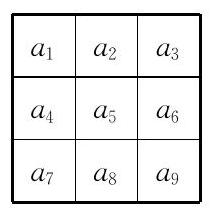
\includegraphics[max width=\textwidth, center]{2024_10_09_7e48ff928cc374c97394g-046(1)}

图 1\\
\begin{align}
& \left(a_{1}+a_{2}+a_{3}\right)+\left(a_{4}+a_{5}+a_{6}\right)+\left(a_{7}+a_{8}+a_{9}\right) \\
= & \left(a_{1}+a_{4}+a_{7}\right)+\left(a_{2}+a_{5}+a_{8}\right)+\left(a_{3}+a_{6}+a_{9}\right)
\end{align}

但此式左边为两奇一偶, 右边为 3 个奇数之和,导出左边为偶数,而右边为奇数,矛盾. 

所以,这 27 个和数中至多有 24 个数为奇数. \\
下面的例子(如图2所示)表明存在一种填数方式,使得 27 个和数中可以有 24 个为奇数. 图2各表中的 0 表示偶数, 1 表示奇数,从左到右依次为最上层, 中层和最下层的单位正方体. 

\begin{center}
\begin{tabular}{|l|l|l|}
\hline
0 & 1 & 0 \\
\hline
1 & 1 & 1 \\
\hline
0 & 1 & 0 \\
\hline
\end{tabular}
\end{center}

\begin{center}
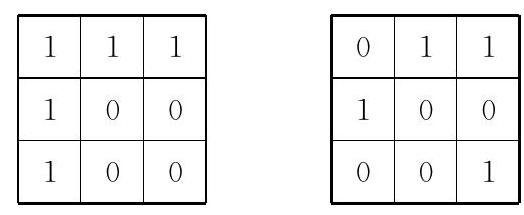
\includegraphics[max width=\textwidth]{2024_10_09_7e48ff928cc374c97394g-046}
\end{center}

图 2\\
所以,这 27 个和数中最多有 24 个为奇数.

\section{完全平方数}
数学竞赛中的许多问题涉及到完全平方数,需要用到完全平方数的一些特性. 

性质1 完全平方数 $\equiv 0$ 或 $1(\bmod 4)$ ,奇数的平方 $\equiv 1(\bmod 8)$ . \\
性质2 相邻两个完全平方数之间没有一个正整数是完全平方数. (这个性质经常用来证明某一类数不是完全平方数)

性质3 若两个互素的正整数之积是完全平方数,则这两个数都是完全平方数.

注意,"两个完全平方数之积是完全平方数"这个结论是显然的.\\
这里的性质2与性质3对一般的 $n$ 次方数都成立,而性质1只列出了完全平方数模 4 和模 8 的性质,模其余的数亦有一些相应的性质. 例如:完全平方数 $\equiv 0$ 或 $1(\bmod 3)$ ,完全平方数的末尾数字只能是 $0,1,4,5,6,9$ 等等. 

例1 设素数从小到大依次排列为 $p_{1}, p_{2}, \cdots$ . 证明:对任意大于 1 的正整数 $n$ ,数 $p_{1} p_{2} \cdots p_{n}-1$ 和 $p_{1} p_{2} \cdots p_{n}+1$ 都不是完全平方数. 

证明 注意到, $n \geqslant 2$ 时, $3 \mid p_{1} p_{2} \cdots p_{n}$, 故\\
\begin{align*}
p_{1} p_{2} \cdots p_{n}-1 \equiv 2(\bmod 3)
\end{align*}

所以, $p_{1} p_{2} \cdots p_{n}-1$ 不是完全平方数.\\
又 $n \geqslant 2$ 时, $p_{2} \cdots p_{n}$ 为奇数, 设 $p_{2} \cdots p_{n}=2 k+1$, 就有\\
\begin{align*}
p_{1} p_{2} \cdots p_{n}+1=2(2 k+1)+1=4 k+3 \equiv 3(\bmod 4)
\end{align*}

所以, $p_{1} p_{2} \cdots p_{n}+1$ 也不是完全平方数.\\
说明 在处理与完全平方数有关的问题时,经常要用到同余的方法,其中取恰当的"参照物"(即模哪个数)是非常关键的. 

例 2 已知正整数 $a ,  b$ 满足关系式\\
\begin{align*}
2 a^{2}+a=3 b^{2}+b
\end{align*}

证明: $a-b$ 和 $2 a+2 b+1$ 都是完全平方数.\\
证明 由条件,知\\
\begin{align*}
b^{2}=2 a^{2}+a-\left(2 b^{2}+b\right)=(a-b)(2 a+2 b+1)
\end{align*}

上式左边大于零,右边中 $2 a+2 b+1$ 大于零,故 $a-b$ 大于零. \\
由(1)知,要证 $a-b$ 与 $2 a+2 b+1$ 都是完全平方数,只需证明\\
\begin{align*}
(a-b, 2 a+2 b+1)=1
\end{align*}

设 $(a-b, 2 a+2 b+1)=d$ ,则由(1)知 $d^{2} \mid b^{2}$ ,故 $d \mid b$ . 进而结合 $d \mid a-b$ ,知 $d \mid a$ ,故 $d \mid 2(a+b)$.又 $d \mid 2 a+2 b+1$ ,所以, $d \mid 1$ ,进而 $d=1$.

命题获证.

说明 这里我们并没有求出(1)中 $a ,  b$ 的值(这是比较困难的),但是我们对(1)作恰当变形,使一边为完全平方数, 另一边是两个式子之积后,问题解决起来就容易了. 

例3 设正整数 $x ,  y ,  z$ 满足 $(x, y, z)=1$ ,并且 $\frac{1}{x}+\frac{1}{y}=\frac{1}{z}$. 证明: $x+y ,  x-z ,  y-z$ 都是完全平方数. 

证明 设 $(x, y)=m$ ,并设 $x=m n, y=m l$ ,这里 $m ,  l ,  n$ 都是正整数,且 $(l, n)=1$. 从而,由条件可知\\
\begin{align*}
(l+n) z=m l n
\end{align*}

利用 $(x, y, z)=1$ ,知 $(m, z)=1$ ,于是,由(1)知 $z \mid \ln$ . 而 $(l, n)=1$ ,故 $(l, l+n)=1,(n, l+n)=1$ ,因此,由(1)知 $l|z, n| z$ ,再由 $(l, n)=1$ ,知 $l n \mid z$ . 所以, $z=l n$ ,进而 $m=l+n$ . 这样,我们有\\
\begin{align*}
\begin{gathered}
x+y=m(l+n)=(l+n)^{2} \\
x-z=m n-l n=n(m-l)=n^{2} \\
y-z=m l-l n=l(m-n)=l^{2}
\end{gathered}
\end{align*}

命题获证.\\
说明 另一种处理方式基于下面的变形:\\
\begin{align}
\frac{x+y}{x y}=\frac{1}{z} & \Rightarrow \frac{x+y}{x}=\frac{y}{z} \\
& \Rightarrow \frac{x+y}{x}=\frac{x}{x-z} \\
& \Rightarrow(x+y)(x-z)=x^{2}
\end{align}

然后对最后一式利用上例的方法可证 $x+y$ 与 $x-z$ 都是完全平方数,这种处理或许更能体现问题的本质. 

例 4 求所有的素数 $p$ ,使得 $p^{3}-4 p+9$ 是一个完全平方数. \\
解 设 $p^{3}-4 p+9=x^{2}, x$ 为非负整数,则 $p \mid x^{2}-9$ ,即 $p \mid(x-3)(x+$ 3),结合 $p$ 为素数,可设 $x=k p \pm 3, k$ 为非负整数. 于是,\\
\begin{align*}
p^{3}-4 p=x^{2}-9=k^{2} p^{2} \pm 6 k p
\end{align*}

得 $p^{2}-4=k^{2} p \pm 6 k$ ,这表明: $p \mid 6 k \pm 4$ . \\
当 $p>2$ 时, $p$ 为奇素数, 可知 $p \mid 3 k \pm 2$, 故总有 $p \leqslant 3 k+2$, 这表明: $\frac{1}{3}\left(p^{2}-2 p-9\right) \leqslant p k-3 \leqslant x$.

若 $x \leqslant \frac{p^{2}}{4}$ ,则 $\frac{1}{3}\left(p^{2}-2 p-9\right) \leqslant \frac{p^{2}}{4}$ ,得 $p \leqslant 8+\frac{36}{p}$ ,可知 $p \leqslant 11$ ;\\
若 $x>\frac{p^{2}}{4}$, 则 $p^{3}-4 p+9=x^{2}>\frac{p^{4}}{16}$, 得 $p<16-\frac{16(4 p-9)}{p^{3}}$, 可知 $p \leqslant 13$.

综上可知, $p \leqslant 13$ ,直接枚举,得 $(p, x)=(2,3),(7,18),(11,36)$.求得 $p=2,7$ 或 11 .

说明 此例所处理的等式两边不是齐次的,想方设法得到素数 $p$ 的一个范围后去枚举是常用的方法, 这时一些数论知识的运用结合不等式估计往往是有效的. 

例5 已知 $n$ 为正整数,且 $2 n+1$ 与 $3 n+1$ 都是完全平方数. 证明: $40 \mid n$ . 证明 设 $2 n+1=x^{2}, 3 n+1=y^{2}$ ,其中 $x ,  y$ 都是正整数. \\
由性质1,知 $x^{2} \equiv 1(\bmod 8)$ (因为 $x^{2}$ 为奇数,故 $x$ 为奇数),从而\\
\begin{align*}
n \equiv 0(\bmod 4)
\end{align*}

进而 $3 n+1$ 为奇数,故

即\\
\begin{align*}
y^{2} \equiv 1(\bmod 8)
\end{align*}\\
\begin{align*}
3 n+1 \equiv 1(\bmod 8)
\end{align*}

于是\\
\begin{align*}
n \equiv 0(\bmod 8)
\end{align*}

另一方面,对任意整数 $a$ ,有\\
\begin{align*}
\begin{gathered}
a \equiv 0, \pm 1, \pm 2(\bmod 5) \\
a^{2} \equiv 0,1 \text { 或 } 4(\bmod 5) .
\end{gathered}
\end{align*}

故\\
由条件知 $x^{2}+y^{2}=5 n+2 \equiv 2(\bmod 5)$ ,\\
结合前面推出的结论,可知

故\\
从而\\
\begin{align*}
\begin{gathered}
x^{2} \equiv y^{2} \equiv 1(\bmod 5) \\
2 n+1 \equiv 1(\bmod 5) \\
n \equiv 0(\bmod 5)
\end{gathered}
\end{align*}

利用 $(5,8)=1$ ,可知 $40 \mid n$.\\
说明 最小的使得 $2 n+1$ 与 $3 n+1$ 都是完全平方数的正整数 $n=40$, 请读者找到下一个符合要求的正整数 $n$.

例 6 若 $a ,  b$ 是使得 $a b+1$ 为完全平方数的正整数,则记 $a \sim b$. 证明:若 $a \sim b$ ,则存在正整数 $c$ ,使得 $a \sim c, b \sim c$ . 

证明 由 $a \sim b$ ,可设 $a b+1=x^{2}$ ,这里 $x$ 为正整数,下一个与 $a ,  b ,  x$ 有关的完全平方数是 $(a+x)^{2}$ 或 $(b+x)^{2}$ ,于是,我们取 $c=2 x+a+b$ ,则\\
\begin{align}
a c+1 & =a(2 x+a+b)+1 \\
& =2 a x+a^{2}+a b+1 \\
& =2 a x+a^{2}+x^{2}=(x+a)^{2} \\
b c+1 & =(x+b)^{2}
\end{align}

命题获证.\\
说明 此题对代数式变形的能力要求较高. 在寻找完全平方数时,往往需要构造完全平方式,因为当一个整式中的字母都取整数时,这个整式的平方显然是完全平方数. 当然,反过来并不需要这样的条件. 

题中的 $c$ 还可以这样来找: 设 $a c+1=y^{2}$ ,则 $a(c-b)=y^{2}-x^{2}=(y-$ $x)(y+x)$ ,取 $y-x=a$ (此时 $c-b=y+x)$ 可符合此式,依此知应取 $c=b+$ $y+x=2 x+a+b$ . 

例 7 求所有的正整数数对 $(a, b)$, 使得\\
\begin{align*}
a^{3}+6 a b+1, b^{3}+6 a b+1
\end{align*}

都是完全立方数.\\
解 不妨设 $a \leqslant b$ ,则\\
\begin{align*}
b^{3}<b^{3}+6 a b+1 \leqslant b^{3}+6 b^{2}+1<(b+2)^{3}
\end{align*}

由 $b^{3}+6 a b+1$ 是一个完全立方数,可知\\
\begin{align*}
b^{3}+6 a b+1=(b+1)^{3}
\end{align*}

即有\\
\begin{align}
6 a b & =3 b^{2}+3 b \\
b & =2 a-1
\end{align}

从而\\
\begin{align*}
a^{3}+6 a b+1=a^{3}+12 a^{2}-6 a+1
\end{align*}

注意到 $\quad(a+1)^{3} \leqslant a^{3}+12 a^{2}-6 a+1<(a+4)^{3} ,$\\
因此, 由 $a^{3}+12 a^{2}-6 a+1$ 是完全立方数,可知只能是\\
\begin{align*}
a^{3}+12 a^{2}-6 a+1=(a+1)^{3},(a+2)^{3},(a+3)^{3} .
\end{align*}

分别求解,可得只能是 $a=1$.\\
所以,满足条件的数对 $(a, b)=(1,1)$ . \\
说明 先确定某个 $n$ 次方数夹在哪两个 $n$ 次方数之间,然后确定该 $n$ 次方数的取值. 这是用不等式估计处理问题的常见方法. 

例 8 求最小的正整数 $n$, 使得存在整数 $x_{1}, x_{2}, \cdots, x_{n}$ ,满足\\
\begin{align*}
x_{1}^{4}+x_{2}^{4}+\cdots+x_{n}^{4}=1599
\end{align*}

解 由性质1,对任意整数 $a ,$ 可知\\
\begin{align*}
a^{2} \equiv 0(\bmod 4) \text { 或 } a^{2} \equiv 1(\bmod 8),
\end{align*}

由此可得\\
\begin{align*}
a^{4} \equiv 0 \text { 或 } 1(\bmod 16) .
\end{align*}

利用这个结论,可知,若 $n<15$ ,设\\
\begin{align*}
x_{1}^{4}+x_{2}^{4}+\cdots+x_{n}^{4} \equiv m(\bmod 16)
\end{align*}

则\\
\begin{align*}
m \leqslant n<15
\end{align*}

而\\
\begin{align*}
1599 \equiv 15(\bmod 16)
\end{align*}

矛盾,所以\\
\begin{align*}
n \geqslant 15
\end{align*}

另外, 当 $n=15$ 时, 要求\\
\begin{align*}
x_{1}^{4} \equiv x_{2}^{4} \equiv \cdots \equiv x_{n}^{4} \equiv 1(\bmod 16)
\end{align*}

即 $x_{1}, x_{2}, \cdots, x_{n}$ 都为奇数,这为我们找到合适的数指明了方向. 事实上,在 $x_{1}, x_{2}, \cdots, x_{15}$ 中, 1 个数取为 5,12 个取为 3 ,另外两个取为 1 ,就有\\
\begin{align}
& x_{1}^{4}+x_{2}^{4}+\cdots+x_{15}^{4} \\
= & 5^{4}+12 \times 3^{4}+2 \\
= & 625+972+2 \\
= & 1599 .
\end{align}

所以, $n$ 的最小值为 15 .\\
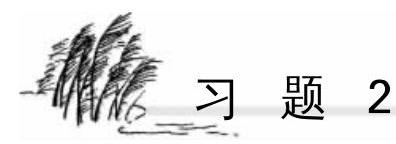
\includegraphics[max width=\textwidth, center]{2024_10_09_7e48ff928cc374c97394g-051}

1 设 $p ,  q$ 都是素数,且 $7 p+q, p q+11$ 也都为素数,求 $\left(p^{2}+q^{p}\right)\left(q^{2}+p^{q}\right)$的值. \\
2 设 $p_{1}<p_{2}<p_{3}<p_{4}<p_{5}$ 是 5 个素数,且 $p_{1}, p_{2}, p_{3}, p_{4}, p_{5}$ 成等差数列. 求 $p_{5}$ 的最小值.\\
3 对每个正整数 $n$ ,用 $S(n)$ 表示 $n$ 在十进制表示下各数码之和. 证明:对任意正整数 $m$ ,存在正整数 $n$ ,使得 $S(n)=m S(3 n)$ . \\
4 求最大的正整数 $k$ ,使得存在正整数 $n$ ,满足 $2^{k} \mid 3^{n}+1$ . 

5 设 $n$ 为正整数. 证明:存在十进制表示中只出现数码 0 和 1 的正整数 $m$ ,使得 $n \mid m$ . \\
6 设 $n$ 是一个正奇数. 证明:存在一个十进制表示中每个数码都是奇数的正整数 $m$ ,使得 $n \mid m$ . \\
7 证明:对每个正整数 $n$ ,数 $19 \times 8^{n}+17$ 都是合数. \\
8 Fibonaccia 数列 $\left\{F_{n}\right\}$ 定义如下: $F_{1}=F_{2}=1, F_{n+2}=F_{n+1}+F_{n}, n=1$ , $2, \cdots$\\
(1)证明:该数列任意连续 10 项之和是 11 的倍数;\\
(2)求最小的正整数 $k$ ,使得该数列中任意连续 $k$ 项之和是 12 的倍数. \\
9 设整数 $a ,  b$ 满足: $21 \mid a^{2}+b^{2}$ . 证明: $441 \mid a^{2}+b^{2}$ . \\
10 正整数 $a ,  b ,  c$ 满足: $c^{2}=a^{2}+b^{2}+a b$ . 证明: $c$ 有一个大于 5 的素因子. \\
11 将整数 $1,2, \cdots, 9$ 填入一个 $3 \times 3$ 的表格,每格一个数,使得每行, 每列及每条对角线上各数之和都是 9 的倍数. \\
(1)证明:该表格中正当中那个方格内的数是 3 的倍数;\\
(2)给出一个正当中方格内所填数为 6 的满足条件的放置方法.\\
12 下面的算式给出了一种判别一个数是否为 19 的倍数的方法:每次去掉该数的最后一位数字,将其两倍与剩下的数相加,依此类推,直到数变为 20以内的数为止,若最后一个数为 19 ,则最初的那个数为 19 的倍数,否则原数不是 19 的倍数. \\
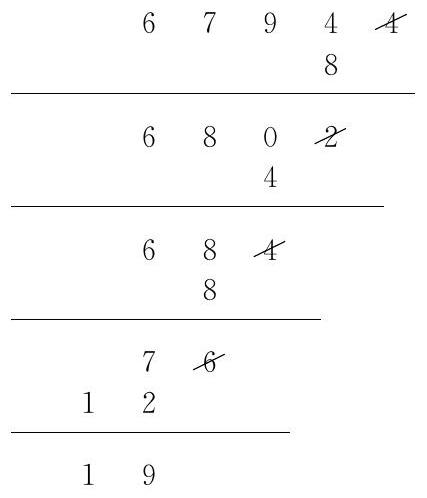
\includegraphics[max width=\textwidth, center]{2024_10_09_7e48ff928cc374c97394g-052}\\
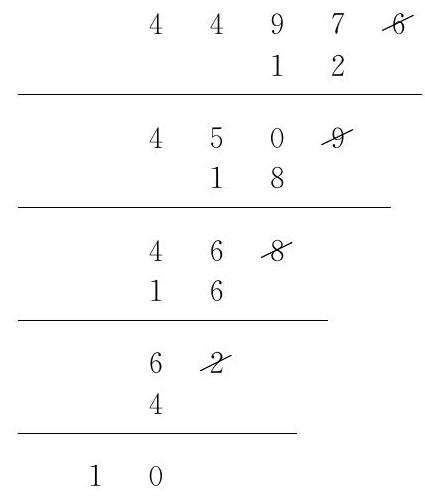
\includegraphics[max width=\textwidth, center]{2024_10_09_7e48ff928cc374c97394g-052(1)}

例如上面判定了 67944 为 19 的倍数,而 44976 不是 19 的倍数. \\
(1)试证明:上面的判别方法是正确的;\\
(2)请给出判别一个数是否为 29 的倍数的类似方法.\\
13 能否将 $2010 \times 2010$ 的方格表的每个方格染成黑色或白色,使得关于表格的中心对称的方格颜色不同,且每行, 每列中黑格数与白格数都各占一半?

14 标号为 $1,2, \cdots, 100$ 的火柴盒中有一些火柴,如果每次提问允许问其中任意 15 盒中所有火柴数之和的奇偶性. 那么要确定1号盒中火柴数的奇偶性,至少需要提问几次?\\
15 求所有的正整数 $n$ ,使得可以在一个 $n \times n$ 的方格表的每个方格内写上 +1或 -1 ,满足:每个标号为 +1 的方格的相邻格中恰有一个标号是 -1 ,而每个标号为 -1 的方格的相邻格中恰有一个标号是 +1 . \\
16 设 $a_{1}, a_{2}, \cdots, a_{100}$ 是 $1,2, \cdots, 100$ 的一个排列,令 $b_{i}=a_{1}+a_{2}+\cdots+a_{i}$ , $i=1,2, \cdots, 100$ ,记 $r_{i}$ 为 $b_{i}$ 除以 100 所得的余数. 证明: $r_{1}, r_{2}, \cdots, r_{100}$中至少有 11 个不同的数. \\
17 求所有满足下述条件的正整数 $a$ 的个数:存在非负整数 $x_{0}, x_{1}, x_{2}, \cdots$, $x_{2001}$ ,使得 $a^{x_{0}}=a^{x_{1}}+a^{x_{2}}+\cdots+a^{x_{2001}}$ . \\
18 设 $m ,  n$ 为正整数, $m>1$ . 证明: $m\left(2^{m}-1\right) \mid n$ 的充要条件是 $\left(2^{m}-1\right)^{2} \mid$ $2^{n}-1$.\\
19 设正整数 $a ,  b$ 互素, $p$ 为奇素数. 证明: $\left(a+b, \frac{a^{p}+b^{p}}{a+b}\right)=1$ 或 $p$.\\
20 求最小的正整数 $a$ ,使得对任意整数 $x$ ,都有 $65 \mid\left(5 x^{13}+13 x^{5}+9 a x\right)$ . \\
21 是否存在整数 $a ,  b ,  c$ ,使得方程\\
\begin{align*}
a x^{2}+b x+c=0 \text { 和 }(a+1) x^{2}+(b+1) x+(c+1)=0
\end{align*}

都有两个整数根?\\
22 求所有的正整数组 $(x, y, z, w)$ ,使得 $x!+y!+z!=w!$ . \\
23 求满足下述条件的整数数组 $(a, b)$ 的组数: $0 \leqslant a, b \leqslant 36$ ,且 $a^{2}+b^{2}=$ $0(\bmod 37)$ . \\
24 设 $m ,  n$ 为正整数,且 $m n \mid m^{2}+n^{2}+m$ . 证明: $m$ 是一个完全平方数. \\
25 证明:若正整数 $n$ 可以表示为三个正整数的平方和的形式,则 $n^{2}$ 也可以表示为三个正整数的平方和的形式. \\
26 求所有的正整数 $n$ ,使得 $n$ 的三次方根等于 $n$ 去掉最后三位数字后得到的正整数.\\
27 证明:存在无穷多个整数 $n$ ,使得数 $n ,  n+1 ,  n+2$ 都可以表示为两个整数 (不必不同)的平方和. 例如: $0=0^{2}+0^{2}, 1=0^{2}+1^{2}, 2=1^{2}+1^{2}$ ,故 $n=0$ 即为一个满足条件的整数. \\
28 求最小的正整数 $n$ ,使得在十进制表示下 $n^{3}$ 的末三位数字是 888 . \\
29 设正整数 $n>1$ ,证明:数 $2^{n}-1$ 既不是完全平方数,也不是完全立方数. \\
30 设 $a ,  b ,  c$ 为正整数,且 $\sqrt{a}+\sqrt{b}+\sqrt{c}$ 为整数. 证明: $a ,  b ,  c$ 都是完全平方数.

31 已知正整数 $c$ 是一个奇合数. 证明:存在正整数 $a$ ,使得 $a \leqslant \frac{c}{3}-1$ ,且 $(2 a-1)^{2}+8 c$ 是一个完全平方数.\\
32 设整数 $a ,  b$ 满足:对任意正整数 $n$ ,数 $2^{n} \cdot a+b$ 都是完全平方数. 证明: $a=0$.\\
33 求不能表示为 42 的正倍数与一个合数之和的最大正整数. \\
34 求一个正整数 $n$ ,使得数 $n, n+1, \cdots, n+20$ 中每个数都与 30030 不互素. \\
35 是否存在连续 13 个正整数,其中每个数都是 $2 ,  3 ,  5 ,  7 ,  11$ 中的某个数的倍数?连续 14 个呢?\\
36 设 $p$ 为素数, $a ,  n$ 都是正整数,且 $2^{p}+3^{p}=a^{n}$ . 证明: $n=1$ . \\
37 圆周上排列着 2000 个点,在某个点上标上数 1 ,按顺时针方向数两个点,在其上标数 2 , 再数 3 个点标数 3 , 依此继续, 标出数 $1,2, \cdots, 2000$. 这样,有些点上没有标数,有些点上所标的数不止一个. 问:被标上 2000 的那个点上所标的数中最小的是多少?\\
38 圆周上有 800 个点,依顺时针方向标号为 $1,2, \cdots, 800$ ,它们将圆周分为 800 个间隙. 现在选定某个点,将其染上红色,然后进行下述操作:如果第 $k$ 号点染成了红色,那么依顺时针方向转过 $k$ 个间隙,将所到达的点染成红色. 问:依此规则,圆周上最多有多少个点被染成了红色?证明你的结论. \\
39 设 $m$ 为正整数,且 $m \equiv 2(\bmod 4)$ . 证明:至多存在一对正整数 $(a, b)$ ,使得 $m=a b$ ,且 $0<a-b<\sqrt{5+4 \sqrt{4 m+1}}$ . \\
40 设 $n$ 是一个大于 10 的正整数,且 $n$ 的每个数码都为 $1 ,  3 ,  7$ 或 9 . 证明: $n$有一个大于 10 的素因子. \\
41 求所有的素数对 $(p, q)$ ,使得 $p q \mid p^{p}+q^{q}+1$ . \\
42 设 $f(n)=1+n+n^{2}+\cdots+n^{2010}$ . 证明:对任意整数 $m$ ,若 $2 \leqslant m \leqslant 2010$ ,则不存在正整数 $n$, 使得 $m \mid f(n)$.\\
43 是否存在整数 $x ,  y$ ,使得 $x^{2012}-2010=4 y^{2011}+4 y^{2010}+2011 y$ ?

\section{不定方程}
未知数个数多于方程个数的方程(或方程组)称为不定方程(或不定方程组),初等数论中仅讨论未知数取值为整数的情形. 这一单元主要讨论不定方程的求解问题中涉及的一些基本方法. 

不定方程溯源极古,早在 1700 多年前,古希腊数学家丢番图(Diophantus)就对不定方程做过许多研究,不定方程甚至被称为丢番图方程. 许多不定方程问题的解决十分困难,是对人类智力的一种挑战,例如历时 358 年方获解决的费马大定理就曾吸引无数优秀数学家为之付出毕生的精力. 面对挑战,人类表现出了极大的决心, 毅力和杰出的智慧. 

\section{一次不定方程(组)}
依未知数的次数可对不定方程分类,其中最简单的是一次不定方程. \\
设 $k \geqslant 2$ 为整数,我们称方程\\
\begin{align*}
a_{1} x_{1}+a_{2} x_{2}+\cdots+a_{k} x_{k}=c
\end{align*}

为一次不定方程,其中 $a_{1} ,  a_{2} ,  \cdots ,  a_{k} ,  c$ 均为整数,且 $a_{1} ,  a_{2} ,  \cdots ,  a_{k}$ 都不为零. 

并非每一个一次不定方程都会有整数解,一个很显然的必要条件是: $\left(a_{1}, a_{2}, \cdots, a_{k}\right) \mid c$ . 事实上,这个条件也是充分的. 我们重点讨论两个变量的不定方程\\
\begin{align*}
a x+b y=c
\end{align*}

其中 $a ,  b ,  c$ 为整数,且 $a ,  b$ 都不为零. \\
定理1 不定方程(2)有整数解的充要条件是 $(a, b) \mid c$ . \\
证明 必要性是显然的,而充分性可由贝祖定理得到. \\
事实上,由贝祖定理,知存在整数 $x_{0} ,  y_{0}$ ,使得 $a x_{0}+b y_{0}=(a, b)$ . 设 $c=(a, b) c_{1}$ ,则 $\left(c_{1} x_{0}, c_{1} y_{0}\right)$ 是(2)的解,充分性获证. 

定理2 设不定方程(2)有整数解 $\left(x_{0}, y_{0}\right)$ ,则(2)的所有整数解为\\
\begin{align*}
\left\{\begin{array}{l}
x=x_{0}+\frac{b}{(a, b)} t, \\
y=y_{0}-\frac{a}{(a, b)} t .
\end{array}(t \text { 为整数 })\right.
\end{align*}

证明 设 $(x, y)$ 是(2)的一组整数解,结合 $\left(x_{0}, y_{0}\right)$ 为(2)的解,可知\\
\begin{align*}
\left\{\begin{array}{l}
a x+b y=c \\
a x_{0}+b y_{0}=c
\end{array}\right.
\end{align*}

于是\\
\begin{align*}
a\left(x-x_{0}\right)+b\left(y-y_{0}\right)=0
\end{align*}

即\\
\begin{align*}
a\left(x-x_{0}\right)=b\left(y_{0}-y\right)
\end{align*}

故\\
\begin{align*}
b \mid a\left(x-x_{0}\right)
\end{align*}

因此\\
\begin{align*}
\left.\frac{b}{(a, b)} \right\rvert\, x-x_{0}
\end{align*}

可设\\
\begin{align*}
x-x_{0}=\frac{b}{(a, b)} t
\end{align*}

则\\
\begin{align*}
y-y_{0}=-\frac{a}{(a, b)} t
\end{align*}

其中 $t$ 为整数,这表明方程(2)的解具有形式(3).\\
反过来,由(3)决定的整数组( $x, y$ )是方程(2)的解可以直接代入(2)验证得到. 

所以,定理 2 成立. \\
说明 由(3)决定的整数组 $(x, y)$ 称为(2)的通解,而 $\left(x_{0}, y_{0}\right)$ 为(2)的特解.定理 2 也表明为求(2)的通解只需先求出(2)的一个特解,而特解可由辗转相除的方法逆算得到,因此(2)的所有解有通法求出. 

其余的一次不定方程或方程组都可以转化为求解二元一次不定方程. \\
例1 求不定方程\\
\begin{align*}
7 x+19 y=2012
\end{align*}

的正整数解的组数.\\
解 先求出(1)的一个特解.\\
\begin{align*}
x=\frac{1}{7}(2012-19 y)=287-3 y+\frac{1}{7}(3+2 y)
\end{align*}

故 $\frac{1}{7}(3+2 y)$ 为整数, 取 $y_{0}=2$, 则 $x_{0}=282$.\\
利用定理 2 的结论, 方程(1)的通解为\\
\begin{align*}
\left\{\begin{array}{l}
x=282-19 t, \\
y=2+7 t .
\end{array}\right.
\end{align*}

结合 $x>0, y>0$ 及 $t$ 为整数, 可解得 $0 \leqslant t \leqslant 14$.\\
所以, 方程 (1) 共有 15 组正整数解.\\
例2 设正整数 $a ,  b$ 互素. 证明: 不定方程\\
\begin{align*}
a x+b y=a b-a-b
\end{align*}

没有非负整数解.\\
证明 若存在非负整数对 $\left(x_{0}, y_{0}\right)$ 满足 (1), 则\\
\begin{align*}
a\left(x_{0}+1\right)+b\left(y_{0}+1\right)=a b
\end{align*}

那么, 应有\\
\begin{align*}
a \mid b\left(y_{0}+1\right)
\end{align*}

又\\
\begin{align*}
(a, b)=1
\end{align*}

故\\
\begin{align*}
a \mid y_{0}+1
\end{align*}

而 $a$ 与 $y_{0}+1$ 都是正整数, 故 $a \leqslant y_{0}+1$.\\
同理可证: $b \mid x_{0}+1$, 进而 $b \leqslant x_{0}+1$. 但这时, (2)的左边 $\geqslant a b+b a=$ $2 a b>$ (2) 的右边, 矛盾.

所以,(1)没有非负整数解.\\
例3 设正整数 $a ,  b$ 互素, 而正整数 $c$ 大于 $a b-a-b$. 证明: 不定方程\\
\begin{align*}
a x+b y=c
\end{align*}

有非负整数解.\\
证明 设(1)的通解为\\
\begin{align*}
\left\{\begin{array}{l}
x=x_{0}+b t, \\
y=y_{0}-a t
\end{array}(t \text { 为整数 })\right.
\end{align*}

其中 $\left(x_{0}, y_{0}\right)$ 为(1)的特解.\\
这样, 通过调节 $t$ 的值 (对 $x_{0}$ 作加上 $b$ 或减去 $b$ 的操作) 可找到(1)的一个解 $\left(x_{1}, y_{1}\right)$ ,使得 $0 \leqslant x_{1} \leqslant b-1$ ,则\\
\begin{align*}
b y_{1}=c-a x_{1}>a b-a-b-a x_{1} \geqslant a b-a-b-a(b-1)=-b
\end{align*}

故\\
\begin{align*}
y_{1}>-1,
\end{align*}

即\\
\begin{align*}
y_{1} \geqslant 0
\end{align*}

这表明 $\left(x_{1}, y_{1}\right)$ 是(1)的非负整数解,命题获证. \\
说明 上面的两个例子得到的结论给出了使得(1)有非负整数解的条件,说明了只要 $c$ 充分大(例如 $c \geqslant c_{0}$ 时),(1)就有非负整数解,并求出了 $c_{0}$ 的最小值(这个最小值为 $a b-a-b+1$ ). 这是一个有趣而富有挑战性的问题,当变量个数不小于 3 时, $c_{0}$ 的最小值还没有找到. 

例 4 求不定方程\\
\begin{align*}
x+2 y+3 z=2012
\end{align*}

的正整数解的组数.\\
解 设 $(x, y, z)$ 为(1)的正整数解, 则 $3 z \leqslant 2009$ ,即 $1 \leqslant z \leqslant 669$ ,分别可得\\
\begin{align*}
x+2 y=2009,2006, \cdots, 5
\end{align*}

对应地, $y$ 的取值范围分别是\\
\begin{align}
& 1 \leqslant y \leqslant 1004,1 \leqslant y \leqslant 1002,1 \leqslant y \leqslant 1001 \\
& 1 \leqslant y \leqslant 999, \cdots, 1 \leqslant y \leqslant 2
\end{align}

由于当 $y ,  z$ 确定后, $x$ 的值唯一确定,所以(1)的正整数解共有\\
\begin{align}
& (1004+1002)+(1001+999)+\cdots+(5+3)+2 \\
= & 2006+2000+\cdots+8+2 \\
= & \frac{1}{2}(2006+2) \times 335=336340
\end{align}

综上可知,共有 336340 组正整数解. \\
例 5 求所有的正整数数组 $\left(a_{1}, a_{2}, \cdots, a_{n}\right)$ ,使得\\
\begin{align*}
\left\{\begin{array}{l}
a_{1} \leqslant a_{2} \leqslant \cdots \leqslant a_{n} \\
a_{1}+a_{2}+\cdots+a_{n}=26 \\
a_{1}^{2}+a_{2}^{2}+\cdots+a_{n}^{2}=62 \\
a_{1}^{3}+a_{2}^{3}+\cdots+a_{n}^{3}=164
\end{array}\right.
\end{align*}

解 由 $a_{i}$ 都是正整数,而 $6^{3}=216>164$ ,知每个 $a_{i}$ 都不大于 5 . 我们设 $a_{1}, a_{2}, \cdots, a_{n}$ 中 $1,2,3,4,5$ 的个数分别为 $x_{1}, x_{2}, x_{3}, x_{4}, x_{5}$ ,则\\
\begin{align*}
\left\{\begin{array}{l}
x_{1}+x_{2}+x_{3}+x_{4}+x_{5}=n \\
x_{1}+2 x_{2}+3 x_{3}+4 x_{4}+5 x_{5}=26 \\
x_{1}+4 x_{2}+9 x_{3}+16 x_{4}+25 x_{5}=62 \\
x_{1}+8 x_{2}+27 x_{3}+64 x_{4}+125 x_{5}=164
\end{array}\right.
\end{align*}

其中 $x_{1}, x_{2}, x_{3}, x_{4}, x_{5}$ 都是非负整数.\\
先确定 $x_{1}, x_{2}, \cdots, x_{5}$ 的值,这等价于求一个不定方程组的非负整数解. \\
由(4)知 $x_{5} \leqslant 1$, 若 $x_{5}=1$, 则(3), (4)变为\\
\begin{align*}
\left\{\begin{array}{l}
x_{1}+4 x_{2}+9 x_{3}+16 x_{4}=37 \\
x_{1}+8 x_{2}+27 x_{3}+64 x_{4}=39
\end{array}\right.
\end{align*}

由 (6) - (5) 得\\
\begin{align*}
4 x_{2}+18 x_{3}+48 x_{4}=2
\end{align*}

这在 $x_{2} ,  x_{3} ,  x_{4}$ 为非负整数时不能成立,所以\\
\begin{align*}
x_{5}=0
\end{align*}

又由 (3) - (2) 得 $2 x_{2}+6 x_{3}+12 x_{4}=36$ ,

即\\
\begin{align*}
x_{2}+3 x_{3}+6 x_{4}=18
\end{align*}

由 (4) 一 (2) 得\\
\begin{align*}
x_{2}+4 x_{3}+10 x_{4}=23
\end{align*}

再由 (8) - (7) 得 $\quad x_{3}+4 x_{4}=5$,\\
故\\
\begin{align*}
\left(x_{3}, x_{4}\right)=(5,0),(1,1)
\end{align*}

进而可得\\
\begin{align*}
\left(x_{1}, x_{2}, x_{3}, x_{4}\right)=(5,3,5,0),(1,9,1,1)
\end{align*}

利用上述结论,可知\\
\begin{align}
& \left(a_{1}, a_{2}, \cdots, a_{n}\right) \\
= & (1,1,1,1,1,2,2,2,3,3,3,3,3) \\
& (1,2,2,2,2,2,2,2,2,2,3,4)
\end{align}

说明 上述两例中都用到了不等式估计的方法,并没有从不定方程(组)的通解出发来处理,解题过程中把握了问题的特点,因此较快地得到了解答.

例6 将所有分母不大于 99 的最简分数从小到大排列,求与 $\frac{17}{76}$ 相邻的两个数.

解 设 $\frac{q}{p}$ 与 $\frac{n}{m}$ 是与 $\frac{17}{76}$ 相邻的两个数,且\\
\begin{align*}
\frac{q}{p}<\frac{17}{76}<\frac{n}{m}
\end{align*}

其中 $p ,  q ,  m ,  n$ 为正整数, 则

于是\\
\begin{align}
& 17 p-76 q>0 \\
& 17 p-76 q \geqslant 1
\end{align}

先考虑 $17 p-76 q=1$ 中满足 $p \leqslant 99$ 且使 $p$ 最大的正整数解. 为此需先求它的一个特解,利用\\
\begin{align*}
p=\frac{1}{17}(76 q+1)=4 q+\frac{1}{17}(8 q+1)
\end{align*}

可得一个特解 $(p, q)=(9,2)$, 于是此不定方程的通解为\\
\begin{align*}
(p, q)=(9+76 t, 2+17 t)
\end{align*}\\
$t$ 为整数. 这时在条件 $p \leqslant 99$ 下, $p$ 最大为 85 ,此时 $q=19$ . \\
另一方面,由\\
\begin{align*}
\frac{17}{76}-\frac{q}{p}=\frac{17 p-76 q}{76 p}
\end{align*}

可知, 若 $17 p-76 q \geqslant 2$, 则\\
\begin{align*}
\frac{17}{76}-\frac{q}{p} \geqslant \frac{2}{76 p}=\frac{1}{38 p} \geqslant \frac{1}{38 \times 99}>\frac{1}{76 \times 85}=\frac{17}{76}-\frac{19}{85}
\end{align*}

所以,在所给条件下,比 $\frac{17}{76}$ 小且最接近它的数为 $\frac{19}{85}$ . \\
类似讨论, 可知 $\frac{n}{m}=\frac{15}{67}$ . \\
综上,这些分数的排列中与 $\frac{17}{76}$ 相邻的两个数是 $\frac{19}{85}$ 和 $\frac{15}{67}$.\\
说明 题中利用正整数不小于 1 这个显然的事实,转为求一次不定方程的正整数解是关键.

\section{2 不定方程的常用解法}
对于高次不定方程,求出其通解然后再讨论有时是不现实的,因为我们甚至还没有找到判别一个高次不定方程是否有解的统一方法,当然要求出通解就更难了. 或许正是因为没有统一的方法来处理高次不定方程,对具体的

问题往往有许多方法来处理,并且每一种方法都表现出一定的创造性,所以,高次不定方程的问题频繁地在数学竞赛中出现. 

当然,结合整除与同余的一些理论,求解高次不定方程也有一些常见的处理思路和解决办法. 

\section{一, 因式分解法}
将方程的一边变为常数,而含字母的一边可以进行因式分解,这样对常数进行素因数分解后,对比方程两边,考察各因式的每种取值情况就可将不定方程变为若干个方程组去求解. 这就是因式分解法处理不定方程的基本思路. 

例 1 求方程\\
\begin{align*}
x y-10(x+y)=1
\end{align*}

的整数解.\\
解 利用十字相乘,可将(1)变形为\\
\begin{align*}
(x-10)(y-10)=101
\end{align*}

而 101 为素数,故\\
\begin{align}
& (x-10, y-10) \\
= & (1,101),(101,1),(-1,-101),(-101,-1)
\end{align}

分别求解, 得方程的整数解为\\
\begin{align*}
(x, y)=(11,111),(111,11),(9,-91),(-91,9)
\end{align*}

例 2 是否存在整数 $x ,  y ,  z$, 使得\\
\begin{align*}
x^{4}+y^{4}+z^{4}=2 x^{2} y^{2}+2 y^{2} z^{2}+2 z^{2} x^{2}+24 ?
\end{align*}

解 若存在整数 $x ,  y ,  z$ 满足条件, 则\\
\begin{align}
-24 & =2 x^{2} y^{2}+2 y^{2} z^{2}+2 z^{2} x^{2}-\left(x^{4}+y^{4}+z^{4}\right) \\
& =-\left(x^{2}+y^{2}\right)^{2}+2\left(x^{2}+y^{2}\right) z^{2}-z^{4}+4 x^{2} y^{2} \\
& =-\left(x^{2}+y^{2}-z^{2}\right)^{2}+4 x^{2} y^{2} \\
& =\left(2 x y+x^{2}+y^{2}-z^{2}\right)\left(2 x y-x^{2}-y^{2}+z^{2}\right) \\
& =\left((x+y)^{2}-z^{2}\right)\left(z^{2}-(x-y)^{2}\right) \\
& =(x+y+z)(x+y-z)(z+x-y)(y+z-x)
\end{align}

这要求 -24 能表示为 4 个整数 $x+y+z, x+y-z, z+x-y, y+z-x$ 的乘积的形式,而这 4 个数中任意两个数之差都为偶数,故这 4 个数具有相同的

奇偶性, 由 -24 为偶数, 知它们都是偶数, 但这要求 $2^{4} \mid 24$, 矛盾.\\
所以,不存在符合要求的整数.\\
说明 熟悉海伦公式的读者可以一眼看穿问题的本质. 事实上, $S_{\triangle A B C}=$ $\frac{1}{4} \sqrt{(a+b+c)(a+b-c)(b+c-a)(c+a-b)}$, 其中 $a ,  b ,  c$ 为 $\triangle A B C$ 的三边长,这就是海伦公式. 根号里面的式子展开后就是 $2 a^{2} b^{2}+2 b^{2} c^{2}+2 c^{2} a^{2}-$ $a^{4}-b^{4}-c^{4}$ . 

例 3 求所有的正整数对 $(m, n)$, 使得\\
\begin{align*}
n^{5}+n^{4}=7^{m}-1
\end{align*}

解 将(1)移项后作因式分解,得\\
\begin{align}
7^{m} & =n^{5}+n^{4}+1=n^{5}+n^{4}+n^{3}-\left(n^{3}-1\right) \\
& =n^{3}\left(n^{2}+n+1\right)-(n-1)\left(n^{2}+n+1\right) \\
& =\left(n^{3}-n+1\right)\left(n^{2}+n+1\right)
\end{align}

由(1)知 $n>1$ ,而 $n=2$ 时,可得 $m=2$ . \\
下面考虑 $n>2$ 的情形,我们先看(2)式右边两个式子的最大公因数.\\
\begin{align}
& \left(n^{3}-n+1, n^{2}+n+1\right)=\left(n^{3}-n+1-\left(n^{2}+n+1\right)(n-1), n^{2}+n+1\right) \\
= & \left(-n+2, n^{2}+n+1\right)=\left(-n+2, n^{2}+n+1+(-n+2)(n+3)\right) \\
= & (-n+2,7)
\end{align}

故 $\left(n^{3}-n+1, n^{2}+n+1\right) \mid 7$.\\
结合(2)式知 $n^{3}-n+1$ 与 $n^{2}+n+1$ 都是 7 的幂次, 而它们在 $n \geqslant 3$ 时, 都大于 7 , 这导致 $7^{2} \mid\left(n^{3}-n+1, n^{2}+n+1\right)$ ,与前所得矛盾.

综上可知, 只有 $(m, n)=(2,2)$ 符合要求.\\
说明 对(1)式变形后, 所得(2)式两边符合因式分解方法解不定方程的套路, 但 $7^{m}$ 并不是一个常数, 这里需要有另外的方法来处理才能继续下去. 活学活用方能攻城拔寨. 

\section{二, 配方法}
配方是代数变形中的常见方法, 在处理不定方程的问题时还可综合利用完全平方数的特性, 因此配方法在求解不定方程时大有用武之地.

例 4 求不定方程 $3 x^{2}-4 x y+3 y^{2}=35$ 的全部整数解. \\
解 对方程两边都乘以 3 , 配方后即得\\
\begin{align*}
(3 x-2 y)^{2}+5 y^{2}=105
\end{align*}

由(1)式得\\
所以\\
\begin{align*}
5 y^{2} \leqslant 105
\end{align*}\\
\begin{align*}
|y| \leqslant 4
\end{align*}

当 $|y|=4$ 时, $|3 x-2 y|=5$ ,此时原方程的解为\\
\begin{align*}
(x, y)=(1,4),(-1,-4)
\end{align*}

当 $|y|=1$ 时, $|3 x-2 y|=10$ ,此时原方程的解为\\
\begin{align*}
(x, y)=(4,1),(-4,-1)
\end{align*}

当 $|y|=0,2,3$ 时, $(3 x-2 y)^{2}$ 分别为 $105,85,60$. 此时, 所得的方程组显然无整数解.

上面的讨论表明,原方程有 4 组解:\\
\begin{align*}
(x, y)=(4,1),(1,4),(-4,-1),(-1,-4)
\end{align*}

例 5 求方程 $x^{2}+x=y^{4}+y^{3}+y^{2}+y$ 的整数解. \\
解 同上例,对方程两边同乘以 4 ,并对左边进行配方,得\\
\begin{align*}
(2 x+1)^{2}=4\left(y^{4}+y^{3}+y^{2}+y\right)+1
\end{align*}

下面对(1)式右端进行估计. 由于\\
\begin{align}
& 4\left(y^{4}+y^{3}+y^{2}+y\right)+1 \\
= & \left(2 y^{2}+y+1\right)^{2}-y^{2}+2 y \\
= & \left(2 y^{2}+y\right)^{2}+3 y^{2}+4 y+1,
\end{align}

从而,当 $y>2$ 或 $y<-1$ 时,有\\
\begin{align*}
\left(2 y^{2}+y\right)^{2}<(2 x+1)^{2}<\left(2 y^{2}+y+1\right)^{2}
\end{align*}

由于 $2 y^{2}+y$ 与 $2 y^{2}+y+1$ 是两个连续的整数,它们的平方之间不会含有完全平方数,故上式不成立. 

因此只需考虑当 $-1 \leqslant y \leqslant 2$ 时方程的解,这是平凡的,容易得到原方程的全部整数解是\\
\begin{align*}
(x, y)=(0,-1),(-1,-1),(0,0),(-1,0),(-6,2),(5,2)
\end{align*}

例 6 求所有的正整数 $n \geqslant 2$, 使得不定方程组\\
\begin{align*}
\left\{\begin{array}{c}
x_{1}^{2}+x_{2}^{2}+50=16 x_{1}+12 x_{2} \\
x_{2}^{2}+x_{3}^{2}+50=16 x_{2}+12 x_{3} \\
\cdots \\
x_{n-1}^{2}+x_{n}^{2}+50=16 x_{n-1}+12 x_{n} \\
x_{n}^{2}+x_{1}^{2}+50=16 x_{n}+12 x_{1}
\end{array}\right.
\end{align*}

有整数解.\\
解 移项后配方,方程组变形为\\
\begin{align*}
\left\{\begin{array}{c}
\left(x_{1}-8\right)^{2}+\left(x_{2}-6\right)^{2}=50 \\
\left(x_{2}-8\right)^{2}+\left(x_{3}-6\right)^{2}=50 \\
\cdots \\
\left(x_{n-1}-8\right)^{2}+\left(x_{n}-6\right)^{2}=50 \\
\left(x_{n}-8\right)^{2}+\left(x_{1}-6\right)^{2}=50
\end{array}\right.
\end{align*}

由于 50 表示为两个正整数的平方和只有两种: $50=1^{2}+7^{2}=5^{2}+5^{2}$, 所以,由(1)知 $\left|x_{2}-6\right|=1 ,  5$ 或 7,而由(2)知 $\left|x_{2}-8\right|=1 ,  5$ 或 7, 从而 $x_{2}=1$ ,  7 或 13 . 

进一步,可知对每个 $1 \leqslant i \leqslant n$ ,都有 $x_{i}=1,7$ 或 13 ,依 $x_{1}=1 ,  7 ,  13$ ,分三种情况讨论. 

若 $x_{1}=1$,则由(1)知 $x_{2}=7$, 再由 (2)知 $x_{3}=13$, 依次往下递推, 可知当 $k \equiv 1(\bmod 3)$ 时, $x_{k}=1$ ;当 $k \equiv 2(\bmod 3)$ 时, $x_{k}=7$ ;当 $k \equiv 0(\bmod 3)$ 时, $x_{k}=13$. 所以, 由第 (2) 式, 知当且仅当 $n+1 \equiv 1(\bmod 3)$ 时, 原方程组有整数解, 即当且仅当 $3 \mid n$ 时, $n$ 符合要求.

对另外两种情况 $x_{1}=7$ 和 $x_{1}=13$ 同样讨论, 得到的条件是一样的.\\
综上可知,满足条件的 $n$ 是所有 3 的倍数. \\
说明 进一步讨论可知,当 $3 \mid n$ 时,方程组恰有 3 组整数解. 

\section{三, 不等式估计}
利用不等式的知识, 先确定不定方程中的某个字母的范围, 然后逐个枚举得到所有解,这个方法称为不等式估计,它也是我们处理不定方程的常见方法. 当然, 如果能够恰当地利用字母的对称性等, 那么作不等式估计时会简洁很多. 

例 7 求不定方程 $x^{3}-y^{3}=x y+61$ 的正整数解.\\
解 设 $(x, y)$ 为方程的正整数解, 则 $x>y$. 设 $x=y+d$, 则 $d$ 为正整数, 且\\
\begin{align}
(y+d) y+61 & =(y+d)^{3}-y^{3} \\
& =3 d y^{2}+3 y d^{2}+d^{3}
\end{align}

即有\\
\begin{align*}
(3 d-1) y^{2}+d(3 d-1) y+d^{3}=61
\end{align*}

故\\
\begin{align*}
d^{3}<61
\end{align*}

于是\\
\begin{align*}
d \leqslant 3
\end{align*}

分别令 $d=1 ,  2 ,  3$ 代入, 得\\
\begin{align}
& 2 y^{2}+2 y+1=61 \\
& 5 y^{2}+10 y+8=61 \\
& 8 y^{2}+24 y+27=61
\end{align}

只有第一个方程有整数解, 并由 $y$ 为正整数知 $y=5$, 进而 $x=6$.\\
所以, 原方程只有一组正整数解 $(x, y)=(6,5)$.\\
例 8 求所有的正整数 $a ,  b$, 使得\\
\begin{align*}
4^{a}+4 a^{2}+4=b^{2}
\end{align*}

解 若 $(a ,  b)$ 是满足(1) 的正整数数对, 则 $b^{2}$ 为偶数, 且 $b^{2}>4^{a}$, 从而 $b$ 为偶数, 且 $b>2^{a}$, 故 $b \geqslant 2^{a}+2$. 于是\\
\begin{align*}
4^{a}+4 a^{2}+4=b^{2} \geqslant\left(2^{a}+2\right)^{2}=4^{a}+4 \cdot 2^{a}+4
\end{align*}

知 $a^{2} \geqslant 2^{a}$, 可得 $a \leqslant 4$ (对 $a$ 归纳可证: 当 $a \geqslant 5$ 时, 有 $a^{2}<2^{a}$ ).\\
分别就 $a=1,2,3,4$ 代入 (1) 式, 可得方程的所有正整数解为 $(a, b)=$ $(2,6)$ 或 $(4,18)$.

例 9 求所有的正整数数组 $(a, b, c, x, y, z)$, 使得\\
\begin{align*}
\left\{\begin{array}{l}
a+b+c=x y z \\
x+y+z=a b c
\end{array}\right.
\end{align*}

这里 $a \geqslant b \geqslant c, x \geqslant y \geqslant z$.\\
解 由对称性,我们只需考虑 $x \geqslant a$ 的情形. 这时\\
\begin{align*}
x y z=a+b+c \leqslant 3 a \leqslant 3 x
\end{align*}

故\\
\begin{align*}
y z \leqslant 3
\end{align*}

于是\\
\begin{align*}
(y, z)=(1,1),(2,1),(3,1)
\end{align*}

当 $(y, z)=(1,1)$ 时, $a+b+c=x$ 且 $x+2=a b c$, 于是\\
\begin{align*}
a b c=a+b+c+2 .
\end{align*}

若 $c \geqslant 2$, 则\\
\begin{align*}
a+b+c+2 \leqslant 3 a+2 \leqslant 4 a \leqslant a b c,
\end{align*}

等号当且仅当 $a=b=c=2$ 时成立.\\
若 $c=1$, 则\\
\begin{align*}
a b=a+b+3
\end{align*}

即\\
\begin{align*}
(a-1)(b-1)=4
\end{align*}

得\\
\begin{align*}
(a, b)=(5,2),(3,3)
\end{align*}

当 $(y, z)=(2,1)$ 时, $2 a b c=2 x+6=a+b+c+6$ ,与上述类似讨论可知 $c=1$ ,进而

得\\
\begin{align*}
\begin{gathered}
(2 a-1)(2 b-1)=15 \\
(a, b)=(3,2)
\end{gathered}
\end{align*}

当 $(y, z)=(3,1)$ 时, $3 a b c=3 x+12=a+b+c+12$, 类似可知,此时无解.

综上所述, 可知\\
\begin{align}
& (a, b, c, x, y, z) \\
= & (2,2,2,6,1,1),(5,2,1,8,1,1),(3,3,1,7,1,1) \\
& (3,2,1,3,2,1),(6,1,1,2,2,2),(8,1,1,5,2,1) \\
& (7,1,1,3,3,1)
\end{align}

说明 此题中如果没有条件 $a \geqslant b \geqslant c$ 和 $x \geqslant y \geqslant z$ ,也需要利用对称性作出这样的假设后再处理,解题中利用对称性假设 $x \geqslant a$ 是巧妙的,这样问题就转化为只有 3 种情况而便于处理了. 

\section{四, 同余方法}
若不定方程 $F\left(x_{1}, x_{2}, \cdots, x_{n}\right)=0$ 有整数解,则对任意的 $m \in \mathbf{N}^{*}$ ,其整数解 $\left(x_{1}, x_{2}, \cdots, x_{n}\right)$ 均满足\\
\begin{align*}
F\left(x_{1}, x_{2}, \cdots, x_{n}\right) \equiv 0(\bmod m)
\end{align*}

运用这一条件,同余可以作为不定方程是否有整数解的一块试金石. \\
例 10 证明:不定方程\\
\begin{align*}
x^{2}+y^{2}-8 z^{3}=6
\end{align*}

没有整数解.\\
证明 若 $(x, y, z)$ 是方程(1)的整数解,对(1)的两边模2,可知 $x ,  y$ 同奇偶;再对(1)两边模 4 可知 $x ,  y$ 都为奇数,于是 $x^{2} \equiv y^{2} \equiv 1(\bmod 8)$ ,这要求\\
\begin{align*}
6=x^{2}+y^{2}-8 z^{3} \equiv 2(\bmod 8)
\end{align*}

矛盾. 故方程(1)没有整数解.\\
说明 利用同余方法解不定方程问题时,选择恰当的数作为模是十分重

要的, 它不仅涉及问题解决的繁简程度, 重要的是能否卡住字母的范围或导出矛盾.

例 11 求所有的非负整数 $x ,  y ,  z$, 使得\\
\begin{align*}
2^{x}+3^{y}=z^{2}
\end{align*}

解 (1) 当 $y=0$ 时, 有

于是可设\\
\begin{align*}
2^{x}=z^{2}-1=(z-1)(z+1)
\end{align*}

因此\\
\begin{align*}
z-1=2^{\alpha}, z+1=2^{\beta}, 0 \leqslant \alpha \leqslant \beta,
\end{align*}\\
\begin{align*}
2^{\beta}-2^{\alpha}=2
\end{align*}

此时, 若 $\alpha \geqslant 2$, 则 $4 \mid 2^{\beta}-2^{\alpha}$, 与 $4 \nmid 2$ 矛盾, 故 $\alpha \leqslant 1$. 而 $\alpha=0$ 导致 $2^{\beta}=$ 3 , 矛盾,故

所以\\
\begin{align}
& \alpha=1, \beta=2 \\
& z=3, x=3
\end{align}

得\\
\begin{align*}
(x, y, z)=(3,0,3)
\end{align*}\\
(2) 当 $y>0$ 时, 由于 $3 \nmid 2^{x}+3^{y}$, 故 $3 \nmid z$, 所以\\
\begin{align*}
z^{2} \equiv 1(\bmod 3)
\end{align*}

对(1)两边模 3 ,知\\
\begin{align*}
(-1)^{x} \equiv 1(\bmod 3)
\end{align*}

故 $x$ 为偶数, 现在设 $x=2 m$, 则\\
\begin{align*}
\left(z-2^{m}\right)\left(z+2^{m}\right)=3^{y}
\end{align*}

所以可设\\
\begin{align*}
z-2^{m}=3^{\alpha}, z+2^{m}=3^{\beta}, 0 \leqslant \alpha \leqslant \beta, \alpha+\beta=y
\end{align*}

于是\\
\begin{align*}
3^{\beta}-3^{\alpha}=2^{m+1},
\end{align*}

若 $\alpha \geqslant 1$, 则 $3 \mid 3^{\beta}-3^{\alpha}$, 但 $3 \nmid 2^{m+1}$, 矛盾, 故 $\alpha=0$, 因此\\
\begin{align*}
3^{\beta}-1=2^{m+1}
\end{align*}

当 $m=0$ 时, $\beta=1$, 得\\
\begin{align*}
(x, y, z)=(0,1,2)
\end{align*}

当 $m>0$ 时, $2^{m+1} \equiv 0(\bmod 4)$ ,故\\
\begin{align*}
3^{\beta} \equiv 1(\bmod 4)
\end{align*}

这要求 $\beta$ 为偶数,设 $\beta=2 n$ ,则\\
\begin{align*}
2^{m+1}=3^{2 n}-1=\left(3^{n}-1\right)\left(3^{n}+1\right)
\end{align*}

同 $y=0$ 时的讨论,可知 $\quad 3^{n}-1=2$ ,\\
即 $n=1$ ,进而 $m=2$ ,得\\
\begin{align*}
(x, y, z)=(4,2,5)
\end{align*}

所以 $(x, y, z)=(3,0,3),(0,1,2),(4,2,5)$.\\
例 12 设 $m ,  n$ 为正整数,且 $n>1$. 求 $\left|2^{m}-5^{n}\right|$ 的最小值.\\
解 由于 $\left|2^{m}-5^{n}\right|$ 为奇数,而 $m=7, n=3$ 时, $\left|2^{m}-5^{n}\right|=3$ ,故若能证明 $n>1$ 时, $\left|2^{m}-5^{n}\right| \neq 1$ ,则所求的最小值为 3 . 

若存在正整数 $m ,  n$, 使得 $n>1$, 且 $\left|2^{m}-5^{n}\right|=1$, 则\\
\begin{align*}
2^{m}-5^{n}=1 \text { 或 } 2^{m}-5^{n}=-1
\end{align*}

如果 $2^{m}-5^{n}=1$, 那么 $m \geqslant 3$ ,两边模 8 ,要求\\
\begin{align*}
5^{n} \equiv 7(\bmod 8)
\end{align*}

但对任意正整数 $n, 5^{n} \equiv 1$ 或 $5(\bmod 8)$ ,矛盾,故 $2^{m}-5^{n}=1$ 不成立. \\
如果 $2^{m}-5^{n}=-1$, 那么由 $n>1$, 知 $m \geqslant 3$ . 两边模 8 , 得\\
\begin{align*}
5^{n} \equiv 1(\bmod 8)
\end{align*}

可知 $n$ 为偶数. 设 $n=2 x, x$ 为正整数,则\\
\begin{align*}
2^{m}=\left(5^{x}-1\right)\left(5^{x}+1\right)
\end{align*}

由于 $5^{x}-1$ 与 $5^{x}+1$ 是两个相邻偶数, 这要求\\
\begin{align*}
5^{x}-1=2,5^{x}+1=4
\end{align*}

不可能.\\
所以, $\left|2^{m}-5^{n}\right|$ 的最小值为 3 . \\
说明 上面的两个例子都用到了一个结论:两个差为 2 的正整数之积为 2的幂次,则这两个数只能为 2 和 4 . 该结论在例 11 的前半段解答中已予以证明.

\section{五, 构造法}
有些不定方程的问题只需证明该方程有解或有无穷多个解,这时经常采用构造法来处理. 

例13 证明:方程 $x^{2}+y^{5}=z^{3}$ 有无穷多组满足 $x y z \neq 0$ 的整数解. \\
证明 取 $x=2^{15 k+10}, y=2^{6 k+4}, z=2^{10 k+7}, k$ 为非负整数,则这样的 $x$ ,  $y ,  z$ 满足 $x^{2}+y^{5}=z^{3}$ ,所以方程有无穷多组满足 $x y z \neq 0$ 的整数解. 

另证 先求方程的一组特解,易知 $x=10 , y=3 , z=7$ 是方程 $x^{2}+$ $y^{5}=z^{3}$ 的一组解. 因而 $x=10 a^{15 k}, y=3 a^{6 k}, z=7 a^{10 k}(a, k$ 为非负整数) 是方程的解. 

例14 证明:对任意整数 $n$ ,方程\\
\begin{align*}
x^{2}+y^{2}-z^{2}=n
\end{align*}

有无穷多组整数解( $x, y, z)$ . \\
证明 现有命题"当 $m$ 为奇数或 4 的倍数时,方程 $a^{2}-b^{2}=m$ 有整数解 $(a, b)$ ", 它对解决本题是有用的. 这个命题基于下面 2 个恒等式:\\
\begin{align*}
\begin{gathered}
(k+1)^{2}-k^{2}=2 k+1 \\
(k+1)^{2}-(k-1)^{2}=4 k
\end{gathered}
\end{align*}

对于方程 (1),只需取 $x$ ,使 $x$ 与 $n$ 的奇偶性相反(这样的 $x$ 有无穷多个),从而利用上述命题,方程\\
\begin{align*}
y^{2}-z^{2}=n-x^{2}
\end{align*}

有整数解,可知方程(1)有无穷多组整数解. \\
例15 是否存在两两不同的正整数 $m ,  n ,  p ,  q$, 使得 $m+n=p+q$ 和 $\sqrt{m}+\sqrt[3]{n}=\sqrt{p}+\sqrt[3]{q}>2012$ 都成立?

解 存在满足条件的正整数. \\
由方程的结构,我们寻找形如\\
\begin{align*}
m=a^{2}, n=b^{3}, p=c^{2}, q=d^{3}
\end{align*}

的正整数. 这里 $a ,  b ,  c ,  d$ 为正整数. \\
此时, 条件转化为\\
\begin{align*}
a+b=c+d>2012, a^{2}+b^{3}=c^{2}+d^{3}
\end{align*}

即\\
\begin{align*}
a-c=d-b,(a-c)(a+c)=(d-b)\left(d^{2}+b d+b^{2}\right)
\end{align*}

令 $d-b=1$ ,即 $b=d-1$ ,且使 $b>2012$ ,则 $b ,  d$ 的奇偶性不同,现令\\
\begin{align*}
a=\frac{b^{2}+b d+d^{2}+1}{2}, c=\frac{b^{2}+b d+d^{2}-1}{2}
\end{align*}

那么 $a ,  c$ 为正整数,且由 $a ,  b ,  c ,  d$ 确定的 $m ,  n ,  p ,  q$ 满足条件.

例16 证明:存在无穷多组正整数组( $x, y, z$ ),使得 $x, y, z$ 两两不同,并且\\
\begin{align*}
x^{x}=y^{3}+z^{3}
\end{align*}

证明 一个想法是:将 $x$ 取为 $3 k+1$ 形式的数,这时\\
\begin{align}
x^{x} & =(3 k+1)^{3 k+1} \\
& =(3 k+1)(3 k+1)^{3 k} \\
& =3 k(3 k+1)^{3 k}+(3 k+1)^{3 k}
\end{align}

因此,如果使 $3 k$ 为一个完全立方数, 那么符合要求的正整数 $x ,  y ,  z$ 就找到了. 

为此, 令 $k=3^{3 m+2}$, 这里 $m$ 为正整数, 那么令\\
\begin{align*}
x=3 k+1, y=3^{m+1}(3 k+1)^{k}, z=(3 k+1)^{k}
\end{align*}

则 $x ,  y ,  z$ 两两不同,且满足 $x^{x}=y^{3}+z^{3}$ . 命题获证. \\
说明 如果不要求 $x ,  y ,  z$ 两两不同,我们还可以这样来构造:取 $y=$ $z=2^{m} , x=2^{\alpha}$ ,则当 $\alpha \cdot 2^{\alpha}=3 m+1$ 时,就有 $x^{x}=y^{3}+z^{3}$ . 容易看出满足 $\alpha \cdot 2^{\alpha}=3 m+1$ 的正整数对 $(\alpha, m)$ 有无穷多对. 

\section{3 勾股方程}
在我国古代算书《周髀算经》(公元前 1 世纪)中就有"勾广三, 股修四, 经隅五"的记载,这是关于勾股数的早期记录. 

所谓勾股数是指满足下述方程\\
\begin{align*}
x^{2}+y^{2}=z^{2}
\end{align*}

的正整数数组.\\
方程(1)称为勾股方程(英文著作中,该方程称为毕达哥拉斯(Pythagoras)方程,勾股定理亦称为毕达哥拉斯定理),讨论(1)的正整数解是二次不定方程中的一个重要课题,求解过程本身就有一定的挑战性. 

注意到,对(1)的解 $(x, y, z)$ ,如果 $(x, y)=d$ ,那么 $d^{2} \mid z^{2}$ ,即有 $d \mid z$ ,因此可以在(1)的两边约去 $d$ 后再讨论. 这说明我们只需在条件 $(x, y)=1$下,求(1)的所有正整数解. 易知当 $(x, y)=1$ 时, $x ,  y ,  z$ 两两互素,我们称(1)的使得 $x ,  y ,  z$ 两两互素的正整数解 $(x, y, z)$ 为本原勾股数组.

下面来求(1)的所有本原勾股数组. \\
设 $(x, y, z)$ 是 (1) 的一个本原解 (即 $(x, y, z)$ 是本原勾股数组), 则由\\
$(x, y)=1$ ,知 $x ,  y$ 不同为偶数. 若 $x ,  y$ 都是奇数,则 $z^{2}=x^{2}+y^{2} \equiv 1+$ $1=2(\bmod 4)$ ,这与完全平方数 $\equiv 0$ 或 $1(\bmod 4)$ 矛盾. 所以 $x ,  y$ 不同为奇数,即 $x ,  y$ 是一奇一偶. 

不妨设 $y$ 为偶数,则 $x ,  z$ 都是奇数,由(1)得

故\\
\begin{align*}
\begin{gathered}
y^{2}=z^{2}-x^{2} \\
\left(\frac{y}{2}\right)^{2}=\frac{z-x}{2} \cdot \frac{z+x}{2}
\end{gathered}
\end{align*}

由于\\
\begin{align}
\left(\frac{z-x}{2}, \frac{z+x}{2}\right) & =\left(\frac{z-x}{2}, \frac{z+x}{2}+\frac{z-x}{2}\right) \\
& =\left(\frac{z-x}{2}, z\right)=(z-x, z) \\
& =(x, z)=1
\end{align}

可知 $\frac{z-x}{2}$ 与 $\frac{z+x}{2}$ 都是完全平方数,所以,可设\\
\begin{align*}
\begin{gathered}
\left(\frac{z-x}{2}, \frac{z+x}{2}\right)=\left(m^{2}, n^{2}\right) \\
y=2 m n
\end{gathered}
\end{align*}

依此得\\
进一步,由 $\left(\frac{z-x}{2}, \frac{z+x}{2}\right)=1$ ,可知 $(m, n)=1$ ,而由 $x ,  z$ 都是奇数,知 $m, n$ 一奇一偶.

综上可知,(1)的所有本原解为\\
\begin{align*}
\left\{\begin{array} { l } 
{ x = n ^ { 2 } - m ^ { 2 } , } \\
{ y = 2 m n , } \\
{ z = m ^ { 2 } + n ^ { 2 } , }
\end{array} \text { 或 } \quad \left\{\begin{array}{l}
x=2 m n, \\
y=n^{2}-m^{2}, \\
z=m^{2}+n^{2},
\end{array}\right.\right.
\end{align*}

其中 $m ,  n$ 为正整数, $m<n$, 且 $(m, n)=1, m ,  n$ 一奇一偶.\\
注意 由(2)得到的正整数组 $(x, y, z)$ 代入验证,可知是(1)的解. 将(2)中的 $x ,  y ,  z$ 都乘以整数 $d$ 就可得(1)的全部整数解.

例1 设 $(x, y, z)$ 是勾股方程(1)的整数解. 证明: $x ,  y ,  z$ 中必有一个数是 3 的倍数,必有一个数是 4 的倍数,必有一个数是 5 的倍数. 

证明 利用完全平方数 $\equiv 0,1(\bmod 3)$ 知,若 $x ,  y$ 都不是 3 的倍数,则\\
\begin{align*}
x^{2}+y^{2} \equiv 2(\bmod 3)
\end{align*}

这导致\\
\begin{align*}
z^{2} \equiv 2(\bmod 3)
\end{align*}

矛盾. 故 $x ,  y$ 中有一个数是 3 的倍数.

若 $x ,  y ,  z$ 都不是 5 的倍数,则\\
\begin{align*}
x^{2}+y^{2} \equiv 0,2 \text { 或 } 3(\bmod 5),
\end{align*}

而\\
\begin{align*}
z^{2} \equiv 1 \text { 或 } 4(\bmod 5) ,
\end{align*}

矛盾. 故 $x ,  y ,  z$ 中有一个为 5 的倍数. \\
若 $x ,  y ,  z$ 都是偶数,则在(1)的两边同除以 4 ,直至 $x ,  y$ 中有一个为奇数,设 $x$ 为奇数,则 $y$ 必为偶数(否则 $z^{2}=x^{2}+y^{2} \equiv 1+1 \equiv 2(\bmod 4)$ ,矛盾),此时 $z$ 为奇数. 对(1)的两边模 8 ,可知 $y^{2} \equiv 0(\bmod 8)$ ,故 $4 \mid y$ . 

综上可知,命题成立. \\
说明 这里并不是说 $x ,  y ,  z$ 分别是 3,  $4 ,  5$ 的倍数(例如勾股数组 $(5,12,13)$ 中,是 3 的倍数与 4 的倍数的那个数是同一个数). 另外,如果从 (2)出发, 证明此题的结论会简便一些. 

例2 设 $(x, y, z)$ 是一组勾股数 $\left(x^{2}+y^{2}=z^{2}\right)$ . 证明: $z^{2}+x y$ 与 $z^{2}-$ $x y$ 都可以表示为两个正整数的平方和. 

证明 注意到\\
\begin{align}
z^{2} \pm x y & =\frac{2 z^{2} \pm 2 x y}{2} \\
& =\frac{z^{2}+(x \pm y)^{2}}{2}
\end{align}

而\\
\begin{align*}
2 a^{2}+2 b^{2}=(a+b)^{2}+(a-b)^{2}
\end{align*}

因此\\
\begin{align}
z^{2} \pm x y & =\frac{(z+x \pm y)^{2}+(-z+x \pm y)^{2}}{4} \\
& =\left(\frac{x \pm y+z}{2}\right)^{2}+\left(\frac{x \pm y-z}{2}\right)^{2}
\end{align}

由 $x^{2}+y^{2}=z^{2}$ ,可知 $x \pm y$ 与 $z$ 同奇偶,故 $\frac{x \pm y \pm z}{2}$ 都是整数. 进一步,由 $x<z, y<z ,$ 及 $z^{2}=x^{2}+y^{2}<(x+y)^{2}$ ,得 $z<x+y$ ,可知 $\frac{x \pm y \pm z}{2}$都是非零整数. 

所以, $z^{2} \pm x y$ 都可以表示为两个正整数的平方和. \\
说明 此题是讨论勾股数的性质,关键在于代数式变形中的配方,其中还用到一些恒等变形,需要有一些前瞻性. 

例 3 设 $n$ 为大于 2 的正整数. 证明:存在一个边长都是整数的直角三角形,它的一条直角边长恰为 $n$ . 

证明 只需证明不定方程 $x^{2}+n^{2}=z^{2}$ 有正整数解. \\
利用 $(z-x)(z+x)=n^{2}$ ,结合 $z-x$ 与 $z+x$ 具有相同的奇偶性,故当\\
$n$ 为奇数时, 由 $(z-x, z+x)=\left(1, n^{2}\right)$ ,可得一组正整数解\\
\begin{align*}
(x, z)=\left(\frac{n^{2}-1}{2}, \frac{n^{2}+1}{2}\right)
\end{align*}

而当 $n$ 为偶数时, 由条件,知 $n \geqslant 4$. 利用\\
\begin{align*}
(z-x, z+x)=\left(2, \frac{n^{2}}{2}\right)
\end{align*}

可得一组正整数解\\
\begin{align*}
(x, z)=\left(\frac{n^{2}-4}{4}, \frac{n^{2}+4}{4}\right)
\end{align*}

综上,可知命题成立. \\
例4 设 $n$ 为大于 12 的正整数. 证明:存在一个边长都是整数的直角三角形,使得其面积介于 $n$ 与 $2 n$ 之间. 

证明 这是一个存在性问题,尝试从特殊的勾股数组出发来构造例子. \\
考虑边长为 $(3 k, 4 k, 5 k)$ 的直角三角形,这里 $k$ 为正整数,若找得到正整数 $k$ ,使得 $n<\frac{1}{2} \times(3 k) \times(4 k)<2 n$ ,则对这样的 $n$ ,我们就找到了合适的直角三角形. 

注意到, 当 $n \geqslant 35$ 时,有\\
\begin{align}
\left(\sqrt{\frac{n}{3}}-\sqrt{\frac{n}{6}}\right)^{2} & =\left(\frac{1}{2}-\frac{\sqrt{2}}{3}\right) n=\frac{n}{6(3+2 \sqrt{2})}=\frac{n}{18+\sqrt{288}} \\
& \geqslant \frac{35}{18+\sqrt{288}}>\frac{35}{18+17}=1
\end{align}

故\\
\begin{align*}
\sqrt{\frac{n}{3}}-\sqrt{\frac{n}{6}}>1
\end{align*}

从而在 $\sqrt{\frac{n}{6}}$ 与 $\sqrt{\frac{n}{3}}$ 之间存在正整数 $k$, 对这个 $k$ 有 $\frac{n}{6}<k^{2}<\frac{n}{3}$, 即 $n<$ $\frac{1}{2} \times(3 k) \times(4 k)<2 n$. 所以, 当 $n \geqslant 35$ 时,命题成立.

对 $13 \leqslant n \leqslant 34$ ,我们给出具体的满足条件的例子. \\
当 $13 \leqslant n \leqslant 23$ 时, $(6,8,10)$ 符合要求;当 $24 \leqslant n \leqslant 29$ 时, $(5,12,13)$符合要求;当 $30 \leqslant n \leqslant 34$ 时,( $9,12,15)$ 符合要求. 

综上可知, 当 $n>12$ 时, 都存在满足条件的直角三角形.\\
说明 这里先对较大的 $n$ 用统一形式的例子处理(注意:35是通过解不

等式 $\sqrt{\frac{n}{3}}>\sqrt{\frac{n}{6}}+1$ 得到的),然后转为有限种情况枚举得解的思路是合理且自然的,它在处理存在性问题时经常用到.

例5 设 $n$ 是一个正整数. 证明:存在 $n$ 个彼此不全等的勾股三角形(边长都为整数的直角三角形),它们的周长都相等. 

证明 如果我们能找到 $n$ 个彼此不相似的勾股三角形,那么对每个三角形乘上一个恰当的正整数,就可以得到周长相同而彼此不全等的勾股三角形. 这是解决此题的一个出发点. 

为此,先证明任意两组不同的本原勾股数组确定的直角三角形是不相似的. 

事实上, 设 $(a, b, c)$ 与 $(x, y, z)$ 是两组本原勾股数组, 这里 $a<b<c$, $x<y<z$ . 如果它们确定的直角三角形相似, 那么\\
\begin{align*}
\frac{x}{a}=\frac{y}{b}=\frac{z}{c}
\end{align*}

记这个比值为 $k$ ,则 $k$ 为有理数. 设 $k=\frac{q}{p}, p ,  q$ 为正整数,且 $(p, q)=1$ ,则\\
\begin{align*}
x=\frac{a q}{p}, y=\frac{b q}{p}
\end{align*}

由 $x ,  y$ 为正整数, 知

而\\
\begin{align}
& p|a, p| b \\
& (a, b)=1
\end{align}

故 $p=1$ ,此时 $(x, y)=(a q, b q)=(a, b) q=q$ . 进而 $q=1$ ,这导致 $x=a, y=b$ ,进而 $z=c$ . 矛盾. 

利用上述结论,我们取 $n$ 组本原勾股数组\\
\begin{align*}
\left(x_{k}, y_{k}, z_{k}\right), k=1,2, \cdots, n
\end{align*}

这里 $x_{k}<y_{k}<z_{k}$ ,且 $\left(x_{k}, y_{k}\right)=1$ ,则这 $n$ 个数组确定的 $n$ 个三角形彼此不相似,分别记\\
\begin{align*}
S_{k}=x_{k}+y_{k}+z_{k}
\end{align*}

并设 $S_{1}, S_{2}, \cdots, S_{n}$ 的最小公倍数为 $S$. 现在令\\
\begin{align*}
a_{k}=\frac{S}{S_{k}} \cdot x_{k}, b_{k}=\frac{S}{S_{k}} \cdot y_{k}, c_{k}=\frac{S}{S_{k}} \cdot z_{k}
\end{align*}

则 $\left(a_{k}, b_{k}, c_{k}\right)(k=1,2, \cdots, n)$ 确定的 $n$ 个直角三角形彼此不全等, 并且它们的周长都等于 $S$.

所以,命题成立. \\
说明 许多与勾股数组有关的问题不一定要用到勾股方程解的形式,但会用到勾股方程有无穷多组(本原的)正整数解.  Fermat 曾经对此方程作推广研究,发现 $n \geqslant 3$ 时,方程 $x^{n}+y^{n}=z^{n}$ 没有正整数解. 这就是著名的"费马大定理",历时 358 年方才得到证明.

例 6 是否存在正整数 $x ,  y$ ,使得 $x^{2}+y^{2}=2011^{2}$ 成立?\\
解 如果有这样的正整数,那么 $x ,  y$ 都小于 2011,由 2011 为素数(这个结论可通过所有不超过 $\sqrt{2011}$ 的素数都不能整除 2011 直接计算得到),所以 $x ,  y$ 都与 2011 互素,这表明 $(x, y, 2011)$ 是(1)的本原解,从而由(2)知存在正整数 $m ,  n$ 使得\\
\begin{align*}
m^{2}+n^{2}=2011
\end{align*}

但是\\
\begin{align*}
m^{2}+n^{2} \equiv 0 ,  1 \text { 或 } 2(\bmod 4),
\end{align*}

而\\
\begin{align*}
2011 \equiv 3(\bmod 4)
\end{align*}

矛盾. 所以,不存在正整数 $x ,  y$ 满足条件.\\
说明 利用本题的结论,可知圆 $x^{2}+y^{2}=2011^{2}$ 上只有 4 个整点(即( $x$ , $y)=(0, \pm 2011)$ 和 $( \pm 2011,0))$ . 

\section{习题 3}
1 已知甲, 乙, 丙三人的年龄都是正整数,甲的年龄不超过乙的年龄的两倍,乙比丙小 7 岁,三人年龄之和是一个小于 70 的素数,且该素数的数码和为 13 . 问:甲至多是多少岁?\\
2 现有 12 根长度都是 13 的竹竿,将它们都分为长度是 $3 ,  4$ 或 5 的小段,然后拼为 13 个边长为 $3 ,  4 ,  5$ 的三角形,应怎样分割?请说明理由. \\
3 设 $n$ 为正整数,不定方程 $x+2 y+2 z=n$ 恰有 28 组正整数解. 求 $n$ 的值.\\
4 正整数 $a ,  b ,  c ,  d$ 满足: $1<a<b<c<d<1000$ ,且 $a+d=b+c$ , $b c-a d=2004$. 求所有这样的正整数组 $(a, b, c, d)$ 的组数.\\
5 求最小的正整数 $c$, 使得不定方程 $x y^{2}-y^{2}-x+y=c$ 恰有三组正整数解. \\
6 求不定方程 $x^{2}+3 x^{2} y^{2}=30 y^{2}+517$ 的正整数解.

7 一个长方形可以分割为 $n$ 个相同的正方形,并且它也可以分割为 $n+76$个相同的正方形,求正整数 $n$ 的值. \\
8 正整数 $x ,  y ,  z$ 满足 $\left\{\begin{array}{l}7 x^{2}-3 y^{2}+4 z^{2}=8, \\ 16 x^{2}-7 y^{2}+9 z^{2}=-3\end{array}\right.$ .  求 $x^{2}+y^{2}+z^{2}$ 的值.\\
9 求不定方程 $\left(x^{2}-y^{2}\right)^{2}=1+16 y$ 的整数解. \\
10 求所有的整数 $x ,  y$ ,使得 $x^{2}+x y+y^{2}=1$ . \\
11 试确定所有满足 $x+y^{2}+z^{3}=x y z$ 的正整数 $x ,  y$, 这里 $z$ 为 $x ,  y$ 的最大公因数.\\
12 求所有的整数 $m ,  n$ ,使得 $m^{4}+(m+1)^{4}=n^{2}+(n+1)^{2}$ . \\
13 证明:在两个相邻的完全平方数之间,不存在四个正整数 $a<b<c<d$ ,使得 $a d=b c$ . \\
14 设 $x ,  y$ 为大于 1 的实数,数 $a=\sqrt{x-1}+\sqrt{y-1}, b=\sqrt{x+1}+$ $\sqrt{y+1}$ ,且 $a ,  b$ 是两个不相邻的正整数. 求 $x ,  y$ 的值.\\
15 正整数 $a ,  b ,  c$ 满足: $[a, b]=1000,[b, c]=2000,[c, a]=2000$ . 求这样的有序正整数组 $(a, b, c)$ 的组数. \\
16 设 $x ,  y$ 为正整数,且 $y>3 , x^{2}+y^{4}=2\left((x-6)^{2}+(y+1)^{2}\right)$ . 证明: $x^{2}+y^{4}=1994$ . \\
17 证明:对任意正整数 $n \geqslant 3$ ,都存在一个完全立方数,它可以表示为 $n$ 个不同的正整数的立方和. \\
18 设 $n$ 为给定的正整数. 求所有的正整数 $m$ ,使得存在正整数 $x_{1}<x_{2}<\cdots<$ $x_{n}$ ,满足: $\frac{1}{x_{1}}+\frac{2}{x_{2}}+\cdots+\frac{n}{x_{n}}=m . $\\
19 求所有的正整数 $n ,  k$, 使得 $1!+2!+\cdots+n!=k^{3}$.\\
20 求所有的整数对 $(x, y)$ ,使得 $x^{2}+3 y^{2}=1998 x$ . \\
21 求不定方程 $7^{x}-3 \cdot 2^{y}=1$ 的所有正整数解. \\
22 是否存在非负整数 $a ,  b$ ,使得 $\left|3^{a}-2^{b}\right|=41$ 成立?\\
23 设 $k ,  m$ 都是正整数. 求 $\left|36^{k}-5^{m}\right|$ 的最小可能值.\\
24 求所有的正整数 $x ,  y ,  z$ ,使得 $3^{x}+4^{y}=5^{z}$ . \\
25 求所有的勾股数组 $(x, y, z)$ ,使得 $x<y<z$ ,且 $x ,  y ,  z$ 成等差数列. \\
26 如图,圆的内接 $\triangle A B C$ 是一个边长为 86 的正三角形. $D G / / B C, A E ,  D E$ 的长 $x ,  y$ 都是正整数. 求 $y$ 的值.\\
27 证明:存在一个正整数 $n$ ,它恰好在 2012 组勾股数\\
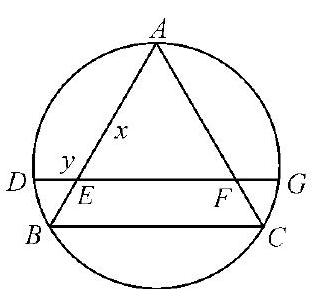
\includegraphics[max width=\textwidth, center]{2024_10_09_7e48ff928cc374c97394g-076}\\
(第26题)

中出现. $\square$\\
28 求所有边长为整数且周长等于面积的两倍 (数值上) 的直角三角形的三边长.\\
29 求边长为整数且面积等于 24 的直角三角形的三边长.\\
30 已知 $\triangle A B C$ 的三边长都是整数, $\angle A=2 \angle B, \angle C>90^{\circ}$. 求 $\triangle A B C$ 的周长的最小值.\\
31 设整数 $a ,  b$ 满足 $5 a \geqslant 7 b \geqslant 0$. 证明: 关于 $x ,  y ,  z, w$ 的方程组\\
\begin{align*}
\left\{\begin{array}{l}
x+2 y+3 z+7 w=a \\
y+2 z+5 w=b
\end{array}\right.
\end{align*}

有非负整数解.\\
32 正整数 $a ,  b ,  c$ 两两互素. 证明: 数 $2 a b c-a b-b c-c a$ 是不能表示为 $x b c+y c a+z a b$ 形式的最大正整数, 这里 $x ,  y ,  z$ 是非负整数.\\
33 设 $n$ 为正整数, 用 $d(n)$ 表示 $n$ 的正因数的个数, $\varphi(n)$ 表示 $1,2, \cdots, n$ 中与 $n$ 互素的数的个数. 求所有的 $n$, 使得 $d(n)+\varphi(n)=n$.\\
34 证明: 存在无穷多个三元正整数数组 $(a, b, c)$, 使得 $a^{2}+b^{2}, b^{2}+c^{2}, c^{2}+$ $a^{2}$ 都是完全平方数.\\
35 证明:不定方程 $x^{2}=y^{5}-4$ 没有整数解. \\
36 证明: 不存在正整数 $m ,  n$, 使得 $19^{19}=m^{3}+n^{4}$.\\
37 是否存在正整数 $x ,  y ,  z ,  u ,  v$, 使得 $x ,  y ,  z ,  u ,  v$ 都大于 2012, 且满足 $x^{2}+y^{2}+z^{2}+u^{2}+v^{2}=x y z u v-65$.\\
38 求所有的整数 $a$, 使得方程 $x^{2}+a x y+y^{2}=1$, 有无穷多组整数解.\\
39 求所有的正整数 $x ,  k ,  n(n \geqslant 2)$, 使得\\
\begin{align*}
3^{k}-1=x^{n}
\end{align*}

40 求使得不定方程\\
\begin{align*}
n=x^{3}-x^{2} y+y^{2}+x-y
\end{align*}

没有正整数解的最小正整数 $n$.

\section{习 题 1}
\begin{enumerate}
  \item 当 $n$ 为偶数时, $n^{4}+4^{n}$ 是大于 2 的偶数, 从而它是合数. 当 $n$ 为奇数时, 设 $n=2 k+1$, 则\\
\begin{align*}
n^{4}+4^{n}=n^{4}+4 \times\left(2^{k}\right)^{4}
\end{align*}
\end{enumerate}

利用\\
\begin{align}
x^{4}+4 y^{4} & =\left(x^{2}+2 y^{2}\right)^{2}-4 x^{2} y^{2} \\
& =\left(x^{2}-2 x y+2 y^{2}\right)\left(x^{2}+2 x y+2 y^{2}\right)
\end{align}

可得出 $n^{4}+4 \times\left(2^{k}\right)^{4}$ 为合数.\\
2. 由 $\left|4 x^{2}-12 x-27\right|=|(2 x+3)(2 x-9)|$, 可知只有 $|2 x+3|=$ 1 或 $|2 x-9|=1$ 时, 数 $\left|4 x^{2}-12 x-27\right|$ 才可能为素数. 依此可得所求的 $x=-2,-1,4$ 或 5 , 对应的 $\left|4 x^{2}-12 x-27\right|$ 分别为 $13,11,11$ 或 13 , 都是素数. \\
3. 若 $m$ 为合数, 则存在正整数 $p$, 使 $2 \leqslant p<m$, 且 $p \mid m$, 此时有 $p \mid(m-$ $1)!$, 但 $m \mid(m-1)!+1$, 故 $p \mid(m-1)!+1$, 这导致 $p \mid 1$, 矛盾.\\
4. 不妨设 $p<q<r$, 则\\
\begin{align*}
q \geqslant p+1, r \geqslant q+2 \geqslant p+3
\end{align*}

对 $d=10$ 的情形,由 $q r \mid p^{2}+10 ,$ 应有\\
\begin{align*}
p^{2}+10 \geqslant(p+1)(p+3)
\end{align*}

这要求 $4 p \leqslant 7$, 即 $p \leqslant 1$, 矛盾. 故 $d=10$ 时不存在符合要求的 $p ,  q ,  r$.\\
当 $d=11$ 时, $p=2, q=3, r=5$ 满足条件.\\
5. 若 $p$ 为合数, 设 $p=q r, 2 \leqslant q \leqslant r$, 则\\
\begin{align*}
2^{p}-1=\left(2^{q}\right)^{r}-1=\left(2^{q}-1\right)\left(\left(2^{q}\right)^{r-1}+\left(2^{q}\right)^{r-2}+\cdots+1\right),
\end{align*}

这导致 $2^{q}-1 \mid 2^{p}-1$ ,与 $2^{p}-1$ 是素数矛盾. 故 $p$ 为素数.\\
6. 由算术基本定理知,可写 $n=2^{k} \cdot q, k \geqslant 0, q$ 为奇数. 若 $q>1$, 则\\
\begin{align}
2^{n}+1 & =\left(2^{2^{k}}\right)^{q}+1 \\
& =(x+1)\left(x^{q-1}-x^{q-2}+\cdots-x+1\right)
\end{align}

是两个大于 1 的正整数之积,不是素数,其中 $x=2^{2^{k}}$ . 依此可知,由 $2^{n}+1$ 为素数可得 $q=1$ ,即命题成立. \\
7. 当 $n=1$ 时, $n^{n}+1=2$ 满足条件. 当 $n>1$ 时, 设 $n=2^{k} q, q$ 为奇数,若 $q>1$ ,同上题可知 $n^{n}+1$ 不是素数,故 $n=2^{k} , k$ 为正整数. 此时\\
\begin{align*}
n^{n}+1=2^{k \cdot 2^{k}}+1=\left(2^{2^{k}}\right)^{k}+1
\end{align*}

进一步的分析,可知存在非负整数 $m$ ,使得 $k=2^{m}$ ,故\\
\begin{align*}
n^{n}+1=2^{2^{2^{m}+m}}+1
\end{align*}

当 $m \geqslant 2$ 时, $2^{m}+m \geqslant 6$, 故 $2^{2^{m}+m} \geqslant 2^{6}$, 因此\\
\begin{align}
n^{n}+1 & \geqslant 2^{2^{6}}+1=2^{64}+1 \\
& =16 \times(1024)^{6}+1 \\
& >16 \times\left(10^{3}\right)^{6}+1 \\
& >10^{19}
\end{align}

故由 $n^{n}+1 \leqslant 10^{19}$ 知 $m \leqslant 1$ . 分别令 $m=0,1$, 知 $n^{n}+1=5,257$, 这两个都是素数. 

综上, 所求的素数为 2,5 和 257 . \\
8. 利用\\
\begin{align}
& (a d+b c)-(a b+c d) \\
= & d(a-c)-b(a-c) \\
= & (d-b)(a-c)
\end{align}

及 $a-c \mid a b+c d ,$ 可得 $a-c \mid a d+b c$ . \\
9. 由恒等式\\
\begin{align*}
(b c+a d)^{2}+(b c-a d)^{2}=4 a b c d=4(a c)(b d)
\end{align*}

结合条件,可知 $u^{2} \mid(b c-a d)^{2}$ ,故 $u \mid b c-a d$ . \\
现在,我们设 $b c+a d=u x, b c-a d=u y$ ,则由(1)知,\\
\begin{align*}
x^{2}+y^{2}=4\left(\frac{a c}{u}\right)\left(\frac{b d}{u}\right)
\end{align*}

故 $x^{2}+y^{2}$ 为偶数,进而 $x+y$ 与 $x-y$ 都是偶数,所以,由\\
\begin{align*}
b c=\frac{x+y}{2} \cdot u, a d=\frac{x-y}{2} \cdot u
\end{align*}

可得 $b c ,  a d$ 都是 $u$ 的倍数. \\
10. 注意到,对任意正整数 $k(\neq b)$ ,都有 $b-k \mid b^{n}-k^{n}$ ,结合 $b-k \mid a-k^{n}$ ,可知 $b-k \mid a-b^{n}$ . 这表明 $a-b^{n}$ 是每个正整数的倍数,故 $a-b^{n}=0$ ,得 $a=b^{n}$ . \\
11. 满足条件的最小的 $n=270$ . 

事实上,由条件知 $10 \mid n$ ,从 $n$ 的末尾数字为 9 的因数出发来讨论. 若 $9 \mid$ $n$ ,则 $90 \mid n$ ,此时直接验证可知 90 和 180 都不是某个末尾为 7 的数的倍数;若 $19 \mid n$ ,则 $190 \mid n$ ,而 $n=190$ 不是某个末尾为 7 的数的倍数. 而 270 分别是 $10,1,2,3,54,5,6,27,18,9$ 的倍数,符合条件. 故 $n$ 最小为 270 . \\
12. 设 $M=\overline{a_{1} a_{2} \cdots a_{9}}$ 是一个满足条件的数,由条件可知 $a_{5}=5$, 并且 $a_{2}$ ,  $a_{4} ,  a_{6} ,  a_{8}$ 是 $2 ,  4 ,  6 ,  8$ 的一个排列,进而, $a_{1} ,  a_{3} ,  a_{7} ,  a_{9}$ 是 $1 ,  3 ,  7 ,  9$ 的排列. 依此可知\\
\begin{align*}
a_{4}=2 \text { 或 } 6\left(\text { 因为 } 4 \mid \overline{a_{3} a_{4}}\right),
\end{align*}

而进一步,还有\\
\begin{align*}
8 \mid \overline{a_{7} a_{8}}
\end{align*}

因此\\
\begin{align*}
a_{8}=2,6
\end{align*}

故\\
\begin{align*}
\left(a_{4}, a_{8}\right)=(2,6),(6,2)
\end{align*}

对这两种情况作进一步的分析,就可找到一个满足条件的 $M=381654729$ . \\
13. 设 $n$ 是一个好数, 则 $n+1=(a+1)(b+1)$ 为一个合数,反过来,若 $n+1$ 为合数,则可写\\
\begin{align*}
n+1=p q, 2 \leqslant p \leqslant q
\end{align*}

于是令 $a=p-1, b=q-1$ ,就有 $n=a b+a+b$ 是一个好数. 所以,只需求 $1,2, \cdots, 100$ 中使 $n+1$ 为合数的 $n$ 的个数, 依此可知恰有 74 个好数.\\
14. 当 $n \geqslant 2$ 时, $p_{n}$ 与 $p_{n+1}$ 都是奇数,于是, $q=\frac{p_{n}+p_{n+1}}{2}$ 是正整数,又 $p_{n}<q<p_{n+1}, p_{n}$ 与 $p_{n+1}$ 是两个相邻的素数,故 $q$ 必为合数. 从而 $q$ 可以写为两个大于 1 的正整数之积,依此可知命题成立. \\
15. 若存在 $a ,  b ,  x ,  y$, 使得\\
\begin{align*}
n=a+b, \text { 且 } \frac{x}{a}+\frac{y}{b}=1 \text {. }
\end{align*}

我们记 $d=(a, b)$ ,若 $d=1$ ,由\\
\begin{align*}
\frac{x}{a}+\frac{y}{b}=1
\end{align*}

知\\
\begin{align*}
b x+a y=a b,
\end{align*}

所以\\
\begin{align*}
a|b x, b| a y
\end{align*}

结合 $(a, b)=1$ ,导出 $a|x, b| y$ ,从而\\
\begin{align*}
a b=b x+a y \geqslant a b+b a=2 a b
\end{align*}

矛盾. 所以 $d>1$, 这时 $n=a+b=d\left(\frac{a}{d}+\frac{b}{d}\right)$ 为合数.\\
反过来, 设 $n$ 为合数, 设 $n=p q, 2 \leqslant p \leqslant q$, 则令 $(a, b, x, y)=$ $(p, p(q-1), 1 ,(p-1)(q-1)) ,$ 就有\\
\begin{align*}
n=a+b, \text { 且 } \frac{x}{a}+\frac{y}{b}=1 \text {. }
\end{align*}\\
16. 注意到 $10001=73 \times 137$ 为合数,而从第二项起, 我们有\\
\begin{align}
a_{n} & =\underbrace{100010001 \cdots 0001}_{n \text { 个0o01 }} \\
& =10^{4 n}+10^{4(n-1)}+\cdots+10^{4}+1 \\
& =\frac{10^{4(n+1)}-1}{10^{4}-1} \\
& =\frac{\left(10^{2(n+1)}-1\right)\left(10^{2(n+1)}+1\right)}{10^{4}-1},
\end{align}

由于 $n \geqslant 2$ 时, $10^{4}-1<10^{2(n+1)}-1<10^{2(n+1)}+1$, 所以, $a_{n}$ 是一个合数.\\
17. 由 $a^{2}-b^{2}+c^{2}-d^{2}=1749$ 为奇数,知 $a ,  b ,  c ,  d$ 中必有一个数为偶数,这表明 $d=2$ . 进而\\
\begin{align*}
a^{2}-b^{2}+c^{2}=1753
\end{align*}

再由\\
\begin{align*}
a>3 b>6 c>12 d
\end{align*}

可知 $c \geqslant 5, b \geqslant 2 c+1, a \geqslant 3 b+1$, 所以\\
\begin{align}
a^{2}-b^{2}+c^{2} & \geqslant(3 b+1)^{2}-b^{2}+c^{2} \\
& =8 b^{2}+6 b+c^{2}+1 \\
& \geqslant 8(2 c+1)^{2}+6(2 c+1)+c^{2}+1 \\
& =33 c^{2}+44 c+15
\end{align}

故\\
\begin{align*}
33 c^{2}+44 c+15 \leqslant 1753
\end{align*}

于是, $c<7$, 结合 $c \geqslant 5$ 及 $c$ 为素数, 可知 $c=5$, 进而\\
\begin{align*}
a^{2}-b^{2}=1728=2^{6} \times 3^{3}
\end{align*}

利用\\
\begin{align*}
b \geqslant 2 c+1=11, a \geqslant 3 b+1
\end{align*}

可知\\
\begin{align*}
a-b \geqslant 2 b+1 \geqslant 23, a+b \geqslant 4 b+1 \geqslant 45
\end{align*}

由 $(a-b)(a+b)=2^{6} \times 3^{3}$ 及 $a ,  b$ 都是奇素数,可知\\
\begin{align*}
(a-b, a+b)=(32,54)
\end{align*}

因此\\
\begin{align*}
(a, b)=(43,11)
\end{align*}\\
\begin{align*}
a^{2}+b^{2}+c^{2}+d^{2}=1749+2 \times\left(11^{2}+2^{2}\right)=1999
\end{align*}\\
18. 对正整数 $n$, 设正整数 $k$ 满足 $\frac{k(k+1)}{2} \leqslant n<\frac{(k+1)(k+2)}{2}$, 则\\
\begin{align}
& a_{1}+a_{2}+\cdots+a_{n} \\
= & 1 \times 1+2 \times 2+\cdots+k \times k+(k+1) \times\left[n-\frac{k(k+1)}{2}\right] \\
= & \frac{1}{6} k(k+1)(2 k+1)+\frac{2 n-k(k+1)}{2}(k+1) \\
= & \frac{1}{6}(k+1)[6 n-k(k+2)] .
\end{align}

由于当 $k \geqslant 6$ 时, $k+1>6$, 有\\
\begin{align*}
6 n-k(k+2) \geqslant 3 k(k+1)-k(k+2)=2 k^{2}+k>6
\end{align*}

所以,此时 $a_{1}+a_{2}+\cdots+a_{n}$ 为合数,即只需考虑 $k \leqslant 5$ 的情形,考察数列\\
\begin{align*}
1,2,2,3,3,3,4,4,4,4,5,5,5,5,5,6,6,6,6,6,6
\end{align*}

从第一项起求和得到的素数分别是:3,5,11,61,67,73,79,共 7 个. 所以仅当 $n=2,3,5,16,17,18,19$ 时, $a_{1}+a_{2}+\cdots+a_{n}$ 为素数. \\
19. 由条件可知, 当 $m \mid n$, 且 $m<n$ 时, 有 $a_{n} \geqslant 2 a_{m}$ . 所以, $a_{1} \geqslant 1, a_{2} \geqslant$ $2, a_{4} \geqslant 2 a_{2} \geqslant 2^{2}$, 类似地, $a_{8} \geqslant 2^{3}, a_{16} \geqslant 2^{4}, a_{80} \geqslant 2^{5}, a_{400} \geqslant 2^{6}, a_{2000} \geqslant 2^{7}$,即 $a_{2000} \geqslant 128$.

另一方面,对任意正整数 $n$ ,设 $n$ 的素因数分解式为\\
\begin{align*}
n=p_{1}^{\alpha_{1}} p_{2}^{\alpha_{2}} \cdots p_{k^{\alpha}}^{\alpha_{k}}
\end{align*}

其中 $p_{1}<p_{2}<\cdots<p_{k}$ 为素数, $\alpha_{1}, \alpha_{2}, \cdots, \alpha_{k}$ 为正整数,定义\\
\begin{align*}
a_{n}=2^{a_{1}+a_{2}+\cdots+\alpha_{k}},
\end{align*}

则数列 $\left\{a_{n}\right\}$ 符合题中的要求,并且\\
\begin{align*}
a_{2000}=2^{4+3} \leqslant 2^{7}
\end{align*}

所以, $a_{2000}$ 的最小值为 128 .\\
20. 由条件,可知\\
\begin{align}
\frac{2 m}{n} & =\left(1+\frac{1}{2}+\cdots+\frac{1}{p-1}\right)+\left(\frac{1}{p-1}+\frac{1}{p-2}+\cdots+1\right) \\
& =\left(1+\frac{1}{p-1}\right)+\left(\frac{1}{2}+\frac{1}{p-2}\right)+\cdots+\left(\frac{1}{p-1}+1\right) \\
& =\frac{p}{1 \times(p-1)}+\frac{p}{2 \times(p-2)}+\cdots+\frac{p}{(p-1) \times 1}
\end{align}

上式将右边通分后,可知存在正整数 $M$ ,使得 $\frac{2 m}{n}=\frac{p M}{(p-1)!}$ ,即 $p n M=$ $2 m(p-1)!$, 由 $p$ 为奇素数, 可知 $p \nmid 2, p \nmid(p-1)!$, 所以, $p \mid m$ . \\
21. 若 $m \nmid n$ ,由 $a^{m}+1 \mid a^{n}+1$ 及 $a>1$ ,可知 $m<n$ . 故可设 $n=m q+$ $r$ ,其中 $q ,  r$ 为正整数, $0<r<m$ . 此时,利用 $a^{m}+1 \mid a^{n}+1$ ,可知\\
\begin{align*}
a^{m}+1 \mid\left(a^{n}+1\right)-\left(a^{m}+1\right)
\end{align*}

即\\
\begin{align*}
a^{m}+1 \mid\left(a^{m-n}+1\right) a^{m},
\end{align*}

而\\
\begin{align*}
\left(a^{m}+1, a^{m}\right)=\left(1, a^{m}\right)=1
\end{align*}

所以\\
\begin{align*}
a^{m}+1 \mid a^{n-m}+1
\end{align*}

依次递推,可得\\
\begin{align*}
a^{m}+1\left|a^{n-2 m}+1, \cdots, a^{m}+1\right| a^{n-m q}+1
\end{align*}

即有\\
\begin{align*}
a^{m}+1 \mid a^{r}+1
\end{align*}

但 $a>1$ 时, $a^{m}+1>a^{r}+1$, 矛盾.\\
所以, $m \mid n$.\\
22. 设 $d=\left(2^{m}-1,2^{n}+1\right)$ ,则\\
\begin{align*}
\begin{gathered}
d \mid 2^{m}-1 \\
d \mid\left(2^{m}\right)^{n}-1^{n} \\
d \mid 2^{m}-1
\end{gathered}
\end{align*}

另外 $d \mid 2^{n}+1$ ,又 $m$ 为奇数,故\\
\begin{align*}
2^{n}+1 \mid\left(2^{n}\right)^{m}+1^{m}
\end{align*}

所以\\
\begin{align*}
d \mid 2^{m n}+1
\end{align*}

对比所得的两个式子,知 $d \mid 2$ ,又 $2^{m}-1$ 为奇数,故 $d=1$ . \\
23. 不妨设 $m<n$ ,利用平方差公式知\\
\begin{align}
F_{n}-2 & =2^{2^{n}}-1 \\
& =\left(2^{2^{n-1}}-1\right)\left(2^{2^{n-1}}+1\right) \\
& =\left(2^{2^{n-2}}-1\right)\left(2^{2^{n-2}}+1\right)\left(2^{2^{n-1}}+1\right) \\
& =\cdots \\
& =\left(2^{2^{m}}-1\right)\left(2^{2^{m}}+1\right)\left(2^{2^{m+1}}+1\right) \cdots\left(2^{2^{n-1}}+1\right)
\end{align}

所以, $F_{m} \mid F_{n}-2$ ,从而 $\left(F_{n}, F_{m}\right)=\left(2, F_{m}\right)$ ,而 $F_{m}$ 为奇数,故 $\left(2, F_{m}\right)=1$ ,即 $\left(F_{n}, F_{m}\right)=1$ . \\
24. 由条件可知 $a ,  b ,  c ,  d$ 不全相等, 不妨设 $d$ 是其中最大的数,则\\
\begin{align*}
d<a+b+c+d<4 d
\end{align*}

又 $a+b+c+d$ 为 $a ,  b ,  c ,  d$ 的最小公倍数,故

于是\\
\begin{align*}
\begin{gathered}
d \mid a+b+c+d, \\
a+b+c+d=2 d \text { 或 } 3 d .
\end{gathered}
\end{align*}

如果 $a+b+c+d=3 d$ ,那么由 $a b c d$ 为 $a ,  b ,  c ,  d$ 的公倍数,可知\\
\begin{align*}
a+b+c+d \mid a b c d
\end{align*}

即\\
\begin{align*}
3 d \mid a b c d
\end{align*}

故\\
\begin{align*}
3 \mid a b c d
\end{align*}

如果 $a+b+c+d=2 d$ ,那么 $a+b+c=d$ . 不妨设 $a \leqslant b \leqslant c$ ,由 $a+$ $b+c+d$ 为 $a ,  b ,  c ,  d$ 的最小公倍数,可知\\
\begin{align*}
a|2 d, b| 2 d, c \mid 2 d
\end{align*}

设 $2 d=a x=b y=c z$ ,则 $x \geqslant y \geqslant z \geqslant 3$ ,并且\\
\begin{align*}
\frac{2}{x}+\frac{2}{y}+\frac{2}{z}=1
\end{align*}

即\\
\begin{align*}
\frac{1}{x}+\frac{1}{y}+\frac{1}{z}=\frac{1}{2}
\end{align*}

又当 $z=3$ 时,有 $3 \mid 2 d$ ,进而 $3 \mid d$ ,故 $a b c d$ 为 3 的倍数,因此只需考虑 $z>3$ 的情形. 

而当 $z \geqslant 6$ 时, 有\\
\begin{align*}
\frac{1}{x}+\frac{1}{y}+\frac{1}{z} \leqslant \frac{1}{6}+\frac{1}{6}+\frac{1}{6}=\frac{1}{2}
\end{align*}

故只能是 $x=y=z=6$, 此时 $a b c d$ 为 3 的倍数.\\
所以, 只需考虑 $z=4$ 或 5 的情形, 注意到 $z=5$ 时, 有 $5 \mid 2 d$, 可知 $a b c d$是 5 的倍数, 进而只需考虑 $z=4$ 的情形, 此时\\
\begin{align*}
\frac{1}{x}+\frac{1}{y}=\frac{1}{4}
\end{align*}

即\\
\begin{align*}
x y-4 x-4 y=0
\end{align*}\\
\begin{align*}
(x-4)(y-4)=16
\end{align*}

结合 $x>y$, 可知\\
\begin{align*}
(x-4, y-4)=(16,1),(8,2),(4,4)
\end{align*}

分别对应\\
\begin{align}
& 2 d=20 a=5 b=4 c, \\
& 2 d=12 a=6 b=4 c \\
& 2 d=8 a=8 b=4 c
\end{align}

第一种情形要求 $5 \mid d$ ,第二种情形要求 $3 \mid d$ ,第三种情形要求\\
\begin{align*}
a=b, c=2 a, d=4 a,
\end{align*}

此时 $a ,  b ,  c ,  d$ 的最小公倍数为 $d$, 而不是 $a+b+c+d$, 矛盾.\\
综上可知, $a b c d$ 是 3 或 5 的倍数.\\
25. 如果 $n$ 至少有两个不同的素因子, 那么可记 $n=p q$, 其中 $2 \leqslant p<q$, $p ,  q$ 为正整数, 且 $(p, q)=1$. 此时, $2 \leqslant p<q<n-1$, 从而 $n \mid M_{n-1}$, 因此 $M_{n}=M_{n-1}$ . 

如果 $n=p^{\alpha}, p$ 为素数, $\alpha$ 为正整数, 那么 $1,2, \cdots, n-1$ 中每一个数含 $p$的幂次小于 $\alpha$, 此时 $M_{n}=p M_{n-1}$ . 

所以, 当且仅当 $n$ 有至少两个不同的素因子时, $M_{n}=M_{n-1}$.\\
26. 不妨设 $m>n$, 则\\
\begin{align}
\left(a^{m}-1, a^{n}-1\right) & =\left(a^{m}-a^{n}, a^{n}-1\right) \\
& =\left(a^{n}\left(a^{m-n}-1\right), a^{n}-1\right),
\end{align}

而\\
\begin{align*}
\left(a^{n}, a^{n}-1\right)=1,
\end{align*}

故\\
\begin{align*}
\left(a^{m}-1, a^{n}-1\right)=\left(a^{m-n}-1, a^{n}-1\right)
\end{align*}

依次递推,对指数进行"辗转相除",可知结论成立. \\
27. 由 $a^{n}+1$ 为素数,可知 $a$ 为偶数,与第 6 题类似,可知存在非负整数 $k$ ,使得 $n=2^{k}$ ,于是\\
\begin{align}
& a^{n}-1 \\
= & a^{2^{k}}-1 \\
= & \left(a^{2^{k-1}}-1\right)\left(a^{2^{k-1}}+1\right) \\
= & \cdots \\
= & (a-1)(a+1)\left(a^{2}+1\right) \cdots\left(a^{2^{k-1}}+1\right)
\end{align}

进一步, $\left(a^{2^{k-1}}-1, a^{2^{k-1}}+1\right)=\left(a^{2^{k-1}}-1,2\right)=1$ (最后一步用到 $a$ 为偶数),依次倒推,可知 $a+1, a^{2}+1 , a^{2^{2}}+1 , \cdots , a^{2^{k-1}}+1$ 两两互素,从而它们中任取若干个数作乘积形成的 $2^{k}$ 个数两两不同,当然,这 $2^{k}$ 个数都是 $a^{n}-1$的因数,所以, $d\left(a^{n}-1\right) \geqslant 2^{k}=n$ . \\
28. 当 $n=3$ 时,对任意三个连续正整数 $a-1, a, a+1$, 若

则\\
而\\
故\\
\begin{align}
& a+1 \mid[a-1, a] \\
& a+1 \mid a(a-1) \\
& (a+1, a)=1 \\
& a+1 \mid a-1
\end{align}

矛盾. \\
当 $n>3$ 时,若 $n$ 为偶数,记 $n=2 m$ ,则数 $2 m-1,2 m, \cdots, 2(2 m-1)$中,最大的数 $2(2 m-1)$ 是其余 $2 m-1$ 个数(它们中有 $2 m-1$ 与 $2 m$ )的最小公倍数的因数;若 $n$ 为奇数,记 $n=2 m+1$ ,则数 $2 m-2 , 2 m-1 , \cdots$ , $2(2 m-1)$ 是 $n$ 个连续正整数(注意,这里用到 $m>1$ ),它们中最大的数是其余 $n-1$ 个数的最小公倍数的因数. 

所以, $n>3$ 时,正整数 $n$ 符合条件.\\
29. 利用\\
\begin{align*}
a^{n}+b^{n}=\left(a^{n-m}+b^{n-m}\right)\left(a^{m}+b^{m}\right)-\left(a^{m} b^{n-m}+a^{n-m} b^{m}\right)
\end{align*}

知若 $n \geqslant 2 m$ ,则\\
\begin{align*}
a^{n}+b^{n}=\left(a^{n-m}+b^{n-m}\right)\left(a^{m}+b^{m}\right)-a^{m} b^{m}\left(a^{n-2 m}+b^{n-2 m}\right),
\end{align*}

于是\\
\begin{align*}
a^{m}+b^{m} \mid a^{m} b^{m}\left(a^{n-2 m}+b^{n-2 m}\right)
\end{align*}

由\\
\begin{align*}
(a, b)=1
\end{align*}

得\\
\begin{align*}
\left(a^{m}, b^{m}\right)=1
\end{align*}

进而\\
\begin{align*}
\left(a^{m}+b^{m}, a^{m}\right)=\left(a^{m}+b^{m}, b^{m}\right)=1
\end{align*}

故\\
\begin{align*}
\left(a^{m}+b^{m}, a^{m} b^{m}\right)=1
\end{align*}

因此\\
\begin{align*}
a^{m}+b^{m} \mid a^{n-2 m}+b^{n-2 m}
\end{align*}

用 $n-2 m$ 代替 $n$ ,重复上述讨论,最终可将 $n$ 变为小于 $2 m$ 的正整数. 此时,由 $a^{m}+b^{m} \mid a^{n}+b^{n}$ 及 $a>1$ ,知 $n \geqslant m$ . 如果 $n=m$ ,那么命题已经成立;如果 $m<n<2 m$ ,那么由\\
\begin{align*}
a^{n}+b^{n}=\left(a^{n-m}+b^{n-m}\right)\left(a^{m}+b^{m}\right)-a^{n-m} b^{n-m}\left(a^{2 m-n}+b^{2 m-n}\right),
\end{align*}

同上讨论,将有\\
\begin{align*}
a^{m}+b^{m} \mid a^{2 m-n}+b^{2 m-n}
\end{align*}

而 $2 m-n<m$ ,这在 $a>1$ 时是不可能的. \\
综上可知 $m \mid n$ (注意:事实上推出了 $n$ 为 $m$ 的奇数倍).\\
30. 将命题一般化,可证:对任意 $n(\geqslant 2)$ ,都存在 $n$ 个不同的正整数,使得其中任意两个不同的数 $a, b$ 满足 $(a-b)^{2} \mid a b$ . 证明如下:

当 $n=2$ 时,取 $a_{1}=1, a_{2}=2$ ,则它们满足条件. \\
现在设 $a_{1}<a_{2}<\cdots<a_{n}$ 是 $n(\geqslant 2)$ 个满足要求的正整数,即对 $1 \leqslant i<$ $j \leqslant n$ ,都有 $\left(a_{i}-a_{j}\right)^{2} \mid a_{i} a_{j}$ . 

考虑下面的 $n+1$ 个数\\
\begin{align*}
a_{n}!, a_{n}!+a_{1}, a_{n}!+a_{2}, \cdots, a_{n}!+a_{n}
\end{align*}

容易证明这 $n+1$ 个正整数满足要求. \\
31. 对任意正整数 $m$ ,由 $(a, b)=1$ ,可写 $m=m_{1} m_{2}$ ,使得 $m_{1}$ 的素因子都是 $a$ 的素因子,且\\
\begin{align*}
\left(a, m_{2}\right)=1,\left(m_{1}, b\right)=1,\left(m_{1}, m_{2}\right)=1
\end{align*}\\
(这只需将 $m ,  a ,  b$ 作素因数分解后,各部分予以恰当分配即可达到要求).\\
取正整数 $k$, 使得 $\left(k, m_{1}\right)=1$ ,这样的 $k$ 有无穷多个,令 $n=m_{2} k$ ,我们证明: $\left(a+n b, m_{1}\right)=1$ . 

事实上, 设 $d=\left(a+n b, m_{1}\right)$, 若 $d>1$, 取 $d$ 的素因子 $p$, 则 $p \mid m_{1}$, 进而 $p \mid a$ ,所以, $p \mid n b$ . 

但由 $\quad\left(m_{1}, k\right)=\left(m_{1}, m_{2}\right)=\left(m_{1}, b\right)=1$,\\
知 $p \nmid m_{2} k b$ ,即 $p \nmid n b$ . 矛盾. 所以\\
\begin{align*}
\left(a+n b, m_{1}\right)=1
\end{align*}

又 $\left(a+n b, m_{2}\right)=\left(a+m_{2} k b, m_{2}\right)=\left(a, m_{2}\right)=1$ ,\\
从而\\
\begin{align*}
\left(a+n b, m_{1} m_{2}\right)=1
\end{align*}

即\\
\begin{align*}
(a+n b, m)=1
\end{align*}

命题获证.\\
32. 设 $a ,  b$ 的素因数分解式中 $2 ,  5$ 的幂次分别为 $\alpha_{1} ,  \beta_{1}$ 和 $\alpha_{2} ,  \beta_{2}$, 则\\
\begin{align*}
\left\{\begin{array}{l}
a \cdot \alpha_{1}+b \cdot \alpha_{2} \geqslant 98 \\
a \cdot \beta_{1}+b \cdot \beta_{2} \geqslant 98
\end{array}\right.
\end{align*}

并且(1)与(2)中必有一个取等号.\\
如果(2)取等号,即 $a \cdot \beta_{1}+b \cdot \beta_{2}=98$ ,那么当 $\beta_{1}$ 与 $\beta_{2}$ 都是正整数时,左边为 5 的倍数,当 $\beta_{1}$ 或 $\beta_{2}$ 中有一个为零时,另一个必大于零,此时左边仍然是 5 的倍数,都导致矛盾. 所以(1)取等号. 

由 $a \cdot \alpha_{1}+b \cdot \alpha_{2}=98$ ,知若 $\alpha_{1} ,  \alpha_{2}$ 中有一个为零,不妨设 $\alpha_{2}=0$ ,则 $\alpha_{1}>$ 0 . 此时 $a \cdot \alpha_{1}=98$ ,若 $\alpha_{1} \geqslant 2$ ,则 $4 \mid a$ ,矛盾. 故 $\alpha_{1}=1$ ,进而 $a=98$ . 代入 (2),由 $a=98$ 知 $\beta_{1}=0$ ,从而 $b \cdot \beta_{2}>98$ ,结合 $\alpha_{2}=0$ ,求得 $b$ 最小为 75 . 

如果 $\alpha_{1}$ 与 $\alpha_{2}$ 都是正整数,不妨设 $\alpha_{1} \geqslant \alpha_{2}$ ,若 $\alpha_{2} \geqslant 2$ ,则有 $4|a , 4| b$ ,导致 $4 \mid 98$ ,矛盾,故 $\alpha_{2}=1$ . 进一步,若 $\alpha_{1}=1$ ,则 $a+b=98$ ,但 $\frac{a}{2}$ 与 $\frac{b}{2}$ 都是奇数,故 $\frac{a}{2}+\frac{b}{2}$ 为偶数,矛盾,故 $\alpha_{1}>1$ . 此时,若 $\beta_{1}$ 与 $\beta_{2}$ 都是正整数,则 $5 \mid a$ , $5 \mid b$ ,与 $a \cdot \alpha_{1}+b \cdot \alpha_{2}=98$ 矛盾,故 $\beta_{1}$ 与 $\beta_{2}$ 中有一个为零. 若 $\beta_{1}=0$ ,则由(2)知 $b \beta_{2}>98$ ,此时 $b^{b}$ 的末尾零的个数大于 98 (因为,此时 $10 \mid b$ . 当 $\beta_{2}=1$ 时, $b \geqslant 100$ ,此时 $10^{100} \mid b^{b}$ . 而当 $\beta_{2} \geqslant 2$ 时,50| $b$ ,若 $b>50$ ,则 $10^{100} \mid b^{b}$ ;若 $b=50$ ,则 $a \cdot \alpha_{1}=48$ ,这时当 $\alpha_{1} \geqslant 4$ 时, $2^{5} \mid a \cdot \alpha_{1}$ ,而 $\alpha_{1} \leqslant 3$ 时, $2^{4} \nmid a \cdot \alpha_{1}$都导致矛盾,所以, $b^{b}$ 的末尾零的个数大于 98). 

类似地,若 $\beta_{2}=0$ ,则 $a \cdot \beta_{1}>98$ ,同样可知 $a^{a}$ 的末尾零的个数大于 98 ,矛盾. 综上可知, $a b$ 的最小值为 7350 (当 $(a, b)=(98,75)$ 或 $(75,98)$ 时取到). \\
33. 由条件可知 $m$ 为一个 4 次方数, 因此, 可设\\
\begin{align*}
m=2^{4 \alpha_{2}} \cdot 3^{4 \alpha_{3}} \cdot 5^{4 \alpha_{5}} \cdot 7^{4 \alpha_{7}} \cdots
\end{align*}

其中 $\alpha_{2}, \alpha_{3}, \alpha_{5}, \alpha_{7}, \cdots$ 都是非负整数.而\\
\begin{align*}
d(m)=\left(4 \alpha_{2}+1\right)\left(4 \alpha_{3}+1\right) \cdots
\end{align*}

是一个奇数,故 $\alpha_{2}=0$, 并且\\
\begin{align*}
1=\frac{4 \alpha_{3}+1}{3^{\alpha_{3}}} \cdot \frac{4 \alpha_{5}+1}{5^{\alpha_{5}}} \cdot \frac{4 \alpha_{7}+1}{7^{\alpha_{7}}} \cdots=x_{3} x_{5} x_{7} \cdots
\end{align*}

这里\\
\begin{align*}
x_{3}=\frac{4 \alpha_{3}+1}{3^{\alpha_{3}}}, x_{5}=\frac{4 \alpha_{5}+1}{5^{\alpha_{5}}}, \cdots
\end{align*}

当 $\alpha_{3}=1$ 时,$x_{3}=\frac{5}{3} ; \alpha_{3}=0$ 或 2 时, $x_{3}=1$ ;而 $\alpha_{3} \geqslant 3$ 时, $3^{\alpha_{3}}>$ $4 \alpha_{3}+1$, 故此时 $x_{3}<1$.

当 $\alpha_{5}=0$ 或 1 时, $x_{5}=1 ; \alpha_{5} \geqslant 2$ 时, $5^{\alpha_{5}} \geqslant 12 \alpha_{5}+1$ ,故 $5^{\alpha_{5}} \geqslant \frac{25}{9}\left(4 \alpha_{5}+\right.$ 1),即 $x_{5} \leqslant \frac{9}{25}$.

当 $p>5, p$ 为素数时,在 $\alpha_{p}=0$ 时, $x_{p}=1$ ,而 $\alpha_{p}=1$ 时, $p^{\alpha} p_{p}>5=$ $4 \alpha_{p}+1$ ,故 $x_{p}<1$ ;而 $\alpha_{p}>1$ 时, $x_{p}<\frac{9}{25}$ . 

上述讨论表明: 若 $\alpha_{3} \neq 1$ ,则

故\\
\begin{align*}
x_{3}=x_{5}=x_{7}=\cdots=1
\end{align*}

而\\
\begin{align*}
\alpha_{3}=0 \text { 或 } 2, \alpha_{5}=0 \text { 或 } 1,
\end{align*}\\
\begin{align*}
\alpha_{7}=\alpha_{11}=\cdots=0
\end{align*}

即\\
\begin{align*}
m=1,3^{8}, 5^{4} \text { 或 } 45^{4} .
\end{align*}

若 $\alpha_{3}=1$ ,则 $3 \mid m$ ,此时,由 $m=d(m)^{4}$ ,知\\
\begin{align*}
m=5^{4} \times\left(4 \alpha_{5}+1\right)^{4} \times\left(4 \alpha_{7}+1\right)^{4} \cdots
\end{align*}

于是存在素数 $p \geqslant 5$, 使得 $3 \mid 4 \alpha_{p}+1$, 这要求 $\alpha_{p} \geqslant 2$, 从而 $x_{p}<\frac{9}{25}$. 此导致\\
\begin{align*}
x_{3} x_{5} x_{7} \cdots \leqslant \frac{5}{3} \times \frac{9}{25}=\frac{3}{5}<1
\end{align*}

矛盾.\\
所以\\
\begin{align*}
m=1,5^{4}, 3^{8}, 3^{8} \cdot 5^{4}
\end{align*}\\
(直接验证,可知它们确实满足条件). \\
34. 设 $n$ 为正整数,如果 $n$ 为偶数,那么表示 $n=(2 n)-n$ 符合要求. 如果 $n$ 为奇数,设 $p$ 是不整除 $n$ 的最小奇素数,那么表示 $n=p n-(p-1) n$ 中, $p n$的素因子个数等于 $n$ 的素因子个数加上 1 ;而 $p-1$ 是偶数,且由 $p$ 的定义,知 $p-1$ 的每个奇素因子都是 $n$ 的素因子,所以, $(p-1) n$ 的素因子个数也等于 $n$ 的素因子个数加上 1 . 命题获证. \\
35. 不妨设 $a \leqslant b$ ,由条件知\\
\begin{align*}
a^{2}\left(b^{2}+1\right)=c^{2}+1-b^{2}-1=(c-b)(c+b)
\end{align*}

故 $b^{2}+1 \mid c-b$ 或者 $b^{2}+1 \mid c+b$ (这里用到 $b^{2}+1$ 为素数). \\
若\\
\begin{align*}
b^{2}+1 \mid c-b
\end{align*}

则\\
\begin{align*}
c-b \geqslant b^{2}+1 \text { (注意 } c>b \text { 是显然的), }
\end{align*}

即\\
\begin{align*}
c \geqslant b^{2}+b+1
\end{align*}

此时\\
\begin{align*}
c^{2}+1 \geqslant\left(b^{2}+b+1\right)^{2}+1>\left(b^{2}+1\right)^{2} \geqslant\left(a^{2}+1\right)\left(b^{2}+1\right)
\end{align*}

矛盾.\\
若\\
\begin{align*}
b^{2}+1 \mid c+b
\end{align*}

则\\
\begin{align*}
c+b \geqslant b^{2}+1
\end{align*}

即\\
\begin{align*}
c \geqslant b^{2}-b+1
\end{align*}

于是\\
\begin{align}
c^{2}+1 & \geqslant\left(b^{2}-b+1\right)^{2}+1 \\
& =\left(b^{2}+1\right)^{2}-2 b\left(b^{2}+1\right)+b^{2}+1 \\
& =\left(b^{2}+1\right)\left((b-1)^{2}+1\right)
\end{align}

注意到,若 $a=b$ ,则 $c^{2}+1=\left(a^{2}+1\right)^{2}$ ,这在 $a ,  c$ 都是正整数时不能成立(因为两个正整数的平方差至少为 3 ),所以, $a<b$ ,即有 $a \leqslant b-1$ ,因此\\
\begin{align*}
c^{2}+1 \geqslant\left(b^{2}+1\right)\left((b-1)^{2}+1\right) \geqslant\left(b^{2}+1\right)\left(a^{2}+1\right)
\end{align*}

结合条件, 可知\\
\begin{align*}
a=b-1, c=b^{2}-b+1
\end{align*}

此时,由 $a^{2}+1$ 与 $b^{2}+1$ 都是素数,知 $b^{2}+1$ 为奇数, $b$ 为偶数,从而 $a=b-1$为奇数, $a^{2}+1$ 为偶数,所以 $a=1$ ,进而 $b=2 , c=3$ . 又当 $(a, b, c)=$ $(1,2,3)$ 或 $(2,1,3)$ 时, 条件满足, 它们就是要求的答案.\\
36. 记 $S_{n}=\sum_{k=1}^{n} \frac{p(k)}{k}$ ,则由 $p(k)$ 的定义可知\\
\begin{align}
S_{2 n} & =\sum_{k=1}^{2 n} \frac{p(k)}{k}=\sum_{k=1}^{n} \frac{p(2 k-1)}{2 k-1}+\sum_{k=1}^{n} \frac{p(2 k)}{2 k} \\
& =n+\frac{1}{2} \sum_{k=1}^{n} \frac{p(2 k)}{k}=n+\frac{1}{2} S_{n}
\end{align}

类似可知\\
\begin{align*}
S_{2 n+1}=n+1+\frac{1}{2} S_{n}
\end{align*}

回到原题, 当 $n=1$ 时, 命题显然成立. 现设命题对 $1 \leqslant n \leqslant m$ 都成立, 考虑 $n=m+1$ 的情形.

如果 $m+1$ 为偶数, 那么, 由(1)结合归纳假设, 可知\\
\begin{align}
& \quad \frac{m+1}{2}+\frac{1}{2} \cdot \frac{2\left(\frac{m+1}{2}\right)}{3}<\frac{m+1}{2}+\frac{1}{2} S_{\frac{w+1}{2}}=S_{m+1}<\frac{m+1}{2}+\frac{1}{2} \\
& \frac{2\left(\frac{m+1}{2}+1\right)}{3}
\end{align}

即有 $\frac{2}{3}(m+1)<S_{m+1}<\frac{2}{3}(m+2)$ ,知命题对 $m+1$ 亦成立.\\
如果 $m+1$ 为奇数, 同上利用(2)亦可知命题对 $m+1$ 成立.\\
所以, 结论成立.\\
37. 由对称性, 不妨设 $a \geqslant b \geqslant c$, 注意到, 当 $(a, b, c)=(2,2,2),(3$, $2,2),(3,3,2),(4,2,2)$ 时, 所给代数式 $A$ 的值分别为 $2, \frac{3}{2}, \frac{17}{8}, \frac{11}{4}$. 这表明: 当 $a+b+c \leqslant 8$ 时, $A \geqslant \frac{3}{2}$.

下证: 当 $a+b+c \geqslant 9$ 时, 有 $A \geqslant \frac{3}{2}$.

\section{事实上,}
\begin{align}
A \geqslant \frac{3}{2} & \Leftrightarrow(a+b+c)^{2}-2([a, b]+[b, c]+[c, a]) \geqslant 3(a+b+c) \\
& \Leftrightarrow a^{2}+b^{2}+c^{2}+2 \sum(a b-[a, b]) \geqslant 3(a+b+c) .
\end{align}

由于对正整数 $x ,  y$, 都有 $x y \geqslant[x, y]$, 因此, 只要证明:\\
\begin{align*}
a^{2}+b^{2}+c^{2} \geqslant 3(a+b+c)
\end{align*}

结合 $a+b+c \geqslant 9$, 可知为证明(1)成立, 只要证明:\\
\begin{align}
& a^{2}+b^{2}+c^{2} \geqslant \frac{1}{3}(a+b+c)^{2} \\
\Leftrightarrow & 3\left(a^{2}+b^{2}+c^{2}\right) \geqslant(a+b+c)^{2} \\
\Leftrightarrow & 2\left(a^{2}+b^{2}+c^{2}\right)-2(a b+b c+c a) \geqslant 0 \\
\Leftrightarrow & (a-b)^{2}+(b-c)^{2}+(c-a)^{2} \geqslant 0 .
\end{align}

最后一式显然成立.\\
所以, 所求代数式的最小值为 $\frac{3}{2}$.\\
38. 记 $u=(a, c), v=(b, c)$ ,则条件 (2) 变为\\
\begin{align*}
\frac{\frac{a c}{u}+\frac{b c}{v}}{a+b}=\frac{p^{2}+1}{p^{2}+2} \cdot c
\end{align*}

即\\
\begin{align*}
\frac{a}{u}+\frac{b}{v}=\frac{p^{2}+1}{p^{2}+2}(a+b)
\end{align*}

由于 $\frac{1}{2}<1-\frac{1}{p^{2}+2}=\frac{p^{2}+1}{p^{2}+2}<1$ ,结合(1)知\\
\begin{align*}
\frac{a+b}{2}<\frac{a}{u}+\frac{b}{v}<a+b
\end{align*}

若 $u ,  v$ 都不小于 2,则(2)的左边不等式不成立;若 $u=v=1$ ,则(2)的右边不等式不成立. 因此 $u, v$ 中恰有一个等于 1 . 

由对称性,不妨设 $u=1, v \geqslant 2$ . 并记 $b_{1}=\frac{b}{v}$ ,代入 (1) 得 $\left(p^{2}+2\right)\left(a+b_{1}\right)=$ $\left(p^{2}+1\right)\left(a+b_{1} v\right)$ ,于是,\\
\begin{align*}
a=b_{1}\left(\left(p^{2}+1\right) v-\left(p^{2}+2\right)\right) .
\end{align*}

若 $v \geqslant 3$ ,则由 (3) 得 $a \geqslant 3\left(p^{2}+1\right)-\left(p^{2}+2\right)=2 p^{2}+1$ ,与条件(1)不符,故 $v=2$ . 此时 (3) 式变为 $a=p^{2} b_{1}$ ,结合 $a \leqslant 2 p^{2}$ ,知 $b_{1} \leqslant 2$ . 

注意到, $(a, c)=u=1,(b, c)=v=2$ ,知 $c$ 是一个偶数,且与 $p^{2} b_{1}$ 互素. 这表明 $p$ 为奇素数, 且 $b_{1}$ 为奇数, 结合 $b_{1} \leqslant 2$ ,知 $b_{1}=1$ ,进而 $b=2$ . 所以, $(a, b, c)=\left(p^{2}, 2, c\right)$ ,其中 $c$ 为偶数但不是 $p$ 的倍数,这样的数组共有 $p^{2}-p$ 组. 

综上可知,当 $p=2$ 时,不存在符合条件的数组;当 $p>2$ 时,满足条件的数组共有 $p^{2}-p$ 组. \\
39. 考虑目标函数 $S=$ 黑板上所有数之积.

最初 $S=33!=2^{31} \cdot 3^{15} \cdot 5^{7} \cdot 7^{4} \cdot 11^{3} \cdot 13^{2} \cdot 17 \cdot 19 \cdot 23 \cdot 29 \cdot 31$ ,每一步操作针对 $x ,  y(x \mid y)$ ,记 $y=k x$ ,去掉 $x ,  y$ 代之以 $k$ 后, $S$ 变为 $\frac{S}{x y} \cdot k=\frac{S}{x^{2}}$ ,这表明每次操作, $S$ 的每个素因子的幂次的奇偶性保持不变,特别地,2,3,5, 11 都整除每次操作后所得的 $S$ . 而 $2 \times 3 \times 5 \times 11>33$ ,因而,最后留下的数中,至少需要两个数,使得它们之积为 $2 \times 3 \times 5 \times 11$ 的倍数. 

又注意到,素数 $17 , 19 , 23 , 29 , 31$ 的每一个大于自身的倍数都大于 33 ,因而,任何一次操作都不能去掉其中的任何一个数. 

上述讨论表明:黑板上至少剩下 7 个数. \\
下面的例子表明可以恰好剩下 7 个数:\\
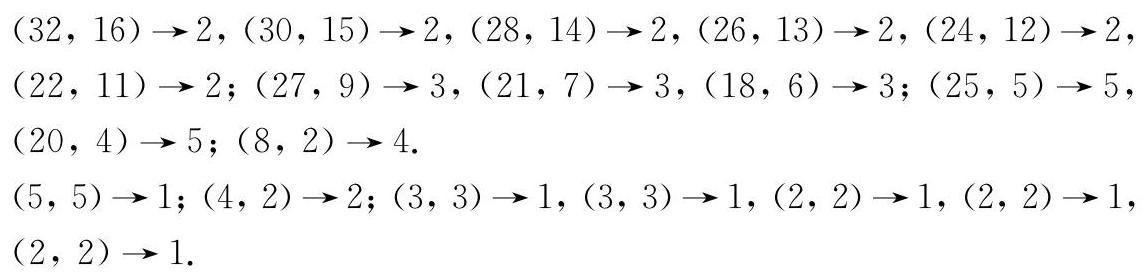
\includegraphics[max width=\textwidth, center]{2024_10_09_7e48ff928cc374c97394g-093}

这样,黑板上留下 $10 , 17 , 19 , 23 , 29 , 31 , 33$ 共 7 个数和 7 个 1 ,而 7 个 1 再经与 17 搭配操作 7 次即可全部去掉. 

综上可知,至少有 7 个数被留下. \\
40. 当 $n$ 为偶数时,设 $n=2 m, x=5^{m}$ ,则\\
\begin{align}
A & =1+5^{n}+5^{2 n}+5^{3 n}+5^{4 n}=1+x^{2}+x^{4}+x^{6}+x^{8} \\
& =\frac{x^{10}-1}{x^{2}-1}=\frac{\left(x^{5}-1\right)\left(x^{5}+1\right)}{(x-1)(x+1)} \\
& =\left(x^{4}+x^{3}+x^{2}+x+1\right)\left(x^{4}-x^{3}+x^{2}-x+1\right) .
\end{align}

由于 $x=5^{m}>1$ ,可知上式右边两个式子中的数都大于 1 ,因此, $A$ 为合数. \\
当 $n$ 为奇数时, 设 $n=2 m+1, y=5^{m}, z=5 y^{2}$ ,则\\
\begin{align}
A & =1+z+z^{2}+z^{3}+z^{4} \\
& =\left(1+3 z+z^{2}\right)^{2}-5 z^{3}-10 z^{2}-5 z \\
& =\left(1+3 z+z^{2}\right)^{2}-5 z(z+1)^{2} \\
& =\left(1+5 y^{2}+25 y^{4}\right)^{2}-25 y^{2}\left(1+5 y^{2}\right)^{2} \\
& =\left(1+5 y^{2}+25 y^{4}-5 y\left(1+5 y^{2}\right)\right)\left(1+5 y^{2}+25 y^{4}+5 y\left(1+5 y^{2}\right)\right)
\end{align}

当 $m>0$, 即 $y \geqslant 5$ 时, 上式右边两式都大于 1 ,此时, $A$ 为合数,当 $m=0$ 时, $A=1+5+5^{2}+5^{3}+5^{4}=781=11 \times 71$ 也是合数. 

所以,对任意正整数 $n, A$ 为合数,命题获证. 

\section{习 题 2}
\begin{enumerate}
  \item 若 $p ,  q$ 都是奇数,则 $7 p+q$ 为偶数, 它不是素数, 故 $p ,  q$ 中有一个为偶数. 
\end{enumerate}

情形一 设 $p$ 为偶数,则 $p=2$ ,此时由 $7 p+q$ 为素数,知 $q$ 为奇素数,若 $q \neq 3$ ,则 $q \equiv 1$ 或 $2(\bmod 3)$ . 

若 $q \equiv 1(\bmod 3) ,$ 则\\
\begin{align*}
7 p+q=14+q \equiv 0(\bmod 3)
\end{align*}

矛盾;

若 $q \equiv 2(\bmod 3) ,$ 则\\
\begin{align*}
p q+11=2 q+11 \equiv 4+11 \equiv 0(\bmod 3)
\end{align*}

亦矛盾, 所以 $q=3$, 此时\\
\begin{align*}
7 p+q=17, p q+11=17
\end{align*}

都是素数,故\\
\begin{align*}
\left(p^{2}+q^{p}\right)\left(q^{2}+p^{q}\right)=\left(2^{2}+3^{2}\right)\left(3^{2}+2^{3}\right)=221
\end{align*}

情形二 设 $q$ 为偶数,则 $q=2$ . 同上讨论可知 $p=3$ ,此时\\
\begin{align*}
\left(p^{2}+q^{p}\right)\left(q^{2}+p^{q}\right)=\left(3^{2}+2^{3}\right)\left(2^{2}+3^{2}\right)=221
\end{align*}

综上可知,所求的值为 221 .\\
2. 设 $d$ 为公差,则 $p_{1}, p_{1}+d, p_{1}+2 d, p_{1}+3 d, p_{1}+4 d$ 都是素数. 

若 $2 \nmid d$ ,即 $d$ 为奇数,则 $p_{1}+d$ 与 $p_{1}+2 d$ 中有一个为偶数,它不是素数. \\
若 $3 \nmid d$ ,则 $p_{1}+d , p_{1}+2 d , p_{1}+3 d$ 中有一个为 3 的倍数(它们构成模 3 的一个完系),矛盾. 

若 $5 \nmid d$ ,则 $p_{1}, p_{1}+d, \cdots, p_{1}+4 d$ 中有一个是 5 的倍数,只能是 $p_{1}=$ 5 ,这时公差 $d$ 是 6 的倍数. 

而 $5,11,17,23,29$ 是 5 个成等差的素数数列,所以, $p_{5}$ 最小为 29 . \\
3. 注意到, 对任意正整数 $k, S(1 \underbrace{0 \cdots 08}_{k \uparrow})=9$ ,于是,设 $1 \underbrace{0 \cdots 08}_{k \uparrow}=3 n$ ,则\\
\begin{align*}
n=\underbrace{3 \cdots 36}_{k \uparrow},
\end{align*}

故 $S(n)=3 k+6$. 这样,对任意正整数 $m$ ,取 $k=3 m-2$ ,就有\\
\begin{align*}
S(n)=m S(3 n)
\end{align*}

说明 由 $S(3 n) \equiv 3 n(\bmod 9)$ ,故要求 $3 \mid S(n)$ ,进而 $3 \mid n$ ,所以在先确定 $3 n$ 时,要寻找一个 9 的倍数(例如 $1 \underbrace{0 \cdots 02}_{k \uparrow}$ 作为 $3 n$ 就不能满足条件). 

另外,在 $S(2 n)$ 与 $S(n)$ 之间没有上述性质,事实上,可证: $S(2 n) \leqslant$ $2 S(n) ; S(n) \leqslant 5 S(2 n)$ . \\
4. 注意到, 当 $n$ 为偶数时, 设 $n=2 m$ ,有\\
\begin{align*}
3^{n}=9^{m} \equiv 1(\bmod 8)
\end{align*}

当 $n=2 m+1$ 时,\\
\begin{align*}
3^{n}=9^{m} \times 3 \equiv 3(\bmod 8)
\end{align*}

所以,对任意正整数 $n$ ,有\\
\begin{align*}
3^{n}+1 \equiv 2 \text { 或 } 4(\bmod 8),
\end{align*}

故 $k \leqslant 2$. 又 $2^{2} \mid 3^{1}+1$ ,所以,所求 $k$ 的最大值为 2 . 

\section{5. 考虑数列}
\begin{align*}
1,11,111, \cdots, \underbrace{1 \cdots 1}_{n+1 \uparrow},
\end{align*}

其中必有两个数对模 $n$ 同余 (因为任何整数除以 $n$ 所得的余数只能为 0,1 , $2 , \cdots , n-1$ ,共 $n$ 种情况),它们的差(大的减小的)就是符合要求的 $m$ . \\
6. 如果 $(5, n)=1$, 那么由上题的结论, 知存在 $m=\underbrace{1 \cdots 1} \underbrace{0 \cdots 0}$, 使得 $n \mid m$ ,而 $n$ 为奇数,结合 $5 \nmid n$ ,知 $(n, 10)=1$ ,故 $n \mid \underbrace{1 \cdots 1}$ . 命题获证. 

如果 $5 \mid n$ ,设 $5^{\alpha} \| n$ ,那么可写 $n=5^{\alpha} \cdot n_{1}$ ,其中 $5 \nmid n_{1}$ . 利用 2.2 节例 5的结论,可知存在一个 $\alpha$ 位的正整数 $m_{1}$ ,使得 $5^{\alpha} \mid m_{1}$ ,且 $m_{1}$ 的每个数码都是奇数,这时,考虑数\\
\begin{align*}
m_{1}, \overline{m_{1} m_{1}}, \cdots, \overline{\underbrace{m_{1} \cdots m_{1}}_{n_{1}+1 \uparrow}}, \overline{i n c}
\end{align*}

这里 $\underbrace{\overline{m_{1} \cdots m_{1}}}$ 表示 $i$ 个 $m_{1}$ 连写形成的十进制数(故上面所列的数都是 $5^{\alpha}$ 的倍数), 则存在 $1 \leqslant i<j \leqslant n_{1}+1$, 使得\\
\begin{align*}
\underbrace{\overline{m_{1} \cdots m_{1}}}_{j \uparrow} \equiv \underbrace{\overline{m_{1} \cdots m_{1}}}_{i \uparrow}\left(\bmod n_{1}\right)
\end{align*}

结合 $\left(n_{1}, 10\right)=1$ ,可知\\
\begin{align*}
n_{1} \mid \underbrace{\overline{m_{1} \cdots m_{1}}}_{j-i \uparrow},
\end{align*}

于是记 $m=\underbrace{\overline{m_{1} \cdots m_{1}}}_{j-i \uparrow}$, 则 $m$ 中的每个数码都是奇数, 且

而\\
\begin{align*}
5^{\alpha}\left|m, n_{1}\right| m
\end{align*}

故 $5^{\alpha} \cdot n_{1} \mid m$ ,即 $n \mid m$ . \\
命题获证. \\
7. 若 $n$ 为偶数,则\\
\begin{align*}
19 \times 8^{n}+17 \equiv 1 \times(-1)^{n}+2 \equiv 0(\bmod 3) ;
\end{align*}

若 $n \equiv 1(\bmod 4)$ ,写 $n=4 k+1$ ,则\\
\begin{align}
19 \times 8^{n}+17 & =19 \times 64^{2 k} \times 8+17 \\
& \equiv 6 \times(-1)^{2 k} \times 8+4 \\
& \equiv 0(\bmod 13)
\end{align}

若 $n \equiv 3(\bmod 4) ,$ 则\\
\begin{align}
19 \times 8^{n}+17 & =19 \times 64^{2 k+1} \times 8+17 \\
& \equiv(-1) \times(-1)^{2 k+1} \times 3+2 \\
& \equiv 0(\bmod 5)
\end{align}

所以,对任意正整数 $n$ ,数 $19 \times 8^{n}+17$ 是合数.\\
8. 考虑数列 $\left\{F_{n}\right\}$ 中每一项除以 11(或 12)所得的余数. \\
(1) $\left\{F_{n}(\bmod 11)\right\}: 1,1,2,3,5,-3,2,-1,1,0,1,1, \cdots$ ,所以 $\left\{F_{n}(\bmod 11)\right\}$ 是以 10 为周期的纯周期数列,因此\\
\begin{align}
& \left\{F_{n}\right\} \text { 中任意连续 } 10 \text { 项之和 } \\
\equiv & 1+1+2+3+5+(-3)+2+(-1)+1+0 \\
= & 11 \equiv 0(\bmod 11)
\end{align}

命题获证.\\
(2) $\left\{F_{n}(\bmod 12)\right\}: 1 , 1 , 3 , 5 ,-4 , 1 ,-3 ,-2 ,-5 , 5 , 0 , 1 ,$ $1 , \cdots$ 是以 12 为周期的纯周期数列. 直接验证,可求出满足条件的最小正整数 $k=36$ . 

说明 若 $k$ 是满足(2)的最小正整数,而 $n$ 是满足(2)的正整数,则 $k \mid n$ (这个结论请读者证明). 因此,找到满足条件的 $n=36\left(\left\{F_{n}(\bmod 12)\right\}\right.$ 的每个周期内各数之和 $\equiv 4(\bmod 12))$ 后,只需验证 36 的正因数不合要求,就能断言 36 是符合条件的最小正整数. 

\section{9. 先分别证明:}
(1)若 $a^{2}+b^{2} \equiv 0(\bmod 3)$ ,则 $a \equiv b \equiv 0(\bmod 3)$ ;\\
(2)若 $a^{2}+b^{2} \equiv 0(\bmod 7)$ ,则 $a \equiv b \equiv 0(\bmod 7)$ . \\
这只需注意到,对任意整数 $x$ ,都有\\
\begin{align*}
x^{2} \equiv 0 \text { 或 } 1(\bmod 3),
\end{align*}

及\\
\begin{align*}
x^{2} \equiv 0,1,2 \text { 或 } 4(\bmod 7),
\end{align*}

即可证出. 

现在由 $21 \mid a^{2}+b^{2}$ 可推出 $21|a, 21| b$ ,故 $21^{2} \mid a^{2}+b^{2}$ ,所以命题成立.\\
10. 我们分别证明:\\
(1)若 $2 \mid c$ ,则 $2|a, 2| b$ ;\\
(2)若 $3 \mid c$ ,则 $3|a, 3| b$ ;\\
(3)若 $5 \mid c$ ,则 $5|a, 5| b$ . \\
(1) 的证明是平凡的. \\
(2)的证明只需注意到\\
\begin{align*}
c^{2}=a^{2}+a b+b^{2}=(a-b)^{2}+3 a b
\end{align*}

就容易证出. \\
对于(3),由条件,知\\
\begin{align*}
4 c^{2}=4 a^{2}+4 a b+4 b^{2}=3 a^{2}+(a+2 b)^{2}
\end{align*}

而对任意整数 $x$, 知\\
\begin{align*}
x^{2} \equiv 0,1,4(\bmod 5)
\end{align*}

于是, 由\\
\begin{align*}
3 x^{2}+y^{2} \equiv 0(\bmod 5)
\end{align*}

可知\\
\begin{align*}
x^{2} \equiv y^{2} \equiv 0(\bmod 5)
\end{align*}

即\\
\begin{align*}
x \equiv y \equiv 0(\bmod 5)
\end{align*}

因此,由 $5 \mid c$, 知

故\\
\begin{align*}
\begin{gathered}
3 a^{2}+(a+2 b)^{2} \equiv 0(\bmod 5) \\
a \equiv a+2 b \equiv 0(\bmod 5)
\end{gathered}
\end{align*}

可得\\
\begin{align*}
a \equiv b \equiv 0(\bmod 5)
\end{align*}

所以(3)成立. \\
回到原题,当 $c$ 是 2, 3 或 5 的倍数时, $c^{2}=a^{2}+a b+b^{2}$ 两边可分别约去 $2^{2} ,  3^{2}$ 或 $5^{2}$ 后,等式的形式保持不变. 所以 $c$ 有一个大于 5 的素因子. \\
11. (1)设表格中第 $i$ 行, 第 $j$ 列的方格上所填的数为 $a_{i j}, 1 \leqslant i \leqslant 3,1 \leqslant$ $j \leqslant 3$ ,则\\
\begin{align}
& a_{11}+a_{22}+a_{33} \\
\equiv & a_{13}+a_{22}+a_{31} \\
\equiv & a_{12}+a_{22}+a_{32} \\
\equiv & a_{21}+a_{22}+a_{23} \\
\equiv & 0(\bmod 9),
\end{align}

于是, 它们求和后, 得\\
\begin{align*}
\left(a_{11}+a_{12}+a_{13}+a_{21}+a_{22}+a_{23}+a_{31}+a_{32}+a_{33}\right)+3 a_{22} \equiv 0(\bmod 9)
\end{align*}

即\\
\begin{align*}
3 a_{22}+(1+2+\cdots+9) \equiv 0(\bmod 9)
\end{align*}

故 $9 \mid 3 a_{22}$,

即\\
\begin{align*}
3 \mid a_{22}
\end{align*}

从而表格中正当中的格子内所填数为 3 的倍数.\\
(2)下表给出的例子是中间格为 6 的一种填法. 

\begin{center}
\begin{tabular}{|l|l|l|}
\hline
9 & 5 & 4 \\
\hline
1 & 6 & 2 \\
\hline
8 & 7 & 3 \\
\hline
\end{tabular}
\end{center}

\begin{enumerate}
  \setcounter{enumi}{11}
  \item 一般地, 设数 $\overline{a_{n} a_{n-1} \cdots a_{0}}$ 是一个十进制表示下的 $n+1$ 位数,则若它是19的倍数,那么\\
\begin{align*}
10 \overline{a_{n} a_{n-1} \cdots a_{1}}+a_{0}=\overline{a_{n} a_{n-1} \cdots a_{0}} \equiv 0(\bmod 19)
\end{align*}
\end{enumerate}

故\\
\begin{align*}
20 \overline{a_{n} a_{n-1} \cdots a_{1}}+2 a_{0} \equiv 0(\bmod 19)
\end{align*}

即\\
\begin{align*}
\overline{a_{n} a_{n-1} \cdots a_{1}}+2 a_{0} \equiv 0(\bmod 19)
\end{align*}

这表明每次操作后的结果都是 19 的倍数. \\
另一方面,若\\
\begin{align*}
\overline{a_{n} a_{n-1} \cdots a_{1}}+2 a_{0} \equiv 0(\bmod 19)
\end{align*}

则\\
\begin{align*}
10 \overline{a_{n} a_{n-1} \cdots a_{1}}+20 a_{0} \equiv 0(\bmod 19)
\end{align*}

这表明\\
\begin{align*}
10 \overline{a_{n} a_{n-1} \cdots a_{1}}+a_{0} \equiv 0(\bmod 19)
\end{align*}

即\\
\begin{align*}
\overline{a_{n} a_{n-1} \cdots a_{0}} \equiv 0(\bmod 19)
\end{align*}

所以,若某次操作后的结果是 19 的倍数,则操作前该数也是 19 的倍数. \\
所以,题给的判别方法是正确的. \\
对于 29 而言,类似的判别方法是:每次去掉最后一位,将它的 3 倍与剩下的数相加,依此类推,直到变为 30 以内的数为止. 若最后的结果为 29 ,则原数是 29 的倍数,否则原数不是 29 的倍数. 

\section{3. 不能做到.}
事实上,若存在满足条件的染色方式,我们在黑格中都写上 +1 ,白格中都写上 -1 . 并依表格的中心所在的两条方格线将表格分为 4 块,左上角那块中各数之和设为 $A$ ,右上角那块为 $B$ ,左下角那块为 $C$ ,右下角那块为 $D$ . 由条件,可知 $A ,  B ,  C ,  D$ 都是 $1005^{2}$ 个奇数之和,故 $A ,  B ,  C ,  D$ 都为奇数,且 $A=-D, B=-C$ (因为关于表格的中心对称的方格不同色),而且 $A+B=$ $A+C=0$ (这里用到每行, 每列中黑, 白格数各占一半). 所以 $A-C=A+$ $C=0$ ,这要求 $A=C=0$ ,但 $A ,  C$ 都是奇数,矛盾.\\
14. 至少需要 3 次提问.

先证"3 次提问是足够的". 例如:\\
第一次为: $a_{1}, a_{2}, \cdots, a_{15}$ ;\\
第二次为: $a_{1}, a_{2}, \cdots, a_{8}, a_{16}, a_{17}, \cdots, a_{22}$ ;\\
第三次为: $a_{1}, a_{9}, a_{10}, \cdots, a_{22}$ . \\
其中 $a_{i}$ 表示第 $i$ 盒中火柴的数目. 这样, 3 个答案之和的奇偶性与 $a_{1}$ 的奇偶性相同(其余每盒在 3 次提问中各恰好出现 2 次). 因此,经 3 次提问可确定 $a_{1}$ 的奇偶性. 

再证"至少需要 3 次提问". 如果提问只有两次,且两次中都出现 $a_{1}$ ,那么在两次提问中必有 $a_{i}$ 和 $a_{j}$ ,使得 $a_{i}$ 只在第 1 次提问中出现,而 $a_{j}$ 只在第二次提问中出现,这样同时改变 $a_{1} ,  a_{i} ,  a_{j}$ 的奇偶性,每次答案是相同的,从而不能确定 $a_{1}$ 的奇偶性. 如果两次中不都出现 $a_{1}$, 在 $a_{1}$ 都不出现时,改变 $a_{1}$ 的奇偶性;在 $a_{1}$ 只出现一次时,改变 $a_{1}$ 与 $a_{i}$ (这里 $a_{i}$ 是与 $a_{1}$ 同时出现的某个火柴盒)的奇偶性,那么两次答案仍是相同的,不能确定 $a_{1}$ 的奇偶性. 

综上可知,至少需要提问 3 次. \\
15. 用 $a_{i j}$ 表示第 $i$ 行, 第 $j$ 列上的方格内所填的数. 如果存在符合要求的填法,那么我们不妨设 $a_{11}=1$ (否则改变表格中所有数的符号再讨论),此时 $a_{21}$ 与 $a_{12}$ 中恰有一个为 -1 ,不妨设 $a_{21}=-1$ (否则将表格的第 2 行与第 2 列互换后再讨论),则 $a_{12}=1$ ,进一步讨论,知 $a_{22}=-1, a_{13}=1, \cdots$ ,可知第 1行中的数都是1,第2行中的数都是 -1 ,进而,第 3 行中的数都是 -1 ,第 4 行中的数都是 1 ,依此递推,知当且仅当 $i \equiv 1(\bmod 3)$ 时,第 $i$ 行中的数都是 1 ,而其余每行中的数都是 -1 . 如果 $n \equiv 0(\bmod 3)$ ,那么第 $n$ 行的数为 -1 ,该行上的每个方格中相邻方格上的数都是 -1 ,不合要求,直接验证可知其余情况都合要求. 

所以, 当且仅当 $3 \nmid n, n>1$ 时,存在符合要求的填法.\\
16. 若 $r_{1}, r_{2}, \cdots, r_{100}$ 中只有 10 个不同的数,则对 $i=1,2, \cdots, 99$,\\
$r_{i+1}-r_{i}$ 只有 $10^{2}-9=91$ (这里减去 9 是因为 $r_{i+1}=r_{i}$ 时所得的值都是零)种不同取值. 但是在模 100 的意义下, $r_{i+1}-r_{i}$ 依次为 $a_{2}, a_{3}, \cdots, a_{100}$ ,共有 99种不同的取值,矛盾. 

所以, $r_{1}, r_{2}, \cdots, r_{100}$ 中至少有 11 个不同的值.\\
17. 若 $a$ 是一个满足条件的数,则 $a^{x_{0}}>1$, 故 $a>1$. 此时, 对\\
\begin{align*}
a^{x_{0}}=a^{x_{1}}+a^{x_{2}}+\cdots+a^{x_{2001}}
\end{align*}

两边模 $a-1$ ,知 $\quad 1 \equiv \underbrace{1+\cdots+1}_{2001 \uparrow}(\bmod a-1) ,$\\
所以\\
\begin{align*}
a-1 \mid 2000
\end{align*}

另一方面,若 $a>1$ ,满足 $a-1 \mid 2000$ ,则我们在 $x_{1}, x_{2}, \cdots, x_{2001}$ 中取 $a$个数为 $0, a-1$ 个为 $1, a-1$ 个为 $2, \cdots, a-1$ 个为 $k-1$, 这里 $k=\frac{2000}{a-1}$,并取 $x_{0}=k$ ,就有 $a^{x_{0}}=a^{x_{1}}+a^{x_{2}}+\cdots+a^{x_{2001}}$ . 

所以, 当且仅当 $a>1$ 且 $a-1 \mid 2000$ 时, $a$ 为满足条件的数, 这样的 $a$ 共有 20 个.\\
18. 若 $m\left(2^{m}-1\right) \mid n$, 设 $n=m\left(2^{m}-1\right) k$, 则\\
\begin{align}
2^{n}-1 & =2^{m\left(2^{m}-1\right) k}-1 \\
& =\left(2^{m k}\right)^{\left(2^{m}-1\right)}-1 \\
& =\left(2^{m k}-1\right) A
\end{align}

其中\\
\begin{align*}
A=\left(2^{m k}\right)^{2^{m}-2}+\left(2^{m k}\right)^{2^{m}-3}+\cdots+\left(2^{m k}\right)^{1}+1
\end{align*}

注意到\\
\begin{align*}
\begin{gathered}
2^{m k}-1=\left(2^{m}\right)^{k}-1 \equiv 1^{k}-1 \equiv 0\left(\bmod 2^{m}-1\right) \\
A \equiv 1^{2^{m}-2}+1^{2^{m}-3}+\cdots+1^{1}+1=2^{m}-1 \equiv 0\left(\bmod 2^{m}-1\right)
\end{gathered}
\end{align*}

所以\\
\begin{align*}
\left(2^{m}-1\right)^{2} \mid 2^{n}-1
\end{align*}

反过来,若 $\left(2^{m}-1\right)^{2} \mid 2^{n}-1$ ,我们先证 $m \mid n$ . 若否,设 $n=m q+r, 0<$ $r<m$ ,则由\\
\begin{align*}
2^{n} \equiv 1\left(\bmod 2^{m}-1\right)
\end{align*}

知\\
\begin{align*}
\left(2^{m}\right)^{q} \cdot 2^{r} \equiv 1\left(\bmod 2^{m}-1\right)
\end{align*}

故\\
\begin{align*}
2^{r} \equiv 1\left(\bmod 2^{m}-1\right)
\end{align*}

但是\\
\begin{align*}
1 \leqslant 2^{r}-1<2^{m}-1
\end{align*}

所以 $2^{m}-1 \nmid 2^{r}-1$ ,矛盾. 因此 $m \mid n$.\\
现设 $n=m q$ ,则\\
\begin{align*}
2^{n}-1=\left(2^{m}-1\right) \times B
\end{align*}

其中\\
\begin{align*}
B=\left(2^{m}\right)^{q-1}+\left(2^{m}\right)^{q-2}+\cdots+2^{m}+1
\end{align*}

由\\
\begin{align*}
\left(2^{m}-1\right)^{2} \mid 2^{n}-1
\end{align*}

知\\
\begin{align*}
2^{m}-1 \mid B
\end{align*}

又\\
\begin{align*}
B \equiv 1^{q-1}+1^{q^{-2}}+\cdots+1=q\left(\bmod 2^{m}-1\right)
\end{align*}

所以\\
\begin{align*}
2^{m}-1 \mid q
\end{align*}

从而\\
\begin{align*}
m\left(2^{m}-1\right) \mid n
\end{align*}

命题获证.\\
19. 记 $A=\frac{a^{p}+b^{p}}{a+b}=a^{p-1}-a^{p-2} b+\cdots-a b^{p-2}+b^{p-1}$ ,结合 $p$ 为奇数及 $b \equiv-a(\bmod a+b)$ ,知\\
\begin{align*}
A \equiv \underbrace{a^{p-1}+a^{p-1}+\cdots+a^{p-1}}_{p \uparrow}=p a^{p-1}(\bmod a+b) .
\end{align*}

而\\
\begin{align*}
(a, b)=1
\end{align*}

故\\
\begin{align*}
(a, a+b)=1
\end{align*}

所以\\
\begin{align}
\left(a+b, \frac{a^{p}+b^{p}}{a+b}\right) & =(a+b, A) \\
& =\left(a+b, p a^{p-1}\right) \\
& =(a+b, p)=1 \text { 或 } p .
\end{align}\\
20. 由条件, 知 $65 \mid(18+9 a)$ (取 $x=1$ ), 而 $(9,65)=1$, 故 $65 \mid a+2$,即 $a \geqslant 63$.

当 $a=63$ 时,利用 Fermat 小定理知:对任意整数 $x$ ,都有\\
\begin{align}
& 5 x^{13}+13 x^{5}+9 a x \\
\equiv & 13 x+9 a x \\
\equiv & (3+(-1) \times 3) x \\
\equiv & 0(\bmod 5) \\
& 5 x^{13}+13 x^{5}+9 a x
\end{align}\\
\begin{align}
& \equiv 5 x+9 a x \\
& \equiv(5+9 \times(-2)) x \\
& \equiv 0(\bmod 13)
\end{align}

所以\\
\begin{align*}
65 \mid 5 x^{13}+13 x^{5}+9 a x
\end{align*}

综上可知,所求的最小正整数 $a=63$.\\
21. 不存在这样的整数 $a ,  b ,  c$ . 

事实上,若 $a ,  b ,  c$ 满足条件,我们不妨设 $a$ 为偶数(否则用 $-(a+1)$ ,  $-(b+1) , -(c+1)$ 代替 $a ,  b ,  c$ 讨论),由条件,结合韦达定理知 $-\frac{b}{a}$ 与 $\frac{c}{a}$ 都是整数,故 $b ,  c$ 都是偶数,所以 $a+1 ,  b+1 ,  c+1$ 都是奇数. 此时,对任意整数 $x$ ,有\\
\begin{align}
& (a+1) x^{2}+(b+1) x+(c+1) \\
\equiv & x^{2}+x+1 \\
= & x(x+1)+1 \\
\equiv & 1(\bmod 2)
\end{align}\\
(最后一步用到 $x$ 与 $x+1$ 中有一个偶数). 这表明方程 $(a+1) x^{2}+(b+1) x+$ $(c+1)=0$ 没有整数根,矛盾. \\
22. 不妨设 $x \leqslant y \leqslant z<w$, 则 $w \geqslant z+1$, 若 $z \geqslant 3$, 则\\
\begin{align*}
w!\geqslant(z+1) \cdot(z!) \geqslant 4 \cdot(z!)>z!+y!+x!
\end{align*}

矛盾,故\\
\begin{align*}
z \leqslant 2
\end{align*}

若 $z=1$ ,则 $x=y=z=1$ ,此时 $w!=3$ ,不存在这样的 $w$ ,故 $z=2$ . 此时 $w \geqslant 3$ ,故\\
\begin{align*}
w!\equiv 0(\bmod 3)
\end{align*}

所以\\
\begin{align*}
x!+y!\equiv 1(\bmod 3)
\end{align*}

而\\
\begin{align*}
x \leqslant y \leqslant 2
\end{align*}

故只能是\\
\begin{align*}
x=y=2
\end{align*}

此时\\
\begin{align*}
w=3,
\end{align*}

故\\
\begin{align*}
(x, y, z, w)=(2,2,2,3)
\end{align*}\\
23. 注意到, $a^{2}+b^{2} \equiv a^{2}-36 b^{2}(\bmod 37)$ ,故由条件知\\
\begin{align*}
37 \mid a^{2}-36 b^{2}
\end{align*}

即\\
\begin{align*}
37 \mid(a-6 b)(a+6 b)
\end{align*}

所以\\
$37 \mid a-6 b$ 或 $37 \mid a+6 b$.\\
因此,对每个 $1 \leqslant b \leqslant 36$ ,可知恰有两个 $a(a \equiv \pm 6 b(\bmod 37))$ 满足条件,而 $b=0$ 时,由 $a^{2}+b^{2} \equiv 0(\bmod 37)$ 知 $a=0$ . 所以,满足条件的 $(a, b)$ 共有 $2 \times 36+1=73$ (组). \\
24. 由条件可设 $m^{2}+n^{2}+m=k m n, k$ 为正整数, 这样, 关于 $n$ 的一元二次方程\\
\begin{align*}
n^{2}-k m n+m^{2}+m=0
\end{align*}

有正整数解,故\\
\begin{align*}
\Delta=(k m)^{2}-4\left(m^{2}+m\right)=m\left(k^{2} m-4 m-4\right)
\end{align*}

\section{是一个完全平方数. }
若 $m$ 为奇数, 则\\
\begin{align*}
\left(m, k^{2} m-4 m-4\right)=(m,-4)=1
\end{align*}

故由 $\Delta$ 为完全平方数知 $m$ 为完全平方数. \\
若 $m$ 为偶数,则由 (1)知 $n$ 为偶数(否则(1)的左边为奇数,矛盾),故 $4 \mid n^{2}$ , $4|k m n , 4| m^{2}$ ,从而由(1)知 $4 \mid m$ . 设 $m=4 m_{1}$ ,则\\
\begin{align*}
\Delta=16 m_{1}\left(k^{2} m_{1}-m_{1}-1\right)
\end{align*}

所以, $m_{1}\left(k^{2} m_{1}-m_{1}-1\right)$ 是一个完全平方数, 这时\\
\begin{align*}
\left(m_{1}, k^{2} m_{1}-m_{1}-1\right)=\left(m_{1},-1\right)=1
\end{align*}

故 $m_{1}$ 是完全平方数. 所以 $m=4 m_{1}$ 也是完全平方数. 命题获证.\\
25. 设 $n=x^{2}+y^{2}+z^{2}, x \geqslant y \geqslant z$ 为正整数,则\\
\begin{align}
n^{2} & =\left(x^{2}+y^{2}+z^{2}\right)^{2} \\
& =\left(x^{2}+y^{2}\right)^{2}+2\left(x^{2}+y^{2}\right) z^{2}+z^{4} \\
& =\left(x^{2}+y^{2}-z^{2}\right)^{2}+4\left(x^{2}+y^{2}\right) z^{2} \\
& =\left(x^{2}+y^{2}-z^{2}\right)^{2}+(2 x z)^{2}+(2 y z)^{2} .
\end{align}

注意到, $x^{2}+y^{2}-z^{2}>0$ ,知 $n^{2}$ 可表为 3 个正整数的平方和. \\
26. 设 $n=1000 x+y$, 这里 $x$ 为正整数, $y$ 为整数,且 $0 \leqslant y \leqslant 999$ . 依题意知\\
\begin{align*}
x^{3}=1000 x+y
\end{align*}

由 $0 \leqslant y \leqslant 999$ ,知

故\\
\begin{align*}
1000 x \leqslant x^{3}<1000 x+1000=1000(x+1)
\end{align*}

得\\
\begin{align*}
x^{2} \geqslant 1000, x^{3}+1 \leqslant 1000(x+1)
\end{align*}

所以\\
\begin{align*}
x^{2} \geqslant 1000, x^{2}-x+1 \leqslant 1000
\end{align*}

故\\
\begin{align*}
32 \leqslant x<33
\end{align*}\\
\begin{align*}
x=32
\end{align*}

这样\\
\begin{align*}
y=768
\end{align*}

所以\\
\begin{align*}
n=32768
\end{align*}\\
27. 只需寻找正整数 $l$, 使得 $l^{2}-1=x^{2}+y^{2}$ 有正整数解. 令 $x=2 m^{2}$, $y=2 m$ ,及 $l=2 m^{2}+1$ ,就有 $l^{2}-1=x^{2}+y^{2}$ . 所以,对任意正整数 $m$ ,取

则\\
\begin{align*}
n=\left(2 m^{2}+1\right)^{2}-1=4 m^{4}+4 m^{2}
\end{align*}\\
28. 由条件,知 $n^{3} \equiv 888(\bmod 1000)$ ,故\\
\begin{align*}
n^{3} \equiv 888(\bmod 8), n^{3} \equiv 888(\bmod 125)
\end{align*}

由前者知 $n$ 为偶数,设 $n=2 m$ ,则\\
\begin{align*}
m^{3} \equiv 111(\bmod 125)
\end{align*}

因此\\
\begin{align*}
m^{3} \equiv 111 \equiv 1(\bmod 5)
\end{align*}

注意到当 $m=0,1,2,3,4(\bmod 5)$ 时, 对应地\\
\begin{align*}
m^{3} \equiv 0,1,3,2,4(\bmod 5)
\end{align*}

所以,由 $m^{3} \equiv 1(\bmod 5)$ 知 $m \equiv 1(\bmod 5)$ ,可设 $m=5 k+1$ ,这时\\
\begin{align*}
m^{3}=(5 k+1)^{3}=125 k^{3}+75 k^{2}+15 k+1 \equiv 111(\bmod 125)
\end{align*}

故\\
\begin{align*}
75 k^{2}+15 k \equiv 110(\bmod 125)
\end{align*}

从而\\
\begin{align*}
15 k^{2}+3 k \equiv 22(\bmod 25)
\end{align*}

即有\\
\begin{align*}
15 k^{2}+3 k+3 \equiv 0(\bmod 25)
\end{align*}

故\\
\begin{align*}
5 k^{2}+k+1 \equiv 0(\bmod 25)
\end{align*}

这要求\\
\begin{align*}
5 k^{2}+k+1 \equiv 0(\bmod 5)
\end{align*}

故\\
\begin{align*}
5 \mid k+1
\end{align*}

可设 $k+1=5 l$, 得\\
\begin{align}
& 5 k^{2}+k+1=5 \times(5 l-1)^{2}+5 l \\
& =125 l^{2}-50 l+5(l+1) \\
& \equiv 0(\bmod 25) \text { , } \\
& 5 \mid l+1 \text {. }
\end{align}

故\\
可设 $l+1=5 r$ ,因此\\
\begin{align}
n & =2 m=10 k+2=10(5 l-1)+2 \\
& =50 l-8=50(5 r-1)-8 \\
& =250 r-58
\end{align}

结合 $n$ 为正整数, 可知\\
\begin{align*}
n \geqslant 250-58=192
\end{align*}

又 $192^{3}=7077888$ 符合要求,故满足条件的最小正整数为 192 .\\
29. 由于 $n \geqslant 2$, 故 $2^{n}-1 \equiv-1(\bmod 4)$, 而完全平方数 $\equiv 0$ 或 $1(\bmod 4)$,故 $2^{n}-1$ 不是完全平方数.

另一方面, 若存在 $n>1$ 及正整数 $x$, 使得

则\\
\begin{align*}
\begin{gathered}
2^{n}-1=x^{3} \\
2^{n}=(x+1)\left(x^{2}-x+1\right) \\
x^{2}-x+1=x(x-1)+1
\end{gathered}
\end{align*}

由于\\
其中 $x(x-1)$ 为偶数 (两个相邻整数中有一个为偶数), 故 $x^{2}-x+1$ 为奇数,这要求\\
\begin{align*}
x^{2}-x+1=1
\end{align*}

进而 $x=1$ ,导出 $n=1$ ,矛盾. 故 $2^{n}-1$ 不是一个完全立方数.\\
30. 先证: 对任意正整数 $a$, 若 $\sqrt{a}$ 为有理数, 则 $a$ 为完全平方数.

事实上, 若 $\sqrt{a}=\frac{q}{p}, p ,  q$ 为正整数, 且 $(p, q)=1$, 则 $a=\frac{q^{2}}{p^{2}}$, 此时由 $a$为正整数, 知 $p^{2} \mid q^{2}$, 但 $(p, q)=1$ ,故 $p=1$ ,即 $a=q^{2}$ . 

再证原题: 设 $\sqrt{a}+\sqrt{b}+\sqrt{c}=m, m$ 为整数, 则\\
\begin{align*}
(\sqrt{a}+\sqrt{b})^{2}=(m-\sqrt{c})^{2},
\end{align*}

即\\
\begin{align*}
a+b+2 \sqrt{a b}=m^{2}-2 \sqrt{c}+c
\end{align*}

于是 $\sqrt{a b}+\sqrt{c}$ 为有理数. 进而可设 $\sqrt{a b}+\sqrt{c}=n, n$ 为正有理数, 则\\
\begin{align*}
a b=(n-\sqrt{c})^{2}=n^{2}-2 n \sqrt{c}+c,
\end{align*}

故 $\sqrt{c}$ 为有理数. 利用前面的结论可知 $c$ 为完全平方数,因此 $\sqrt{a}+\sqrt{b}=m-\sqrt{c}$为正整数. 同上处理可知 $a ,  b$ 也都是完全平方数. \\
31. 通过凑完全平方式来处理. 由条件可设 $c=p q, 3 \leqslant p \leqslant q, p ,  q$ 都是奇数,现在需要寻找 $a$ ,使得 $(2 a-1)^{2}+8 p q$ 是一个完全平方式,一个自然的取法是:令 $2 a-1=2 q-p$ ,则\\
\begin{align}
(2 a-1)^{2}+8 p q & =(2 q-p)^{2}+8 p q \\
& =(2 q+p)^{2}
\end{align}

这时\\
\begin{align}
a & =\frac{1}{2}(2 q-p+1) \\
& =q-\frac{p-1}{2} \\
& \leqslant q-1=\frac{c}{p}-1 \\
& \leqslant \frac{c}{3}-1
\end{align}

符合题中的要求.\\
32. 若 $a \neq 0$, 注意到在 $a<0$ 时, $n$ 充分大后, 数 $2^{n} a+b<0$, 与 $2^{n} a+b$为完全平方数矛盾,故 $a>0$ . 现在设 $2^{n} a+b=x_{n}^{2}, x_{n}$ 为正整数,则对任意正整数 $n$ ,有 $x_{n}<x_{n+1}$ . 

由于 $4 x_{n}^{2}-x_{n+2}^{2}=4\left(2^{n} a+b\right)-\left(2^{n+2} a+b\right)=3 b$,\\
故\\
\begin{align*}
3|b|=\left|2 x_{n}-x_{n+2}\right| \cdot\left|2 x_{n}+x_{n+2}\right|
\end{align*}

而 $2 x_{n}+x_{n+2}$ 随着 $n$ 的增大而增大,故只能是\\
\begin{align*}
\left|2 x_{n}-x_{n+2}\right|=0
\end{align*}

即\\
\begin{align*}
|b|=0
\end{align*}

但这时 $2^{n} a$ 与 $2^{n+1} a$ 都要是完全平方数,这是不可能的,矛盾. 所以 $a=0$ . \\
33. 对任意不能表示为 42 的正倍数与一个合数之和的正整数 $n$, 考虑 $n$除以 42 所得的余数 $r$ . 若 $r=0$ 或 $r$ 为合数,则 $n \leqslant 42$ . 

下面考虑 $r=1$ 或 $r$ 为素数的情形. \\
若 $r \equiv 1(\bmod 5)$ ,则\\
\begin{align*}
\begin{gathered}
84+r \equiv 0(\bmod 5) \\
n<3 \times 42=126
\end{gathered}
\end{align*}

此时\\
若 $r \equiv 2(\bmod 5) ,$ 则\\
\begin{align*}
4 \times 42+r \equiv 0(\bmod 5)
\end{align*}

此时\\
\begin{align*}
n<5 \times 42=210
\end{align*}

若 $r \equiv 3(\bmod 5) ,$ 则

此时\\
\begin{align*}
\begin{gathered}
42+r \equiv 0(\bmod 5) \\
n<2 \times 42=84
\end{gathered}
\end{align*}

若 $r \equiv 4(\bmod 5)$ ,则\\
\begin{align*}
3 \times 42+r \equiv 0(\bmod 5)
\end{align*}

此时\\
\begin{align*}
n<4 \times 42=168
\end{align*}

若 $r \equiv 0(\bmod 5) ,$ 则\\
\begin{align*}
r=5
\end{align*}

此时由于 $5,47,89,131,173$ 都是素数,故 $n$ 最大为 215 . \\
综上可知, 所求最大正整数为 215 .\\
34. 由于 $30030=2 \times 3 \times 5 \times 7 \times 11 \times 13$ ,所以若取 $N=210 k$ ,则 $N$ 与 $N \pm r$ 都与 30030 不互素,这里 $r$ 为 $2,3, \cdots, 10$ 中的数. 现在考虑数 $N \pm 1$ ,我们取 $k$ ,使得\\
\begin{align*}
210 k \equiv 1(\bmod 11) \text { 且 } 210 k \equiv-1(\bmod 13),
\end{align*}

前者要求 $k \equiv 1(\bmod 11)$, 设 $k=11 m+1$,\\
后者要求\\
\begin{align*}
210(11 m+1) \equiv-1(\bmod 13)
\end{align*}

解得\\
\begin{align*}
m \equiv 4(\bmod 13)
\end{align*}

所以, 令 $k=45$ ,则所得的 21 个数 $9440,9441, \cdots, 9460$ 与 30030 都不互素,因此取 $n=9440$ 即可. \\
35. 注意到, $114,115, \cdots, 126$ 这 13 个数都是合数,每个数都是 $2 ,  3$ ,  $5 ,  7 ,  11$ 中某个数的倍数,因此存在 13 个符合要求的数. 

下证:没有连续 14 个正整数,使得其中每个数都是 $2 ,  3 ,  5 ,  7 ,  11$ 中某个数的倍数. 

事实上,若存在这样的 14 个数,考虑其中的 7 个奇数,设它们为 $a , a+2, \cdots$ , $a+12$. 由于若两个奇数都是 3 的倍数,则它们的差至少为 6 ,故这 7 个奇数中至多有 3 个数是 3 的倍数. 

同样可证这 7 个奇数中至多有 2 个数是 5 的倍数;至多有 1 个数为 7 的倍数;至多有 1 个数为 11 的倍数. 

由假设,这 7 个数都是 $3 ,  5 ,  7 ,  11$ 中某个数的倍数,故这 7 个奇数中分别有 3 个为 3 的倍数, 2 个为 5 的倍数, 1 个为 7 的倍数, 1 个为 11 的倍数,并且不出现一个数同时是 $3 ,  5 ,  7 ,  11$ 中某两个数的倍数. 但是,这时要求 $a$ ,  $a+6 ,  a+12$ 为 3 的倍数; $a ,  a+10$ 或者 $a+2 ,  a+12$ 中有一组数为 5 的倍数. 必有一个数同为 3 和 5 的倍数,矛盾. \\
36. 当 $p=2$ 时, $a^{n}=13$ ,知 $a=13, n=1$ . 当 $p>2$ 时,由 $p$ 为素数,可知 $p$ 为奇数,此时\\
\begin{align*}
2^{p}+3^{p}=(2+3)\left(2^{p-1}-2^{p-2} \times 3+\cdots-2 \times 3^{p-2}+3^{p-1}\right)
\end{align*}

故 $5 \mid a^{n}$ ,即 $5 \mid a$ . 若 $n>1$ ,则 $5^{2} \mid a^{n}$ ,这时,应有\\
\begin{align*}
2^{p-1}-2^{p-2} \times 3+\cdots-2 \times 3^{p-2}+3^{p-1} \equiv 0(\bmod 5)
\end{align*}

利用 $3 \equiv-2(\bmod 5), p$ 为奇数及上式,知\\
\begin{align}
& 2^{p-1}-2^{p-2} \times 3+\cdots-2 \times 3^{p-2}+3^{p-1} \\
\equiv & \underbrace{\underbrace{p \uparrow 2^{p-1}}}_{2^{p-1}+2^{p-1}+\cdots+2^{p-1}} \\
= & p \cdot 2^{p-1} \equiv 0(\bmod 5),
\end{align}

所以, $5 \mid p$ ,而 $p$ 为素数,故 $p=5$ ,这导致 $a^{n}=2^{5}+3^{5}=275=5^{2} \times 11 , n$只能为 1 ,矛盾. 

因此, $n=1$ . \\
37. 等价于求最小的正整数 $n$,使得\\
\begin{align*}
1+2+\cdots+n \equiv 1+2+\cdots+2000(\bmod 2000)
\end{align*}

即\\
\begin{align*}
\frac{n(n+1)}{2} \equiv 1000(\bmod 2000)
\end{align*}

等价于\\
\begin{align*}
n(n+1) \equiv 2000(\bmod 4000)
\end{align*}

这要求\\
\begin{align*}
2000 \mid n(n+1)
\end{align*}

注意到\\
\begin{align*}
(n, n+1)=1
\end{align*}

而\\
\begin{align*}
2000=2^{4} \times 5^{3}
\end{align*}

所以 $2^{4}\left|n , 5^{3}\right| n+1$ ;或者 $5^{3}\left|n , 2^{4}\right| n+1$ ;或者 $n$ 与 $n+1$ 中有一个为 2000的倍数. 分别求得 $n$ 最小为 $624,1375,1999$, 其中满足(1)的最小的数为 624.

所以,被标上 2000 的那个点上所标的数中最小的那个是 624 .\\
38. 等价于求在模 800 的意义下,数列 $a, 2 a, 2^{2} a, 2^{3} a, \cdots$ 中, 出现的不同的数的个数的最大值, 这里 $a$ 在 $1,2, \cdots, 800$ 中取值.

注意到,当 $2^{n} \neq 2^{m}(\bmod 800)$ 时, $2^{n} a \neq 2^{m} a(\bmod 800)$ 不一定成立;反过来,当 $2^{n} a \not 2^{m} a(\bmod 800)$ 成立时, $2^{n} \neq 2^{m}(\bmod 800)$ 一定成立. 因此,数列 $a, 2 a, 2^{2} a, \cdots$ 在模 800 的意义下,不同元素个数的最大值在 $a=1$ 时可以取到,因此,只需求 $1,2,2^{2}, \cdots$ 在模 800 的意义下不同元素的个数. 

由于 $800=2^{5} \times 5^{2}$ ,而 $n \geqslant 5$ 时有\\
\begin{align*}
2^{n} \equiv 0\left(\bmod 2^{5}\right)
\end{align*}

另外 $\left\{2^{n}(\bmod 25)\right\}$ 为: $2,4,8,16,7,14,3,6,12,-1,-2,-4,-8$, $-16,-7,-14,-3,-6,-12,1, \cdots$ ,故 $\left\{2^{n}(\bmod 25)\right\}$ 中恰有 20 个不同元素. 结合 $\left\{2^{n}\left(\bmod 2^{5}\right)\right\}$ 为 $2,4,8,16,0,0, \cdots$ ,可得 $\left\{2^{n}(\bmod 800)\right\}$ 中共有 $20+4=24$ (个)不同的数. 

所以,圆周上至多有 24 个点染成了红色. \\
39. 如果能确定 $a+b$ 的值(视 $m$ 为常数),那么利用韦达定理的逆定理,可知至多只有一组正整数 $(a, b)$ 满足条件. 

由条件,知 $(a+b)^{2}=(a-b)^{2}+4 a b$ 满足\\
\begin{align}
1+4 m & \leqslant(a+b)^{2} \\
& <5+4 \sqrt{4 m+1}+4 m \\
& =(\sqrt{4 m+1}+2)^{2},
\end{align}

即\\
\begin{align*}
\sqrt{4 m+1} \leqslant a+b<\sqrt{4 m+1}+2
\end{align*}

所以\\
\begin{align*}
a+b=\left\{\begin{array}{l}
\sqrt{4 m+1} \text { 或 } \sqrt{4 m+1}+1, \text { 若 } \sqrt{4 m+1} \text { 为整数; } \\
{[\sqrt{4 m+1}]+1 \text { 或 }[\sqrt{4 m+1}]+2, \text { 若 } \sqrt{4 m+1} \text { 不是整数. }}
\end{array}\right.
\end{align*}

总之, $a+b$ 只能取值于某两个连续正整数. 而 $a b=m \equiv 2(\bmod 4)$ ,可知 $a ,  b$ 一奇一偶,即 $a+b$ 为奇数. 这样我们知道 $a+b$ 的值唯一确定,命题获证. \\
40. 用反证法, 若 $n$ 的每个素因子都不大于 10 , 利用条件,知 $n$ 为奇数,且 $n$ 不是 5 的倍数,故存在非负整数 $i ,  j$ ,使得\\
\begin{align*}
n=3^{i} \cdot 7^{j}
\end{align*}

考虑 $3^{i}$ 与 $7^{j}$ 除以 20 所得的余数, 对 $i=0,1,2, \cdots, j=0,1,2, \cdots$,分别依次有\\
\begin{align}
& \left\{3^{i}(\bmod 20)\right\}: 1,3,9,7,1,3, \cdots \\
& \left\{7^{j}(\bmod 20)\right\}: 1,7,9,3,1,7, \cdots
\end{align}

这两个都是以 4 为周期循环的数列, 因此\\
\begin{align*}
3^{i} \cdot 7^{j} \equiv a b(\bmod 20)
\end{align*}

这里 $a ,  b$ 都为 $1,3,7$ 或 9 . 分别计算, 可知\\
\begin{align*}
3^{i} \cdot 7^{j} \equiv 1,3,7 \text { 或 } 9(\bmod 20),
\end{align*}

这表明, 所有形如 $3^{i} \cdot 7^{j}$ 的数的十位数字都为偶数, 但 $n$ 的每一位数字都是 1 , 3,7 或 9 ,矛盾. 

所以, $n$ 有一个大于 10 的素因子. \\
41. 由条件可知 $p \neq q$, 利用对称性, 不妨设 $p<q$.

若 $p=2$ ,则 $q^{q}+5 \equiv 0(\bmod q)$ ,知 $q=5$ . 直接验证,可知 $(p, q)=(2,5)$符合要求. 

若 $p>2$ ,则 $p ,  q$ 都为奇素数. 由条件知 $p^{p}+1 \equiv 0(\bmod q)$ ,故 $p^{2 p} \equiv$ $1(\bmod q)$ ,利用 Fermat 小定理,有 $p^{q-1} \equiv 1(\bmod q)$ ,于是,\\
\begin{align*}
p^{(2 p, q-1)} \equiv 1(\bmod q)
\end{align*}

注意到, $2 \mid(2 p, q-1)$, 而 $(2 p, q-1) \mid 2 p$, 故只有下面的两种情形.\\
情形一 $(2 p, q-1)=2$ ,则由 (1) 知 $p^{2} \equiv 1(\bmod q)$ ,导致 $q \mid p+1$ 或 $q \mid p-1$,这与 $p \leqslant q-2$ 矛盾.

情形二 $(2 p, q-1)=2 p$ ,则 $q \equiv 1(\bmod p) ,$ 于是\\
\begin{align*}
0 \equiv p^{p}+q^{q}+1 \equiv 1^{q}+1=2(\bmod p)
\end{align*}

导致 $p=2$ ,矛盾.\\
综上可知,满足条件的 $(p, q)=(2,5)$ 或 $(5,2)$.\\
42. 若存在 $2 \leqslant m \leqslant 2010$ ,使得对某个正整数 $n$ ,有 $m \mid f(n)$ . 则由于 $f(1)=2011$ 为素数 (这里 2011 为素数需要对不大于 $\sqrt{2011}$ 的素数逐个除 2011 去验证),故 $n \neq 1$ ,此时可写 $f(n)=\frac{n^{2011}-1}{n-1}$ . 

对 $m$ 的素因子 $p$, 由 $m \mid f(n)$ 知 $n^{2011} \equiv 1(\bmod p)$ ,而由 Fermat 小定理知 $n^{p-1} \equiv 1(\bmod p)$ ,所以,有\\
\begin{align*}
n^{(2011, p-1)} \equiv 1(\bmod p)
\end{align*}

结合 $p-1<2011$ ,及 2011 为素数,可得 $(2011, p-1)=1$ ,于是, $n \equiv 1(\bmod p)$ ,从而\\
\begin{align*}
0 \equiv f(n) \equiv 1+1^{2}+\cdots+1^{2010}=2011(\bmod p)
\end{align*}

要求 $p=2011$,这与 $m \leqslant 2010$ 矛盾.\\
所以,命题成立.\\
43. 不存在这样的整数 $x, y$.

若不然,则有\\
\begin{align*}
x^{2012}+1=\left(4 y^{2010}+2011\right)(y+1)
\end{align*}

注意到, $4 y^{2010}+2011 \equiv 3(\bmod 4)$ ,这表明 (1) 式右边有模 4 余 3 的素因子,故存在素数 $p$ ,使得 $p \equiv 3(\bmod 4)$ ,且\\
\begin{align*}
x^{2012}+1 \equiv 0(\bmod p)
\end{align*}

由于 2012 为偶数,利用 2.3 节例 2 的结论知 $x^{2012}+1$ 的每一个奇素因子都 $\equiv$ $1(\bmod 4) ,$ 矛盾. 

\section{习 题 3}
\begin{enumerate}
  \item 设甲的年龄为 $x$ 岁,乙的年龄为 $y$ 岁,则丙为 $y+7$ 岁,且 $x \leqslant 2 y$ . 
\end{enumerate}

由于小于 70 且数码和为 13 的正整数只有 $49 ,  58$ 和 67 ,故三人的年龄和 (它是一个素数) 只能是 67 岁,即\\
\begin{align*}
\begin{gathered}
x+y+(y+7)=67 \\
x+2 y=60 .
\end{gathered}
\end{align*}

得\\
结合\\
\begin{align*}
x \leqslant 2 y
\end{align*}

知\\
\begin{align*}
4 y \geqslant 60 \text {, 即 } y \geqslant 15 \text {, }
\end{align*}

所以\\
\begin{align*}
x=60-2 y \leqslant 60-30=30
\end{align*}

从而,甲至多是 30 岁(注意:甲, 乙, 丙分别为 30 岁,  15 岁,  22 岁符合要求). \\
2. 先求 $3 a+4 b+5 c=13$ 的非负整数解,可知每根竹竿分割后所得长度只能为 $(3,3,3,4) ,(3,5,5) , ( 4 , 4 ,$ ,共 3 种情形. 然后设每种情形出现的次数分别为 $x ,  y ,  z$, 则要求\\
\begin{align*}
\left\{\begin{array}{l}
3 x+y=13, \\
x+2 z=13, \\
2 y+z=13,
\end{array}\right.
\end{align*}

解得\\
\begin{align*}
(x, y, z)=(3,4,5)
\end{align*}

即有 3 根分割为 $(3,3,3,4)$ ;有 4 根分为 $(3,5,5)$ ;另外 5 根分为 $(4,4,5)$ . \\
3. 当 $n$ 为偶数时, 设 $n=2 m$, 则 $x$ 为偶数, 对 $x=2 k, 1 \leqslant k \leqslant m-1$, 知\\
\begin{align*}
y+z=m-k
\end{align*}

此时有 $m-k-1$ 组解, 即 $x+2 y+2 z=2 m$ 共有 $(m-2)+(m-3)+\cdots+$ $1+0=\frac{1}{2}(m-1)(m-2)$

\section{组正整数解, 于是}
得\\
\begin{align*}
\begin{gathered}
\frac{1}{2}(m-1)(m-2)=28 \\
m=9 \\
n=18
\end{gathered}
\end{align*}

即\\
同样讨论 $n=2 m+1$ 的情形,可知 $n=17$ . \\
综上可知, $n=17$ 或 18 . \\
4. 设 $b=a+x, c=a+y$, 则 $x<y$, 且 $d=a+x+y$ (这由 $a+d=$ $b+c$ 得到),于是\\
\begin{align*}
b c-a d=(a+x)(a+y)-a(a+x+y)=x y
\end{align*}

即\\
\begin{align*}
x y=2004
\end{align*}

结合 $a+x+y<1000$ 及 $2004=2^{2} \times 3 \times 167 ,$\\
可知\\
\begin{align*}
(x, y)=(3,668),(4,501),(6,334),(12,167)
\end{align*}

对应地, $1<a<329,1<a<495,1<a<660,1<a<821$. 依此可求得符合要求数组共有 $327+493+658+819=2297$ (组). \\
5. 对方程左边因式分解,得\\
\begin{align*}
(y-1)(x y+x-y)=c
\end{align*}

注意到,对任意正整数 $c$ ,有解\\
\begin{align*}
(x, y)=(1, c+1)
\end{align*}

而 $c$ 为素数时,至多有另外—组正整数解,鉴于此,为使方程恰有 3 个正整数解,要取 $c$ 为合数. 

直接试算, 可知 $c$ 最小取 10 时恰有 3 组正整数解,它们是\\
\begin{align*}
(x, y)=(4,2),(2,3),(1,11)
\end{align*}

所求最小正整数\\
\begin{align*}
c=10
\end{align*}

\section{6. 由条件, 得}
即\\
\begin{align*}
\begin{gathered}
3 x^{2} y^{2}+x^{2}-30 y^{2}=517 \\
\left(x^{2}-10\right)\left(3 y^{2}+1\right)=507=3 \times 13^{2}
\end{gathered}
\end{align*}

注意到 507 的正因数中只有 39 与 10 的和是一个完全平方数, 故\\
\begin{align*}
\left(x^{2}-10,3 y^{2}+1\right)=(39,13)
\end{align*}

得正整数解为\\
\begin{align*}
(x, y)=(7,2)
\end{align*}\\
7. 设分割为 $n$ 个正方形时, 正方形的边长为 $x$, 而分割为 $n+76$ 个时边长为 $y$, 则\\
\begin{align*}
n x^{2}=(n+76) y^{2}
\end{align*}

由于两次分割是针对同一个长方形进行的, 故 $\frac{x}{y}$ 是一个有理数 (这一点只需对长方形的一条边考虑即可得到), 从而 $\frac{n+76}{n}=\left(\frac{x}{y}\right)^{2}$ 是一个有理数的平方. 这样,我们可设\\
\begin{align*}
n=k a^{2}, n+76=k b^{2}
\end{align*}

其中 $k ,  a ,  b$ 都是正整数. 进而

即\\
\begin{align*}
\begin{gathered}
k\left(b^{2}-a^{2}\right)=76 \\
k(b-a)(b+a)=76=2^{2} \times 19
\end{gathered}
\end{align*}

注意到 $b-a$ 与 $b+a$ 具有相同的奇偶性, 可知\\
\begin{align*}
(k, b-a, b+a)=(1,2,38),(4,1,19)
\end{align*}

即\\
\begin{align*}
(k, a, b)=(1,18,20),(4,9,10)
\end{align*}

所得 $n$ 都为 324 . 所以, $n=324$.\\
8. 设 $x, y, z$ 满足\\
\begin{align*}
\left\{\begin{array}{l}
7 x^{2}-3 y^{2}+4 z^{2}=8 \\
16 x^{2}-7 y^{2}+9 z^{2}=-3
\end{array}\right.
\end{align*}

将 (1) $\times 7-$ (2) $\times 3$, 得

再代回(1)得\\
\begin{align*}
x^{2}+z^{2}=65
\end{align*}\\
$3 x^{2}-3 y^{2}=8-260$,

即\\
\begin{align}
y^{2}-x^{2} & =84 \\
(y-x)(y+x) & =2^{2} \times 3 \times 7
\end{align}

利用 $y-x$ 与 $y+x$ 同奇偶, 知\\
\begin{align*}
(y-x, y+x)=(2,42),(6,14)
\end{align*}

解得\\
\begin{align*}
(x, y)=(20,22),(4,10)
\end{align*}

但\\
\begin{align*}
x^{2}+z^{2}=65
\end{align*}

故只能是\\
\begin{align*}
(x, y)=(4,10)
\end{align*}

此时\\
\begin{align*}
z=7
\end{align*}

所以\\
\begin{align*}
x^{2}+y^{2}+z^{2}=165
\end{align*}\\
9. 由方程知 $y \geqslant 0$, 且 $x \neq y$, 不妨设 $x \geqslant 0$.

若 $x>y$ ,则\\
\begin{align}
1+16 y & =\left(x^{2}-y^{2}\right)^{2} \\
& \geqslant\left[(y+1)^{2}-y^{2}\right]^{2} \\
& =(2 y+1)^{2} \\
& =4 y^{2}+4 y+1
\end{align}

得\\
\begin{align*}
0 \leqslant y \leqslant 3
\end{align*}

由\\
\begin{align*}
y=0,1,2,3
\end{align*}

分别求得原方程的整数解为\\
\begin{align*}
(x, y)=(1,0),(4,3)
\end{align*}

若 $x<y$ ,则

得\\
\begin{align}
1+16 y & =\left(y^{2}-x^{2}\right)^{2} \\
& \geqslant\left[y^{2}-(y-1)^{2}\right]^{2} \\
& =(2 y-1)^{2} \\
& =4 y^{2}-4 y+1
\end{align}\\
\begin{align*}
0 \leqslant y \leqslant 5
\end{align*}

由\\
\begin{align*}
y=0,1,2,3,4,5
\end{align*}

分别求得原方程的整数解为\\
\begin{align*}
(x, y)=(4,5)
\end{align*}

当 $x \leqslant 0$ 时,可得\\
\begin{align*}
(x, y)=(-1,0),(-4,3),(-4,5)
\end{align*}

综上,方程的解为 $(x, y)=( \pm 1,0),( \pm 4,3),( \pm 4,5)$ . \\
10. 两边乘以 4 ,再配方, 得\\
\begin{align*}
(2 x+y)^{2}+3 y^{2}=4
\end{align*}

故 $4-3 y^{2}$ 为完全平方数, 要求 $y^{2}=0$ 或 1 , 对应的 $(2 x+y)^{2}=4,1$. 分别求解得\\
\begin{align*}
(x, y)=( \pm 1,0),(0, \pm 1),(1,-1),(-1,1)
\end{align*}\\
11. 由条件, 可设 $x=z a, y=z b$, 这里 $a ,  b$ 为正整数,且 $(a, b)=1$. 代入方程,得\\
\begin{align*}
a+z b^{2}+z^{2}=z^{2} a b
\end{align*}

所以, $z \mid a$, 设 $a=z m$, 则上式变为\\
\begin{align*}
m+b^{2}+z=z^{2} m b
\end{align*}

于是, $b \mid m+z$, 设 $m+z=b k$ ,则

故\\
\begin{align}
b^{2}+b k & =z^{2} m b \\
b+k & =z^{2} m
\end{align}

注意到 $\quad b k-(b+k)+1=(b-1)(k-1) \geqslant 0$,\\
故\\
\begin{align*}
b+k \leqslant b k+1
\end{align*}

于是\\
\begin{align*}
z^{2} m=b+k \leqslant b k+1=z+m+1
\end{align*}

从而\\
\begin{align*}
m\left(z^{2}-1\right) \leqslant z+1
\end{align*}

即\\
\begin{align*}
m(z-1) \leqslant 1
\end{align*}

故\\
\begin{align*}
z \leqslant 2
\end{align*}

若 $z=1$ ,则由(1)知\\
\begin{align*}
m+b^{2}+1=m b
\end{align*}

即\\
\begin{align*}
b^{2}-m b+(m+1)=0
\end{align*}

这要求 $\Delta=m^{2}-4(m+1)$ 是一个完全平方数, 设 $m^{2}-4(m+1)=n^{2}$, 这里 $n$ 为非负整数,则\\
\begin{align*}
(m-n-2)(m+n-2)=8
\end{align*}

解得\\
\begin{align*}
(m, n)=(5,1)
\end{align*}

进而\\
\begin{align*}
b=2,3
\end{align*}

所以\\
\begin{align*}
(x, y, z)=(5,2,1),(5,3,1)
\end{align*}

若 $z=2$ ,则由

得\\
\begin{align*}
\begin{gathered}
m(z-1) \leqslant 1 \\
m=1
\end{gathered}
\end{align*}

进而由(1)得

即\\
\begin{align*}
b^{2}-4 b+3=0
\end{align*}\\
\begin{align*}
b=1,3
\end{align*}

所以\\
\begin{align*}
(x, y, z)=(4,2,2),(4,6,2)
\end{align*}

综上可知,满足条件的 $(x, y)=(5,2),(5,3),(4,2),(4,6)$.\\
12. 展开后,整理可得\\
\begin{align*}
m^{4}+2 m^{3}+3 m^{2}+2 m=n^{2}+n
\end{align*}

两边加上 1 ,配方得\\
\begin{align*}
\left(m^{2}+m+1\right)^{2}=n^{2}+n+1
\end{align*}

当 $n>0$ 时,$\quad n^{2}<n^{2}+n+1<(n+1)^{2}$;\\
当 $n<-1$ 时,$\quad(n+1)^{2}<n^{2}+n+1<n^{2}$,\\
数 $n^{2}+n+1$ 都不是完全平方数. 故为使(1)成立, 需要 $n=-1$ 或 0 , 进而可求得\\
\begin{align*}
(m, n)=(-1,0),(0,0),(-1,-1),(0,-1)
\end{align*}\\
13. 若存在 $n^{2} \leqslant a<b<c<d \leqslant(n+1)^{2}$, 使得 $a d=b c$, 这里 $n ,  a$ ,  $b ,  c ,  d$ 为正整数.

设 $b=a+x, c=a+y, d=a+z$ ,则

并且由\\
\begin{align*}
1 \leqslant x<y<z
\end{align*}

知\\
\begin{align*}
z=x+y+\frac{x y}{a},
\end{align*}

故\\
\begin{align*}
a \mid x y
\end{align*}

即\\
\begin{align*}
x y \geqslant a
\end{align*}

又 $x+y>2 \sqrt{x y}$ (这里不取等号是因为 $x<y$ ),故\\
\begin{align*}
x+y>2 \sqrt{a}
\end{align*}

进而\\
\begin{align*}
z>2 \sqrt{a}+\frac{x y}{a} \geqslant 2 \sqrt{a}+1
\end{align*}

注意到, $a \geqslant n^{2}$ ,故\\
\begin{align}
d & =a+z>a+2 \sqrt{a}+1 \\
& \geqslant n^{2}+2 n+1=(n+1)^{2}
\end{align}

矛盾. 所以,命题成立.\\
14. 由条件, 知\\
\begin{align}
b-a & =(\sqrt{x+1}-\sqrt{x-1})+(\sqrt{y+1}-\sqrt{y-1}) \\
& =\frac{2}{\sqrt{x+1}+\sqrt{x-1}}+\frac{2}{\sqrt{y+1}+\sqrt{y-1}} \\
& <\frac{2}{\sqrt{2}}+\frac{2}{\sqrt{2}}=2 \sqrt{2}
\end{align}

又 $b$ 与 $a$ 是不相邻的整数,故 $b-a=2$ . 现在有\\
\begin{align}
\frac{2}{\sqrt{x+1}+\sqrt{x-1}} & =2-\frac{2}{\sqrt{y+1}+\sqrt{y-1}} \\
& >2-\frac{2}{\sqrt{2}}=2-\sqrt{2}
\end{align}

故\\
\begin{align*}
\sqrt{x+1}+\sqrt{x-1}<\frac{2}{2-\sqrt{2}}=2+\sqrt{2}
\end{align*}

同理\\
\begin{align*}
\sqrt{y+1}+\sqrt{y-1}<2+\sqrt{2}
\end{align*}

这表明\\
\begin{align*}
a+b=(\sqrt{x+1}+\sqrt{x-1})+(\sqrt{y+1}+\sqrt{y-1})<4+2 \sqrt{2}
\end{align*}

从而\\
\begin{align*}
a+b \leqslant 6
\end{align*}

结合 $b-a=2$ 及 $b-a$ 与 $b+a$ 同奇偶知\\
\begin{align*}
(b-a, b+a)=(2,4),(2,6)
\end{align*}

故\\
\begin{align*}
(a, b)=(1,3),(2,4)
\end{align*}

分别求解,可知仅当 $(a, b)=(1,3)$ 有解,解为\\
\begin{align*}
x=y=\frac{5}{4}
\end{align*}\\
15. 由条件,可设\\
\begin{align*}
a=2^{\alpha_{1}} \cdot 5^{\beta_{1}}, b=2^{\alpha_{2}} \cdot 5^{\beta_{2}}, c=2^{\alpha_{3}} \cdot 5^{\beta_{3}}
\end{align*}

则\\
\begin{align}
& \max \left\{\alpha_{1}, \alpha_{2}\right\}=3, \max \left\{\alpha_{2}, \alpha_{3}\right\}=4, \max \left\{\alpha_{3}, \alpha_{1}\right\}=4 \\
& \max \left\{\beta_{1}, \beta_{2}\right\}=\max \left\{\beta_{2}, \beta_{3}\right\}=\max \left\{\beta_{3}, \beta_{1}\right\}=3
\end{align}

注意到,当且仅当非负整数组 $\left(\alpha_{1}, \alpha_{2}, \alpha_{3}\right)$ 与 $\left(\beta_{1}, \beta_{2}, \beta_{3}\right)$ 都确定后,数组 $(a, b, c)$ 被确定. 由前面的条件可知 $\alpha_{3}=4$ ,而 $\alpha_{1} ,  \alpha_{2}$ 中至少有一个为 3 ,这表明 $\left(\alpha_{1}, \alpha_{2}, \alpha_{3}\right)$ 有 7 种取法; $\beta_{1} ,  \beta_{2} ,  \beta_{3}$ 中至少有两个等于 3 ,故 $\left(\beta_{1}, \beta_{2}, \beta_{3}\right)$共有 10 种取法.

综上可知,满足条件的有序数组 $(a, b, c)$ 共有 $7 \times 10=70$ (组).\\
16. 移项展开,得

即\\
\begin{align*}
\begin{gathered}
y^{4}-2 y^{2}-4 y-2=x^{2}-24 x+72 \\
(x-12)^{2}=y^{4}-2 y^{2}-4 y+70
\end{gathered}
\end{align*}

注意到\\
\begin{align}
\left(y^{2}-2\right)^{2} & =y^{4}-4 y^{2}+4 \\
& <y^{4}-2 y^{2}-4 y+70 \\
& <\left(y^{2}+1\right)^{2}
\end{align}

在 $y>3$ 时成立,而 $y^{4}-2 y^{2}-4 y+70$ 是一个完全平方数,故只能是

或\\
\begin{align*}
y^{4}-2 y^{2}-4 y+70=\left(y^{2}-1\right)^{2}
\end{align*}\\
\begin{align*}
y^{4}-2 y^{2}-4 y+70=\left(y^{2}\right)^{2}
\end{align*}

前者没有正整数解,后者有唯一的正整数解 $y=5$ ,此时要求 $(x-12)^{2}=$ $5^{4}$ ,正整数 $x=37$ . 所以, $x^{2}+y^{4}=37^{2}+5^{4}=1994$ . \\
17. 采用递推构造的方式,它基于下面的两个等式:\\
\begin{align*}
\begin{gathered}
6^{3}=3^{3}+4^{3}+5^{3} \\
13^{3}=5^{3}+7^{3}+9^{3}+10^{3}
\end{gathered}
\end{align*}

一般地,设存在正整数 $x_{1}<x_{2}<\cdots<x_{n}(n \geqslant 3)$ 及正整数 $y$ ,使得\\
\begin{align*}
y^{3}=x_{1}^{3}+x_{2}^{3}+\cdots+x_{n}^{3}
\end{align*}

则\\
\begin{align}
(6 y)^{3} & =\left(6 x_{1}\right)^{3}+\left(6 x_{2}\right)^{3}+\cdots+\left(6 x_{n}\right)^{3} \\
& =\left(3 x_{1}\right)^{3}+\left(4 x_{1}\right)^{3}+\left(5 x_{1}\right)^{3}+\left(6 x_{2}\right)^{3}+\cdots+\left(6 x_{n}\right)^{3}
\end{align}

这表明命题对 $n+2$ 成立. \\
结合(1)与(2)(即命题对 $n=3 ,  4$ 成立),可知命题对一切 $n \geqslant 3$ 成立. \\
18. 设 $m$ 是一个符合要求的正整数,即存在正整数 $x_{1}<x_{2}<\cdots<x_{n}$ ,满足\\
\begin{align*}
\frac{1}{x_{1}}+\frac{2}{x_{2}}+\cdots+\frac{n}{x_{n}}=m
\end{align*}

那么\\
\begin{align*}
x_{i} \geqslant i(1 \leqslant i \leqslant n)
\end{align*}

故\\
\begin{align*}
\frac{i}{x_{i}} \leqslant 1,1 \leqslant i \leqslant n
\end{align*}

从而\\
\begin{align*}
m \leqslant n
\end{align*}

下证:对任意正整数 $m$ ,若 $1 \leqslant m \leqslant n$ ,则存在满足(1)的 $x_{1}, x_{2}, \cdots, x_{n}$ . \\
当 $m=n$ 时,取 $x_{i}=i$ 即可;\\
当 $m=1$ 时, 取 $x_{i}=n \cdot i$ 即可;\\
当 $1<m<n$ 时,取 $x_{1}=1, x_{2}=2, \cdots, x_{m-1}=m-1, x_{m}=(n-m+$ 1) $m, x_{m+1}=(n-m+1)(m+1), \cdots, x_{n}=(n-m+1) \cdot n$ 即可. 

所以,满足条件的 $m=1,2, \cdots, n$.\\
19. 当 $n=1$ 时, $k=1$ ;

当 $n \geqslant 2$ 时, $1!+2!+\cdots+n!\equiv 1!+2!\equiv 0(\bmod 3)$ ,故 $3 \mid k$ ,进而要求 $3^{3} \mid A$ ,这里\\
\begin{align*}
A=1!+2!+\cdots+n!
\end{align*}

注意到, 当 $n \geqslant 8$ 时,有\\
\begin{align}
A & \equiv 1!+2!+\cdots+8! \\
& \equiv 1+2+6+(-3)+12+(-9)+(-9)+9 \\
& \equiv 9(\bmod 27)
\end{align}

故 $n \geqslant 8$ 时, $A \neq 0(\bmod 27)$ ,直接验算,可知当 $n=2,3, \cdots, 7$ 时,均有 $A \neq$ $0(\bmod 27)$ . 

综上可知,满足条件的 $(n, k)=(1,1)$.\\
20. 设 $(x, y)$ 为满足方程的整数对, 可知 $3 \mid x^{2}$, 故 $3 \mid x$, 设\\
\begin{align*}
x=3 x_{1}
\end{align*}

则\\
于是\\
故\\
再设\\
则\\
依此类推,可设\\
得\\
移项配方,得\\
\begin{align*}
(m-37)^{2}+3 n^{2}=37^{2}
\end{align*}

对此方程两边进行奇偶分析,可知 $m ,  n$ 都为偶数,于是\\
\begin{align*}
3 n^{2}=37^{2}-(m-37)^{2} \equiv 0(\bmod 8)
\end{align*}

故\\
\begin{align*}
4 \mid n
\end{align*}

设\\
\begin{align*}
n=4 r
\end{align*}

则\\
\begin{align*}
48 r^{2} \leqslant 37^{2},
\end{align*}

从而\\
\begin{align*}
r^{2} \leqslant 28
\end{align*}

故\\
\begin{align*}
|r| \leqslant 5
\end{align*}

分别就\\
\begin{align*}
|r|=0,1, \cdots, 5
\end{align*}

计算 $37^{2}-48 r^{2}$ 的值,可知仅当 $|r|=0,5$ 时, $37^{2}-48 r^{2}$ 为完全平方数,所以 $(x, y)=(0,0),(1998,0),(1350, \pm 540),(648, \pm 540)$.\\
21. 当 $x=1$ 时,可知 $y=1$ . 现考虑 $x \geqslant 2$ 的情形,此时 $y \geqslant 4$,两边模 8 ,应有\\
\begin{align*}
(-1)^{x} \equiv 1(\bmod 8)
\end{align*}

故 $x$ 为偶数,设 $x=2 m$ ,则\\
\begin{align*}
\left(7^{m}-1\right)\left(7^{m}+1\right)=3 \cdot 2^{y}
\end{align*}

由于 $7^{m}-1$ 与 $7^{m}+1$ 只相差 2 ,故其中恰有一个数为 3 的倍数,有两种情形:\\
( I ) $\left\{\begin{array}{l}7^{m}-1=3 \cdot 2^{u} , \\ 7^{m}+1=2^{v} ;\end{array}\right.$\\
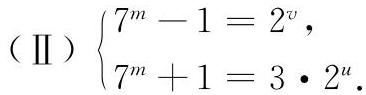
\includegraphics[max width=\textwidth, center]{2024_10_09_7e48ff928cc374c97394g-120}

对(II)中 $7^{m}+1=3 \cdot 2^{u}$ 两边模 3 可得矛盾. \\
对(I )中 $7^{m}+1=2^{v}$ 讨论,可知 $v \geqslant 3$ ,两边模 8 知 $m$ 为奇数. \\
若 $m=1$ ,则 $v=3$ ,进而由

得\\
故\\
\begin{align*}
\begin{gathered}
7^{m}-1=3 \cdot 2^{u} \\
u=1 \\
y=u+v=4
\end{gathered}
\end{align*}

若 $m>1$ ,则\\
\begin{align*}
7^{m}+1=8 \cdot\left(7^{m-1}-7^{m-2}+\cdots-7+1\right)
\end{align*}

其中 $7^{m-1}-7^{m-2}+\cdots-7+1$ 是奇数个奇数之和,与 $7^{m}+1=2^{u}$ 矛盾.\\
综上,满足条件的 $(x, y)=(1,1),(2,4)$ . \\
22. 有两种情形,即\\
\begin{align*}
3^{a}-2^{b}=41 \text {, 或 } 2^{b}-3^{a}=41 \text {. }
\end{align*}

对后者可知 $b>3$ ,两边模 8 ,要\\
\begin{align*}
3^{a} \equiv 7(\bmod 8)
\end{align*}

但对任意非负整数 $a$ ,有\\
\begin{align*}
3^{a} \equiv 1 \text { 或 } 3(\bmod 8),
\end{align*}

矛盾.\\
现在只需讨论 $3^{a}-2^{b}=41$ 的情形. \\
此时,对等式两边模 3 ,知\\
\begin{align*}
2^{b} \equiv 1(\bmod 3)
\end{align*}

故 $b$ 为偶数,又显然 $b \neq 0$ ,可设 $b=2 n, n$ 为正整数. \\
对等式两边模 4 ,得\\
\begin{align*}
3^{a} \equiv 1(\bmod 4)
\end{align*}

故 $a$ 为偶数,设 $a=2 m$ ,就有

故\\
\begin{align*}
\begin{gathered}
\left(3^{m}-2^{n}\right)\left(3^{m}+2^{n}\right)=41 \\
\left(3^{m}-2^{n}, 3^{m}+2^{n}\right)=(1,41)
\end{gathered}
\end{align*}

这导致 $2 \cdot 3^{m}=42$ ,即 $3^{m}=21$ ,矛盾. \\
所以,不存在符合要求的非负整数 $a ,  b$.\\
23. 注意到\\
\begin{align*}
36^{k}-5^{m} \equiv \pm 1(\bmod 6)
\end{align*}

故 $36^{k}-5^{m}$ 可能取到的正整数从小到大依次为 $1,11, \cdots$ . \\
现在若 $36^{k}-5^{m}=1$ ,则 $k>1$ ,故两边模 8 ,要求\\
\begin{align*}
5^{m} \equiv-1(\bmod 8)
\end{align*}

但 $5^{m} \equiv 1$ 或 $5(\bmod 8) ,$ 矛盾.\\
另外,当 $k=1, m=2$ 时, $36^{k}-5^{m}=11$ . 所以, $36^{k}-5^{m}$ 所能取到的最小正整数为 11 .

现在考虑 $5^{m}-36^{k}$ 所能取到的最小正整数,由\\
\begin{align}
& 5^{m}-36^{k} \equiv 4(\bmod 5) \\
& 5^{m}-36^{k} \equiv \pm 1(\bmod 6)
\end{align}

可知\\
\begin{align*}
5^{m}-36^{k} \geqslant 19
\end{align*}

综上可知, $\left|36^{k}-5^{m}\right|$ 的最小可能值为 11.\\
24. 对方程两边模 3 , 可知 $z$ 为偶数, 所以 $3^{x}+2^{2 y}$ 是一个完全平方数. 这样,利用 3.2 节例 11 的结论,可知 $x=y=z=2$ . \\
25. 由条件, 知 $x^{2}+y^{2}=z^{2}$ 且 $x+z=2 y$, 则\\
\begin{align*}
y^{2}=(z-x)(z+x)=2 y(z-x)
\end{align*}

即\\
\begin{align*}
y=2(z-x)
\end{align*}

于是 $y$ 为偶数,设 $y=2 m$ ,则

解得\\
\begin{align*}
\begin{gathered}
x+z=4 m, z-x=m \\
x=\frac{3 m}{2}, z=\frac{5 m}{2}
\end{gathered}
\end{align*}

故 $m$ 为偶数. 因此\\
\begin{align*}
(x, y, z)=(3 n, 4 n, 5 n)
\end{align*}

这里 $n=\frac{m}{2}$ 为正整数.\\
26. 因为 $A E \cdot B E=D E \cdot E G$ ,而 $E G=E F+F G=A E+D E$ (用到 $D G / /$ $B C)$ ,故\\
\begin{align*}
x(86-x)=y(x+y)
\end{align*}

对等式中的 $x ,  y$ 作奇偶分析,可知 $x ,  y$ 都为偶数. 

将它变形为 $\left(x+\frac{y}{2}-43\right)^{2}+y^{2}=\left(43-\frac{y}{2}\right)^{2}$,\\
故存在正整数 $a ,  b ,  k$, 使得\\
\begin{align*}
y=2 a b k, 43-\frac{y}{2}=\left(a^{2}+b^{2}\right) k
\end{align*}

所以\\
\begin{align*}
\left(a^{2}+a b+b^{2}\right) k=43,
\end{align*}

于是\\
\begin{align*}
k=1,(a, b)=(6,1),(1,6) .
\end{align*}

从而 $y=12$ (此时 $x=2$ 或者 72).\\
27. 只需考虑素数的幂的形式的数 $n$. 为此, 取素数 $p$, 使 $p \equiv 3(\bmod 4)$ (例如 $7,11,19 \cdots)$, 考虑数 $p^{2012}$ . 

利用 3.3 节例 2 中的方法, 可知数 $p^{2012}$ 不会是勾股三角形的斜边长.下证:不定方程 $x^{2}+p^{4024}=z^{2}$ 恰有 2012 组解. 事实上,因为\\
\begin{align*}
(z-x)(z+x)=p^{4024}
\end{align*}

故 $(z-x, z+x)=\left(1, p^{4024}\right),\left(p, p^{4023}\right), \cdots,\left(p^{2011}, p^{2013}\right)$,\\
结合 $p$ 为奇数, 可知求出的每一组 $(x, z)$ 都是正整数, 故 $p^{2012}$ 恰在 2012 组勾股数中出现. 

说明 此题的构造方法是基于因式分解,且由此方法可证:对任意正整数 $k$, 都有无穷多个正整数 $n$, 数 $n$ 恰好在 $k$ 组勾股数中出现.\\
28. 等价于求满足条件\\
\begin{align*}
x+y+z=x y
\end{align*}

的勾股数组 $(x, y, z)$.\\
注意到 $z=\sqrt{x^{2}+y^{2}}$, 于是(1)变为\\
\begin{align*}
x^{2}+y^{2}=(x y-x-y)^{2},
\end{align*}

即\\
\begin{align*}
x^{2}+y^{2}=x^{2} y^{2}-2 x y(x+y)+x^{2}+2 x y+y^{2},
\end{align*}

故\\
\begin{align*}
x^{2} y^{2}-2 x y(x+y)+2 x y=0,
\end{align*}

从而\\
\begin{align*}
x y-2(x+y)+2=0
\end{align*}

即\\
\begin{align*}
(x-2)(y-2)=2,
\end{align*}

得\\
\begin{align*}
(x, y)=(3,4),(4,3)
\end{align*}

综上, 所求直角三角形的三边长为 $3,4,5$.\\
29. 根据 3.3 节开始的分析, 注意到, 勾股三角形的面积还可以表示为\\
$k^{2} m n\left(n^{2}-m^{2}\right)$ 的形式,其中 $k ,  m ,  n$ 为正整数, $(m, n)=1, m<n, m$ 与 $n$一奇一偶. 于是 $k^{2} m n\left(n^{2}-m^{2}\right)=24=2^{3} \times 3$ ,故 $k=1$ 或 2 . 若 $k=1$ ,则由 $m ,  n$ 一奇一偶可知 $m ,  n$ 中有一个为 8 的倍数,这导致 $k^{2} m n\left(m^{2}-n^{2}\right) \geqslant 8 \times$ $3 \times\left(8^{2}-3^{3}\right)>24$ ,故 $k=2$ . 此时 $m n\left(n^{2}-m^{2}\right)=2 \times 3$ ,只能是 $(n, m)=$ $(2,1)$. 故满足条件的三角形只有一个,其边长为 $(6,8,10)$.\\
30. 设 $\triangle A B C$ 各顶点的对应边长为 $a ,  b ,  c$. 过 $A$ 作 $\angle A$ 的平分线交 $B C$于点 $D$, 则\\
\begin{align*}
C D=\frac{a b}{b+c}
\end{align*}

利用 $\triangle A C D \backsim \triangle B C A ,$ 可知\\
\begin{align*}
\frac{C D}{b}=\frac{b}{a}
\end{align*}

即\\
\begin{align*}
a^{2}=b(b+c)
\end{align*}

而\\
\begin{align*}
\angle C>90^{\circ}
\end{align*}

故\\
\begin{align*}
c^{2}>a^{2}+b^{2}
\end{align*}

由\\
\begin{align*}
a^{2}=b(b+c)
\end{align*}

设\\
\begin{align*}
(b, b+c)=d
\end{align*}

则 $(b, c)=d$ ,并且 $d^{2} \mid a^{2}$ ,故 $d \mid a$ . \\
为求 $a+b+c$ 的最小值, 可设 $d=1$, 这时, $b$ 与 $b+c$ 都为完全平方数,\\
设\\
\begin{align*}
b=m^{2}, b+c=n^{2}, m, n \in \mathbf{N}^{*}
\end{align*}

则 $a=m n$ . 利用 $a+b>c$ 及 $c^{2}>a^{2}+b^{2} ,$ 可知\\
\begin{align*}
m n+m^{2}>n^{2}-m^{2}
\end{align*}

且\\
\begin{align*}
\left(n^{2}-m^{2}\right)^{2}>(m n)^{2}+m^{4}
\end{align*}

于是\\
\begin{align*}
m>n-m
\end{align*}

即\\
\begin{align*}
n<2 m
\end{align*}

并且\\
\begin{align*}
n^{4}>3 m^{2} n^{2}
\end{align*}

即\\
\begin{align*}
n^{2}>3 m^{2}
\end{align*}

所以\\
\begin{align*}
3 m^{2}<n^{2}<4 m^{2}
\end{align*}

从而在 $3 m^{2}$ 与 $4 m^{2}$ 之间有一个完全平方数, 这要求 $m \geqslant 4$, 这时 $n \geqslant 7$,

故\\
\begin{align*}
a+b+c \geqslant 4 \times 7+7^{2}=77
\end{align*}

显然 $(a, b, c)=(28,16,33)$ 满足条件, 故所求 $\triangle A B C$ 周长的最小值为 77 . \\
31. 设整数 $a ,  b$ 满足 $5 a \geqslant 7 b \geqslant 0$. 令\\
\begin{align*}
w=\left[\frac{b}{5}\right]\left(\text { 表示不超过 } \frac{b}{5} \text { 的最大整数) }, v=b-5 w,\right.
\end{align*}

则当 $v=0,1,2,3,4$ 时( $v$ 只有这 5 种取值),将原方程组视为关于 $x ,  y ,  z$的不定方程组分别有非负整数解\\
\begin{align}
& (x, y, z) \\
= & (a-7 w, 0,0),(a-7 w-2,1,0),(a-7 w-3,0,1), \\
& (a-7 w-5,1,1),(a-7 w-6,0,2) .
\end{align}

所以,命题成立.\\
32. 当 $n>2 a b c-a b-b c-c a$ 时, 考虑不定方程\\
\begin{align*}
x b c+y c a+z a b=n
\end{align*}

的整数解 $(x, y, z)$.\\
\begin{align*}
\text { 令 } t=x b+y a, \text { 则 }(z, t) \text { 是方程 }
\end{align*}\\
\begin{align*}
c t+z a b=n
\end{align*}

的整数解,故可设 $0 \leqslant z<c$ (注意,这里用到 $(c, a b)=1$ 时 (2) 有解),这时由 (2)知\\
\begin{align}
t & =\frac{n-z a b}{c} \\
& \geqslant \frac{n-a b(c-1)}{c} \\
& >\frac{a b c-b c-c a}{c} \\
& =a b-b-a
\end{align}

而由 3.1 节例 3 的结论,知 $x b+y a=t$ 有非负整数解. 所以,此时(1)有非负整数解.

下证:当 $n=2 a b c-a b-b c-c a$ 时,(1)没有非负整数解.\\
事实上,若存在非负整数组 $(x, y, z)$ 满足\\
\begin{align*}
x b c+y c a+z a b=2 a b c-a b-b c-c a
\end{align*}

则\\
\begin{align*}
(x+1) b c+(y+1) c a+(z+1) a b=2 a b c
\end{align*}

利用 $a ,  b ,  c$ 两两互素, 可知

导致\\
\begin{align*}
a|x+1, b| y+1, c \mid z+1
\end{align*}\\
\begin{align}
2 a b c & =(x+1) b c+(y+1) c a+(z+1) a b \\
& \geqslant a b c+b c a+c a b=3 a b c
\end{align}

矛盾. 所以命题成立.\\
33. 设 $n$ 是一个满足条件的数, 则 $n>1$, 且此时只有一个数 (即 1 ) 既是 $n$的因数, 又是与 $n$ 互素的数. 故 $1,2, \cdots, n$ 中恰好有一个数, 它既不是 $n$ 的因数, 又不与 $n$ 互素.

由于 $n>1$ 时, $\varphi(n)$ 为偶数, 若 $n$ 为偶数, 则在 $n \geqslant 10$ 时, 数 $n-2$ 与 $n-4$既不与 $n$ 互素, 又不是 $n$ 的因数, 故 $n \geqslant 10$ 且 $n$ 为偶数时, $n$ 不满足条件; 若 $n$为奇数, 则 $d(n)$ 为奇数, 此时 $n$ 是一个完全平方数. 设 $n=(2 m+1)^{2}$, 若 $m>1$, 则数 $n-(2 m+1)$ 和 $n-2(2 m+1)$ 都不是 $n$ 的因数, 且都不与 $n$ 互素, 此时, $n$ 不满足条件. 

综上, 只需对 $n=2,4,6,8,9$ 进行验算, 可知满足条件的 $n=6,8,9$.\\
34. 我们利用勾股数来构造. 任取一组勾股数 $(x, y, z)$ (不必是本原的),令\\
\begin{align*}
a=x\left|4 y^{2}-z^{2}\right|, b=y\left|4 x^{2}-z^{2}\right|, c=4 x y z
\end{align*}

则有\\
\begin{align}
a^{2}+b^{2} & =x^{2}\left(3 y^{2}-x^{2}\right)^{2}+y^{2}\left(3 x^{2}-y^{2}\right)^{2} \\
& =x^{6}+3 x^{2} y^{4}+3 x^{4} y^{2}+y^{6} \\
& =\left(x^{2}+y^{2}\right)^{3}=\left(z^{3}\right)^{2} \\
& a^{2}+c^{2}=x^{2}\left(4 y^{2}+z^{2}\right)^{2} \\
& b^{2}+c^{2}=y^{2}\left(4 x^{2}+z^{2}\right)^{2}
\end{align}

由于勾股数有无穷多组, 从而符合条件的三元正整数数组有无穷多组.\\
例如: 当 $x=3, y=4, z=5$ 时, 得出\\
\begin{align*}
a=117, b=44, c=240
\end{align*}

并且\\
\begin{align*}
117^{2}+44^{2}=125^{2}, 117^{2}+240^{2}=267^{2}, 44^{2}+240^{2}=244^{2}
\end{align*}\\
35. 两边模 11, 由 Fermat 小定理知, 当 $11 \nmid y$ 时, 有\\
\begin{align*}
y^{10} \equiv 1(\bmod 11)
\end{align*}

故此时\\
所以总有\\
即\\
另一方面,对 $x^{2}$ 而言,由于\\
\begin{align*}
x \equiv 0, \pm 1, \pm 2, \pm 3, \pm 4, \pm 5(\bmod 11)
\end{align*}

故\\
\begin{align*}
x^{2} \equiv 0,1,4,9,5,3(\bmod 11)
\end{align*}

所以, $x^{2}=y^{5}-4$ 没有整数解. \\
36. 两边模 13 去处理. 由 Fermat 小定理知, 当 $13 \nmid m$ 时,有 $m^{12} \equiv 1(\bmod 13)$ ,得 $m^{6} \equiv 1$ 或 $25(\bmod 13)$ ,所以, $m^{3} \equiv \pm 1$ 或 $\pm 5(\bmod 13)$ ,即总有 $m^{3} \equiv 0,1$ , $5,8,12(\bmod 13)$.

与上题类似,可知 $n^{2} \equiv 0,1,4,9,3,12(\bmod 13)$ ,于是, $n^{4} \equiv 0,1,3$ 或 $9(\bmod 13)$ . 

利用上述结论,可知,对正整数 $m ,  n$ ,总有\\
\begin{align*}
m^{3}+n^{4} \equiv 0,1,2,3,4,5,6,8,9,10,11,12(\bmod 13)
\end{align*}

即 $m^{3}+n^{4} \not \equiv 7(\bmod 13)$.\\
然而, $19^{19} \equiv 6^{19} \equiv 6^{7} \equiv-6 \equiv 7(\bmod 13)$ (这里用到 Fermat 小定理及 $\left.6^{6} \equiv-1(\bmod 13)\right)$.

所以,不存在使 $19^{19}=m^{3}+n^{4}$ 成立的正整数 $m ,  n$ . \\
说明 上述两题中模参数的选择是基于 Fermat 小定理的反用(第 35 题中, 2,5 都是 $11-1$ 的因数,而第 36 题中, 3,4 都是 $13-1$ 的因数),此时所涉幂次对模参数所得的余数相对容易控制,从而能一步到位导出矛盾. \\
37. 注意到 $(x, y, z, u, v)=(1,2,3,4,5)$ 是原方程的正整数解.

一般地,设 $(x, y, z, u, v)$ 是原方程的正整数解,且 $x<y<z<u<v ,$则将原方程视为关于 $x$ 的一元二次方程,利用韦达定理可知( $y z u v-x, y$ , $z, u, v)$ 也是原方程的正整数解,依对称性,可知 $(y, z, u, v, y z u v-x)$ 也是解,并且满足条件 $y<z<u<v<y z u v-x$ . 依此递推方式,可得原方程的无穷多组正整数解,并且后一步构造的解中,最小的数比前一组解中最小的数大.

所以,存在满足条件的正整数解. \\
38. 分别就 $a$ 的不同情况讨论方程\\
\begin{align*}
x^{2}+a x y+y^{2}=1
\end{align*}

的整数解的组数.\\
当 $a=0$ 时, 方程为 $x^{2}+y^{2}=1$, 仅有 4 组整数解.\\
若 $a \neq 0$, 则 $(x, y)$ 为方程 (1) 的解的充要条件是: $(x,-y)$ 为方程 $x^{2}-$ $a x y+y^{2}=1$ 的解. 所以, 只需讨论 $a<0$ 且方程 (1) 有无穷多组非负整数解 $(x, y)$ 的情形.

若 $a=-1$, 则 (1) 为 $x^{2}-x y+y^{2}=1$, 两边乘以 4 , 再配方得 $(2 x-y)^{2}+$ $3 y^{2}=4$ ,仅有两组非负整数解. 

如果 $a<-1$, 那么 $(-a, 1)$ 为(1)的一组正整数解. 一般地, 设 $(x, y)$ 为(1)的正整数解, 且 $x>y$, 则 $(x,-a x+y)$ 也是(1)的解 (这一个解, 在视(1)为关于 $y$ 的一元二次方程时, 利用韦达定理可得), 当然 ( $-a x+y, x$ )(满足 $-a x+y>x>y)$ 也是(1)的正整数解, 依此递推, 可知这时(1)有无穷多组正整数解.

综上所述,当 $|a|>1$ 时, 方程(1)有无穷多组整数解,而 $|a| \leqslant 1$ 时, (1)仅有有限组整数解.\\
39. 由条件可知 $x \geqslant 2$.

如果 $n$ 为偶数, 那么由完全平方数 $\equiv 0$ 或 $1(\bmod 3)$ 可知 $x^{n} \equiv 0$ 或 $1(\bmod 3)$ ,但 $3^{k}-1 \equiv 2(\bmod 3)$ ,此时无解. 

如果 $n$ 为奇数, 那么\\
\begin{align*}
3^{k}=x^{n}-1=(x+1)\left(x^{n-1}-x^{n-2}+\cdots-x+1\right) .
\end{align*}

所以, $x+1$ 和 $A=x^{n-1}-x^{n-2}+\cdots-x+1$ 都为 3 的幂次. \\
注意到,\\
\begin{align*}
A \equiv(-1)^{n-1}-(-1)^{n-2}+\cdots-(-1)+1=n(\bmod (x+1))
\end{align*}

故 $n$ 为 3 的倍数. 可设 $n=3 m$, 记 $y=x^{m}$, 则\\
\begin{align*}
3^{k}=y^{3}+1=(y+1)\left(y^{2}-y+1\right)
\end{align*}

从而, $y+1$ 和 $y^{2}-y+1$ 都是 3 的幂次.\\
设 $y+1=3^{t}$ ,则由(1)知\\
\begin{align*}
3^{k}=\left(3^{t}-1\right)^{3}+1=3^{3 t}-3^{2 t+1}+3^{t+1} .
\end{align*}

如果 $t>1$, 那么 $3 t>2 t+1>t+1$, 此时 $3^{t+1} \| 3^{3 t}-3^{2 t+1}+3^{t+1}$, 对比 (2) 式两边要求 $k=t+1$, 但此时 (2) 的左边小于右边. 所以, $t=1$, 进而, $y=2, k=2$.得 $(x, k, n)=(2,2,3)$.

综上可知, 符合条件的正整数 $(x, k, n)=(2,2,3)$.\\
40. 记 $F(x, y)=x^{3}-x^{2} y+y^{2}+x-y$, 则 $F(1,1)=1, F(1,2)=2$.

因此, $n=1,2$ 时, 方程有正整数解.\\
下证: $F(x, y)=3$ 没有正整数解. \\
视方程 $F(x, y)=3$ 为关于 $y$ 的一元二次方程\\
\begin{align*}
y^{2}-\left(x^{2}+1\right) y+x^{3}+x-3=0
\end{align*}

如果存在正整数解, 那么\\
\begin{align*}
\Delta=\left(x^{2}+1\right)^{2}-4\left(x^{3}+x-3\right)=x^{4}-4 x^{3}+2 x^{2}-4 x+13
\end{align*}

\section{是一个完全平方数.}
注意到,当 $x \geqslant 2$ 时,有 $\Delta<\left(x^{2}-2 x-1\right)^{2}$ ,而 $x \geqslant 6$ 时,有 $\Delta>\left(x^{2}-\right.$ $2 x-2)^{2}$, 故 $x \geqslant 6$ 时, $\Delta$ 不是完全平方数. 而当 $x=1,2,3,4,5$ 时, 对应的 $\Delta=8,-3,-8,29,168$ 都不是完全平方数,故 $n=3$ 时无正整数解. 

综上可知, 所求的最小正整数 $n=3$.



\end{comment}